\chapter{Computing Disparity Intervals and Propagate them to the DSM}\label{chap:epistemic_uncertainty}
\todoroman{Citer la publication d'origine pour les figure (license IEEE ``Copyright 2024 IEEE. Published in the 2024 IEEE International Geoscience and Remote Sensing Symposium (IGARSS 2024), scheduled for 7 - 12 July, 2024 in Athens, Greece. Personal use of this material is permitted. However, permission to reprint/republish this material for advertising or promotional purposes or for creating new collective works for resale or redistribution to servers or lists, or to reuse any copyrighted component of this work in other works, must be obtained from the IEEE. Contact: Manager, Copyrights and Permissions / IEEE Service Center / 445 Hoes Lane / P.O. Box 1331 / Piscataway, NJ 08855-1331, USA. Telephone: + Intl. 908-562-3966.'')}

The previous chapter detailed the propagation of  uncertainty in a stereo matching problem, using the $\SAD$ function to compute the cost volume. However, real cases of stereo matching usually do not use such simple cost functions, but rather more complex ones. In particular, the CARS pipeline that will process the \acrshort{co3d} data will use the CENSUS and MC-CNN cost functions  \cite{zabih_non-parametric_1994,zbontar_stereo_2016} to compute the cost volume, followed by a \acrshort{sgm} regularization. Those methods produce far better results and are thus favored for stereo pipelines. Unfortunately, we are not able to propagate the uncertainty to those cost functions and regularization as we did in the previous chapter as it would be too complex and computationally heavy. The same observation can be made for any deep leaning method \cite{laga_survey_2022} as the data is processed through many consecutive layers. Furthermore, the previous chapter was restricted to the propagation of the uncertainty from input images to the cost volume, but did not attempt to quantify the uncertainty of the stereo matching process itself, \ie the algorithm ability to correctly\commanue{properly? c'est pour éviter la répétition avec correct, à moins que ce soit voulu} identify the correct disparity. A bad performing stereo matching algorithm can produce errors of great magnitude regardless of the uncertainty on input images, while more advanced algorithm may even present good performance despite noised input images. Using the semantics of this thesis, we will refer to the uncertainty of the stereo algorithm itself as its epistemic uncertainty. Indeed, it does not result form any aleatoric process, but rather a lack of knowledge on how to correctly and automatically identify the correct disparity\commanue{pareil tu as une répétition entre correctly et correct dans la phrase}.

This aforementioned epistemic uncertainty\commanue{alors moi perso je mettrais This aforementioned epistemic uncertainty modeling in stereo matching mais c'est pas une obligation} has been the subject of many works in the literature \cite{hu_quantitative_2012,  poggi_confidence_2021,wang_uncertainty_2022}, designed for so-called ``classical methods'' using cost volumes obtained from cost functions, or for learning-based methods. This uncertainty is quantified using ``confidence measures'', associating a value between $0$ and $1$ to each predicted disparity, $0$ meaning that the prediction should be questioned,  and $1$ meaning that the prediction is most certainly correct. We refer to \Cref{sec:uncertainty_pandora} for more details on confidence measures in stereo matching pipelines. In this chapter, we will study how possibility distributions are able to model the epistemic uncertainty associated with a cost volume, and then deduce disparity confidence intervals from the possibility distribution. This approach is complementary to classical confidence estimations as it is not meant to indicate whether or not we trust a prediction but rather to provide information on \textit{where} the correct disparity should be. We then propagate those disparity confidence intervals in the rest of the stereo pipeline to obtain height confidence intervals, and evaluate their performances. Following discussions with users and experts working at CNES, IGN and more generally in the AI4GEO consortium, we decided to fix ourselves an objective of $90\%$ of correct confidence intervals.

\todoroman{Vérifier que dans le chapitre 1 j'insiste bien sur ce que c'est une cost curve}
\section{Producing Confidence Intervals}
This section will detail the method developed to create disparity confidence intervals in the stereo matching step of the pipeline. We will use possibility distributions to model the uncertainty associated with the available information and deduce confidence intervals from it.

It is important to keep in mind that we want intervals as precise as possible, while staying relatively small. Indeed, it would be easy to reach a $100\%$ precision by simply extending the intervals to the whole range of considered disparities. However, the intervals would not contain any relevant information. We therefore must maintain a trade-off between the precision of the intervals and their size. As stated previously, we fixed ourselves a $90\%$ precision objective. As for the criteria of maintaining small intervals, we will introduce in \Cref{sec:metrics_disparity} different metrics to quantify their size for further evaluation. Different parameters will be introduced in our method, and we chose their values accordingly with the precision/size trade-off mentioned above. We will also study different configuration of those parameters in annex. \todoroman{Mettre les analyses en annexe}

\subsection{Possibility Distributions as Uncertain Models for Cost Curves}
In this section, we will detail how possibility distributions can be used to model the epistemic uncertainty associated with cost curves. We first present a quick reminder of concepts and notations regarding cost volumes presented in \Cref{sec:stereo_matching}, as we will base our model on them. Cost volume based approaches, considered here, compare every pixel from the left image $I_L$ to pixels from the same row in the right image $I_R$, in a given disparity range. The comparison is done using a cost function $f$, measuring the dissimilarity between two windows centered around pixel $p$ and $q$. All evaluations using this cost function are stored in a cost volume $C_V$:
\begin{align}
	C_V(\rowcol, ~d) = f(I_L(\rowcol), I_R(\rowcol+d))
\end{align}
where $d$ is the considered disparity. In this chapter, we consider that the cost volume then\commanue{je mettrais pas le then} undergoes a \acrshort{sgm} regularization step, which modifies the cost values\commanue{its values} to take into account more global information. Based on the observation that the disparity map is usually piece-wise regular in a scene, \acrshort{sgm} regularization has been designed to increase the cost of disparities for which no consensus exist among neighboring pixels. This way, only disparities that seem plausible and relatively regular compared to neighboring disparities are favored in the cost volume.

For every pixel $(\rowcol)$ from the left image, we refer to its cost curve as the cost volume at coordinates $(row,~col)$ for every considered disparity $d$, \ie the cost volume for which we fixed the first two variables. Cost curves are of much importance as we estimate the disparity of a pixel solely based on its cost curve. Indeed, we define the predicted disparity $\tilde{d}$ of a pixel $(\rowcol)$ as:
\begin{align}
	\tilde{d} = \argmin_d C_V(\rowcol, ~d)
\end{align} 
\Cref{fig:tuto_dense_matching} presents a cost curve and its true disparity. We can see that the true disparity can be correctly estimated by looking at the minimum of the cost curve.
 
\begin{figure}
    \centering
    \begin{subfigure}[t]{0.073\linewidth}
        \centering
        
\includegraphics[width=\linewidth]{Images/Chap_5/tuto_left_patch.png}
        \caption{}
        \label{fig:tuto_a}
    \end{subfigure}
    \hfill\begin{subfigure}[t]{\linewidth}
        \flushright
        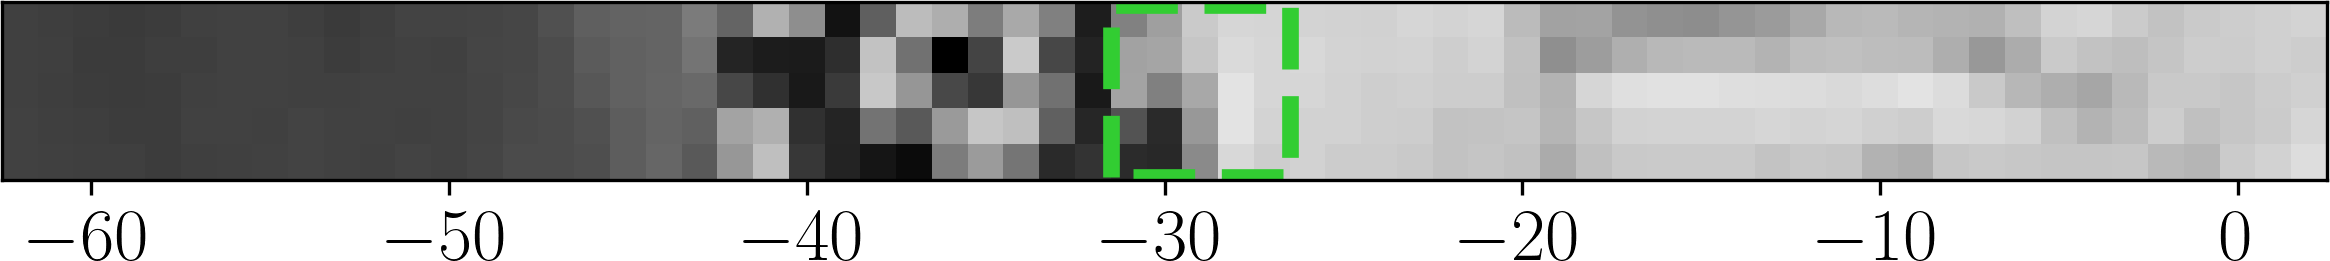
\includegraphics[width=0.927\linewidth]{Images/Chap_5/tuto_right_patch.png}
        \caption{}
        \label{fig:tuto_b}
    \end{subfigure}
    \begin{subfigure}[t]{\linewidth}
        \centering
        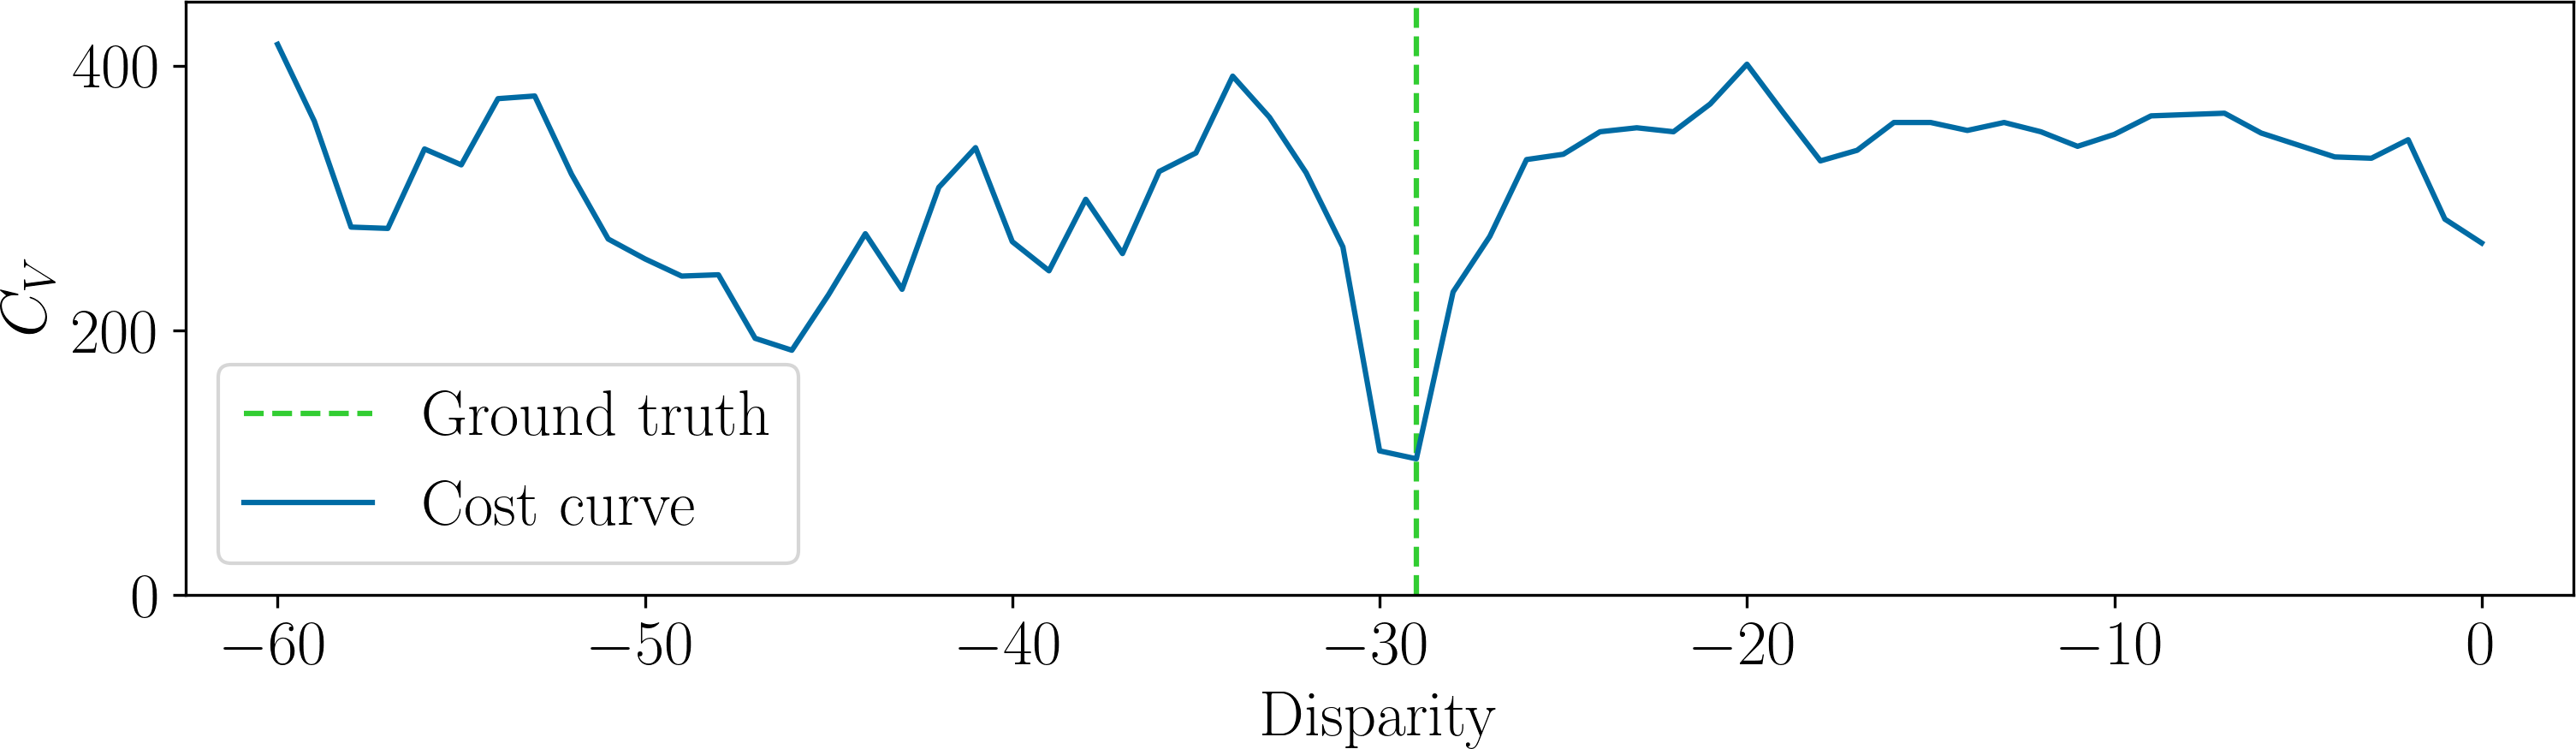
\includegraphics[width=\linewidth]{Images/Chap_5/tuto_cost_curve.png}
        \caption{Cost curve}
        \label{fig:tuto_c}
    \end{subfigure}
    \caption{Cost curve (\Cref{fig:tuto_c}) obtained from comparing a patch from the left image (\Cref{fig:tuto_a}) to patches from the right image (\Cref{fig:tuto_b}). The matching patch and its corresponding true disparity are indicated using dashed green lines.}
    \label{fig:tuto_dense_matching}
\end{figure}

In the following, we propose to consider possibility distributions to model the uncertainty associated with the choice of the predicted disparity from a cost curve. The values taken by possibility distributions will be based on the available information \ie the values of the cost volume. Before getting into details, let us justify this model. Possibility distributions are relatively simple model to use in comparison with imprecise probabilities or belief functions for instance, as we only need to specify a constraint on the atoms, and not on every event. As such, they have been used to model the uncertainty associated with an expert's opinion in applications such as groundwater contamination for instance in \cite{bardossy_l-_1995} and \cite{baudrit_joint_2007}. Since cost curves result in both:
\begin{itemize}
	\item dissimilarity measures between patches 
	\item a semi-global fusion of the information contained in the cost volume due to \acrshort{sgm} regularization
\end{itemize}it does not seem far-stretched to consider them equivalent to an expert stating his opinion on how likely two pixels should be matched. For this reason, possibility distributions seem appropriate to model the epistemic uncertainty of the cost volume.

In order to use possibility distributions, we first need to transform the available information, in our case the values contained in the cost curves, into degrees of possibility. \Cref{eq:possibility}\commanue{Plutôt que de faire référence à une équation située 100 pages avant, tu pourrais juste dire The definition of possibility distribution ou un truc équivalent} imposes that the values must lie between $0$ and $1$, and that the value $1$ must be attained at least once. We therefore propose to normalize each cost curve so that its minimal dissimilarity value equals a possibility degree of $1$, and that greater dissimilarity values are closer to $0$ in possibility. However, simply normalizing the values of each cost curve between $0$ and $1$ would artificially stretch the cost curve as seen in \Cref{fig:cost_curves_b}. It is especially blatant in the case for the orange dashed curve from \Cref{fig:cost_curves_a} as the range of its values is quite narrow compared to the blue curve, but they are both stretched to $[0,~1]$ in \Cref{fig:cost_curves_b}. In order to avoid this effect, we instead normalize every cost curve using the global minimum and global maximum of the cost volume, as:
\begin{align}
	C_V^{norm}(\rowcol, ~d) = \dfrac{C_V(\rowcol, ~d) - \max_{r,c,\delta}C_V(r,~c,~\delta)}{\min_{r,c,\delta}C_V(r,~c,~\delta) - \max_{r,c,\delta}C_V(r,~c,~\delta)}\label{eq:normalized_cost_curve}
\end{align}
Minima of the cost curve become maxima with this normalization. One problem remains, it is that unless the global maximum of the cost volume is attained in a cost curve, the normalized cost curve will never reach $1$. Therefore, it will not be a possibility distribution. This problem can be observed in \Cref{fig:cost_curves_c}. We thus add a constant to the normalized cost curve to obtain a possibility distribution $\pi_{row,~col}(d)$:
\begin{align}
	\pi_{row,~col}(d) = C_V^{norm}(\rowcol, ~d) + 1 - \max_\delta C_V^{norm}(\rowcol, ~\delta)\label{eq:possibility_cost_curve}
\end{align}
\Cref{fig:cost_curves_d} displays the possibility distributions obtained from the cost curves of \Cref{fig:cost_curves_a}.

\begin{figure}
    \centering
    \begin{subfigure}[t]{0.47\linewidth}
        \centering
        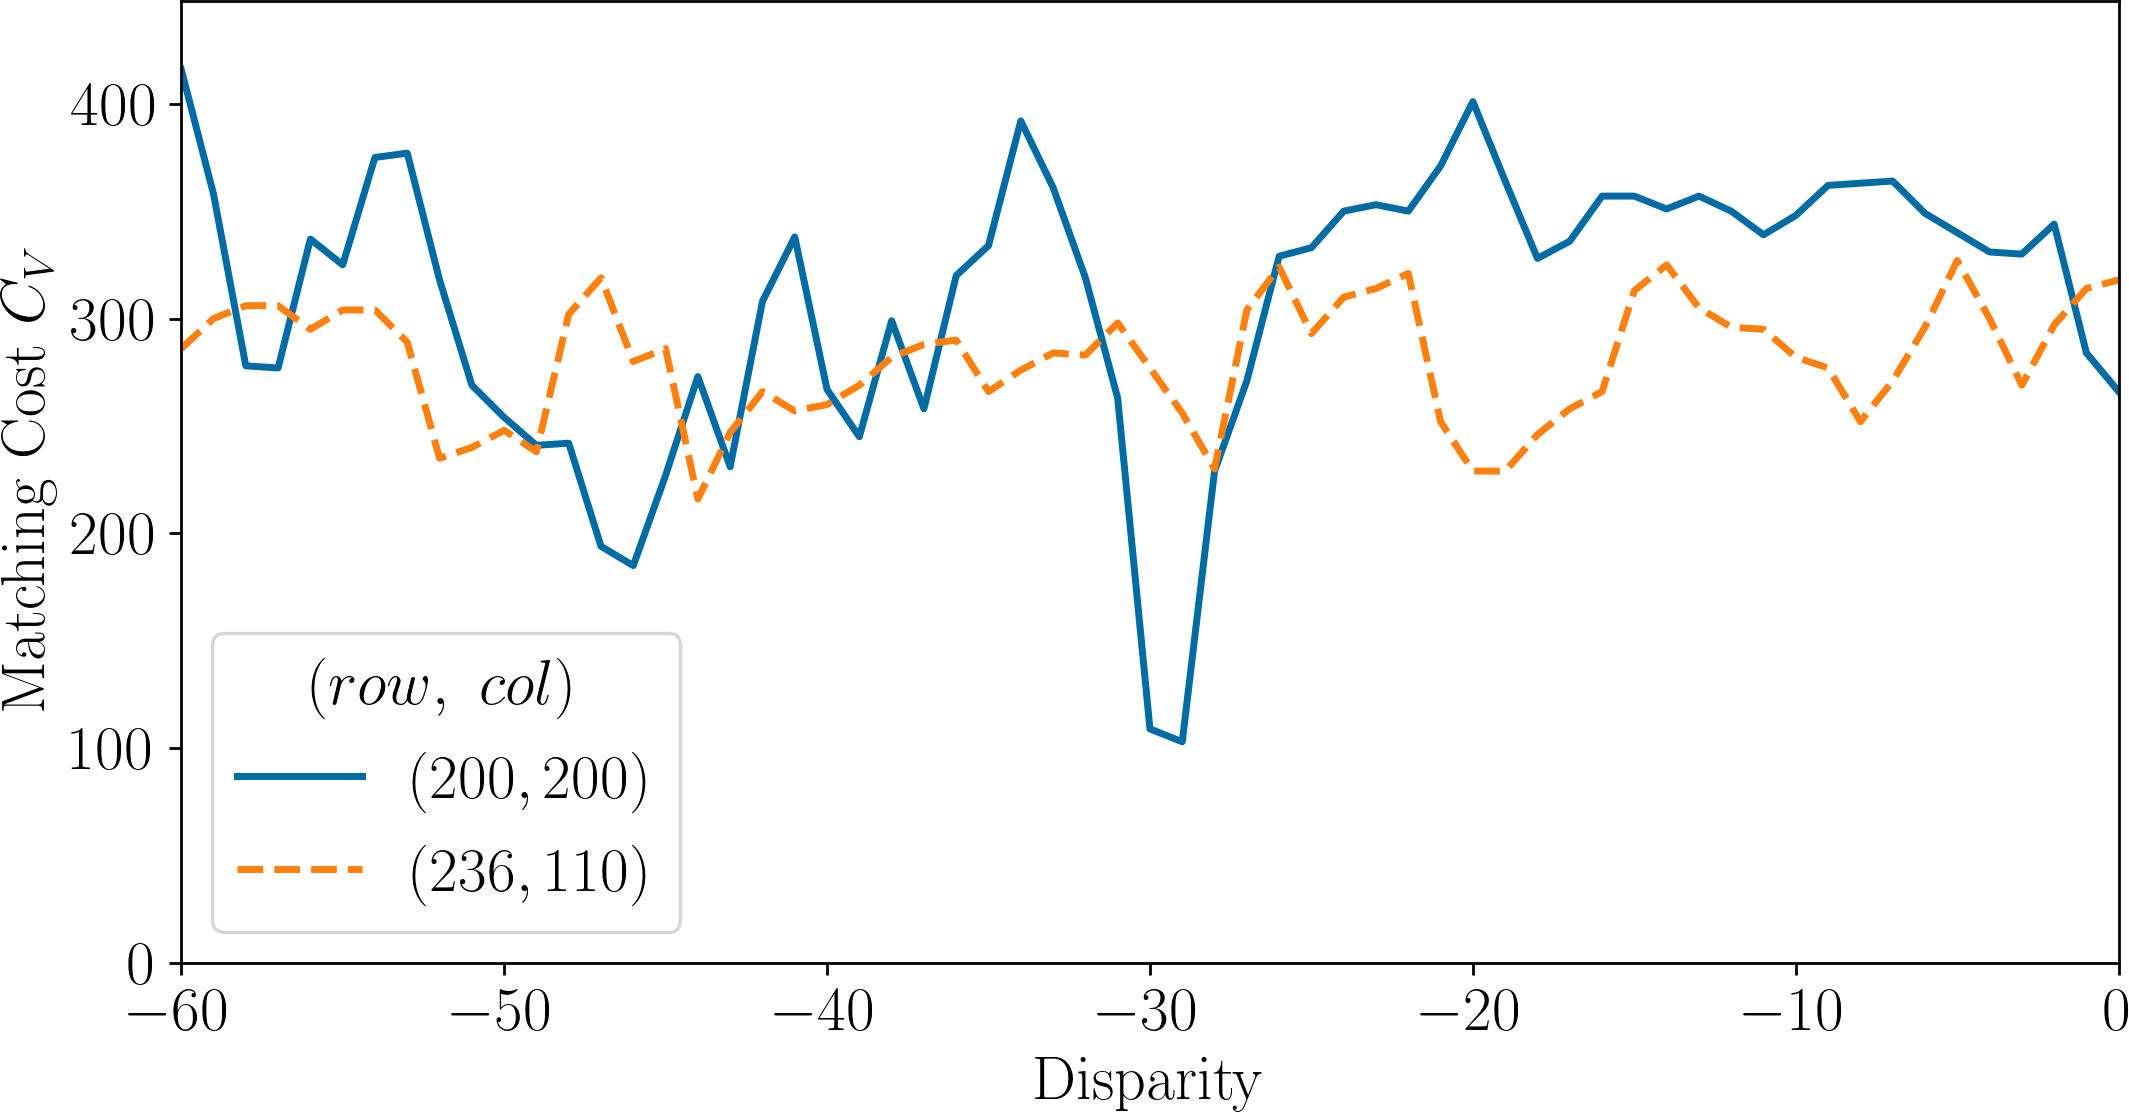
\includegraphics[width=\linewidth]{Images/Chap_5/cost_curve_not_normalized.png}
        \caption{Two cost curves}
        \label{fig:cost_curves_a}
    \end{subfigure}\hfill
    \begin{subfigure}[t]{0.47\linewidth}
        \centering
        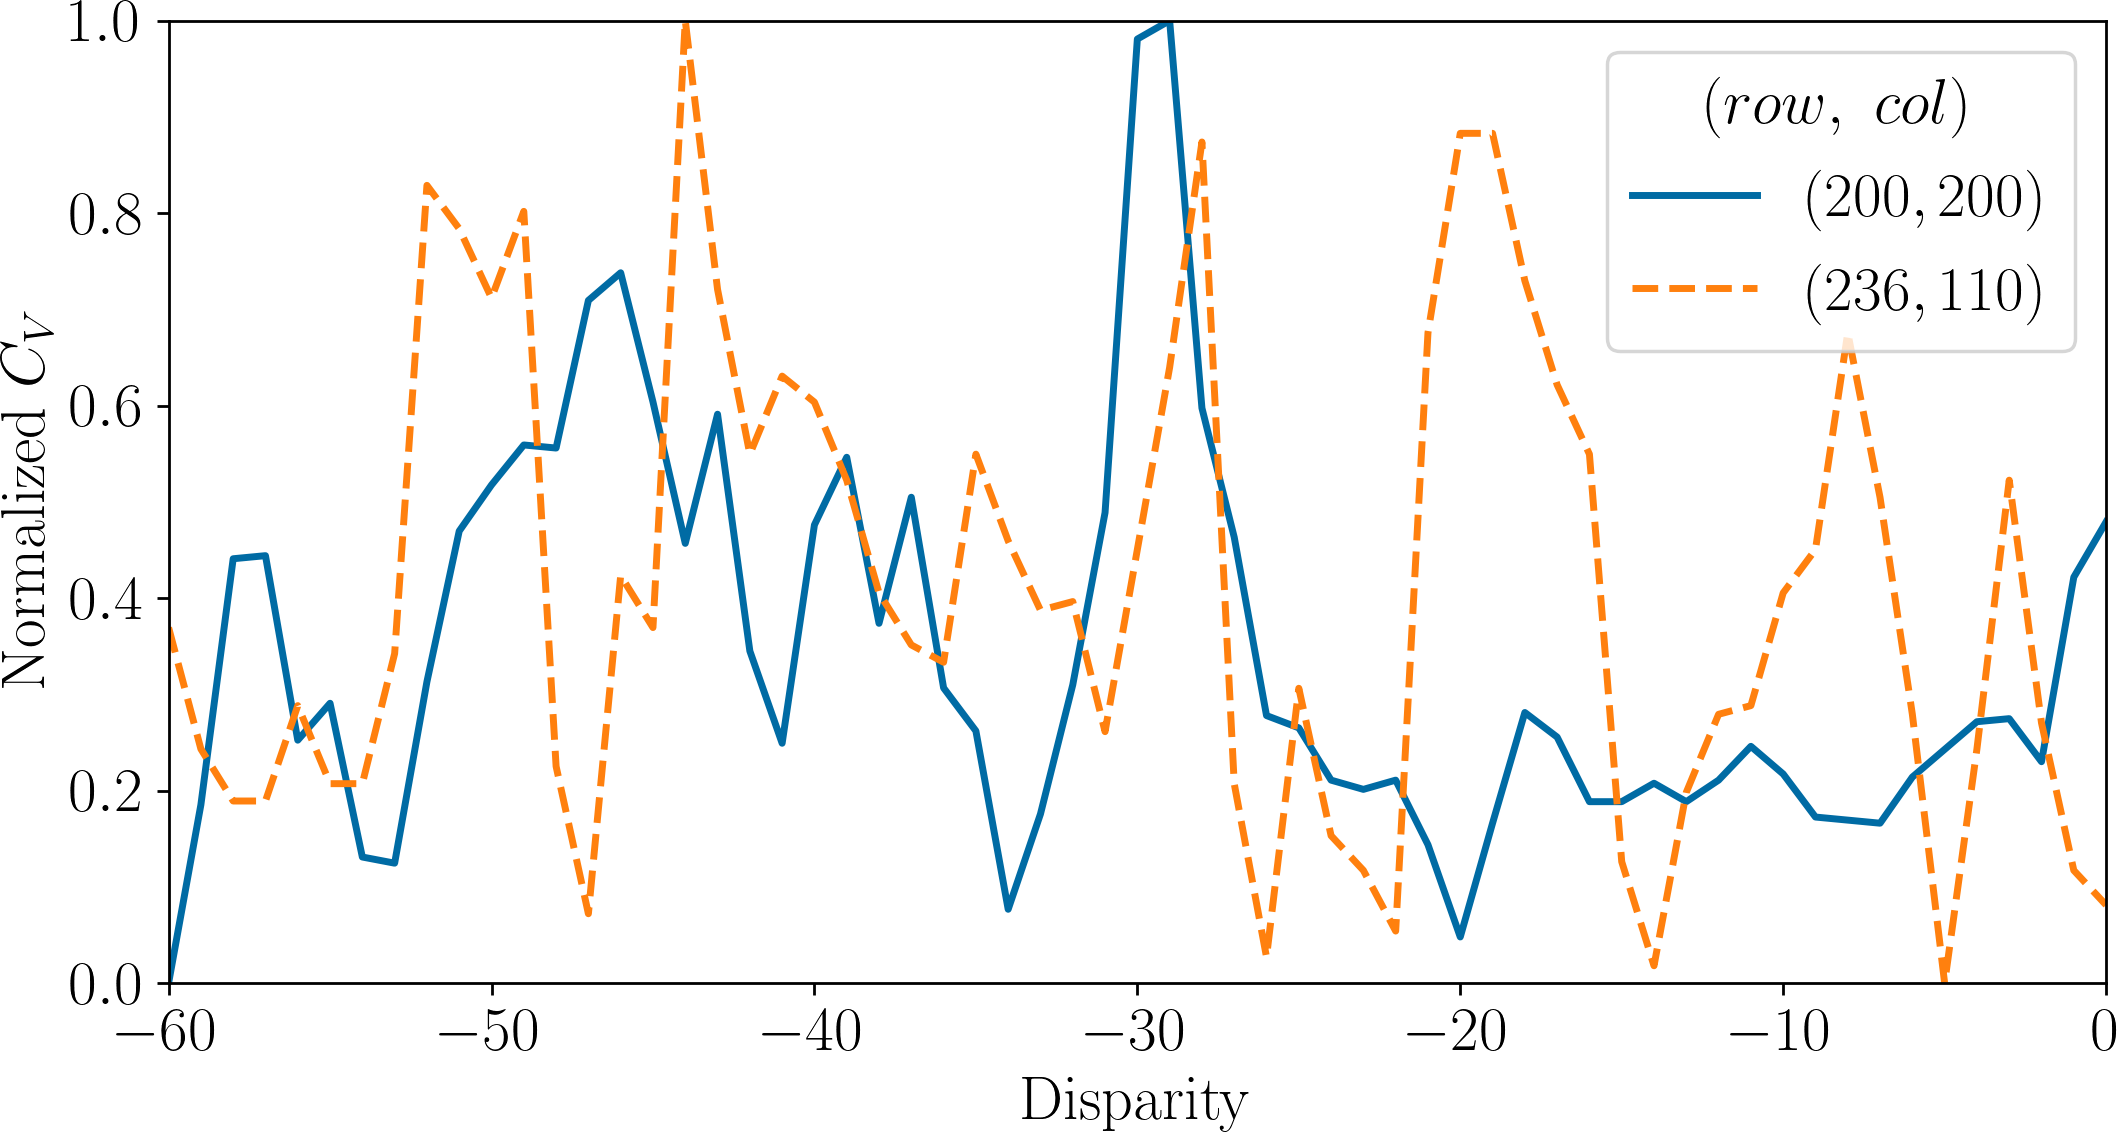
\includegraphics[width=\linewidth]{Images/Chap_5/cost_curve_bad_normalized.png}
        \caption{Normalized cost curves with local extrema}
        \label{fig:cost_curves_b}
    \end{subfigure}
    \begin{subfigure}[t]{0.47\linewidth}
        \centering
        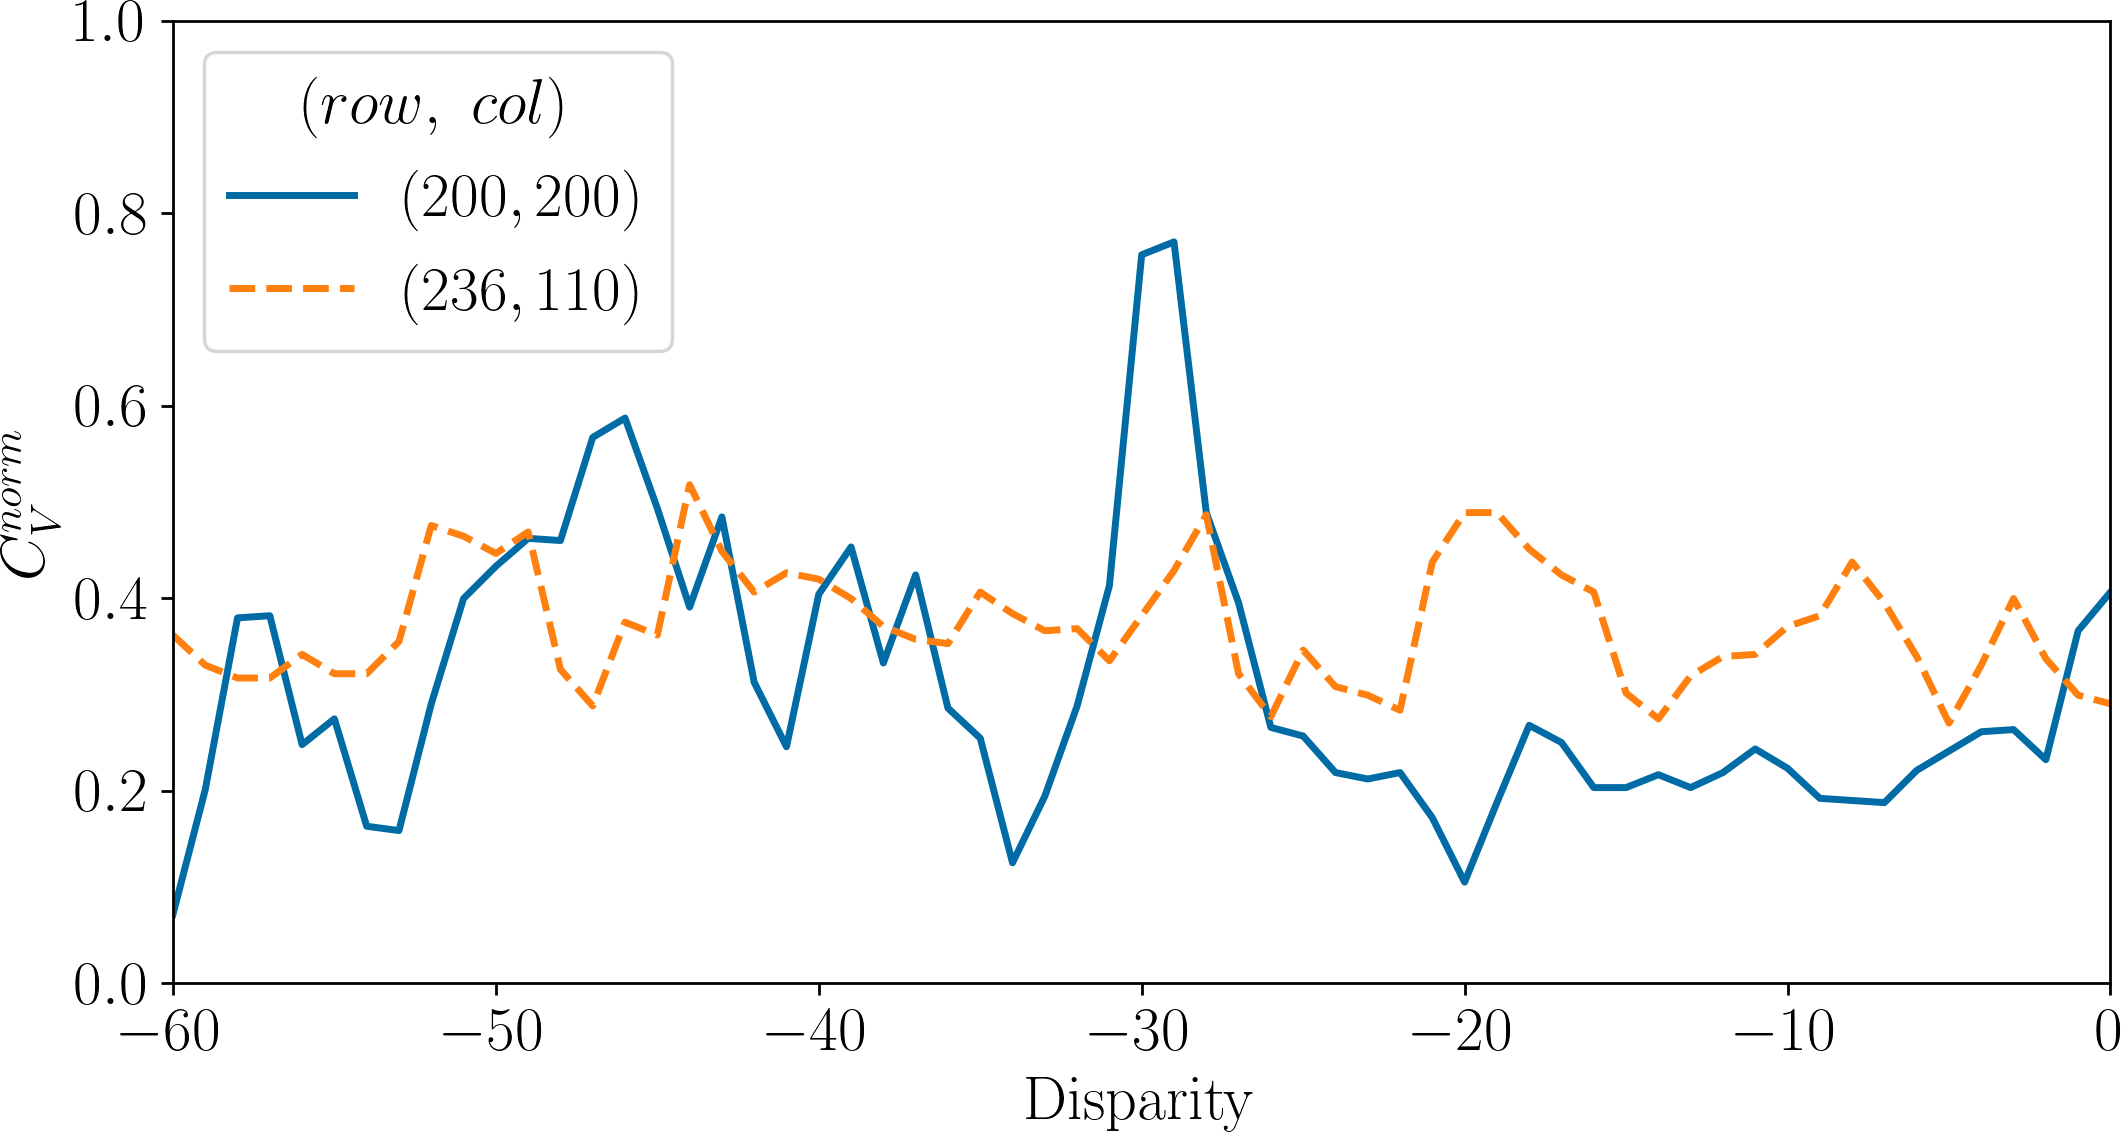
\includegraphics[width=\linewidth]{Images/Chap_5/cost_curve_normalized.png}
        \caption{Normalized cost curves $C_V^{norm}$ with global extrema}
        \label{fig:cost_curves_c}
    \end{subfigure}\hfill
    \begin{subfigure}[t]{0.47\linewidth}
        \centering
        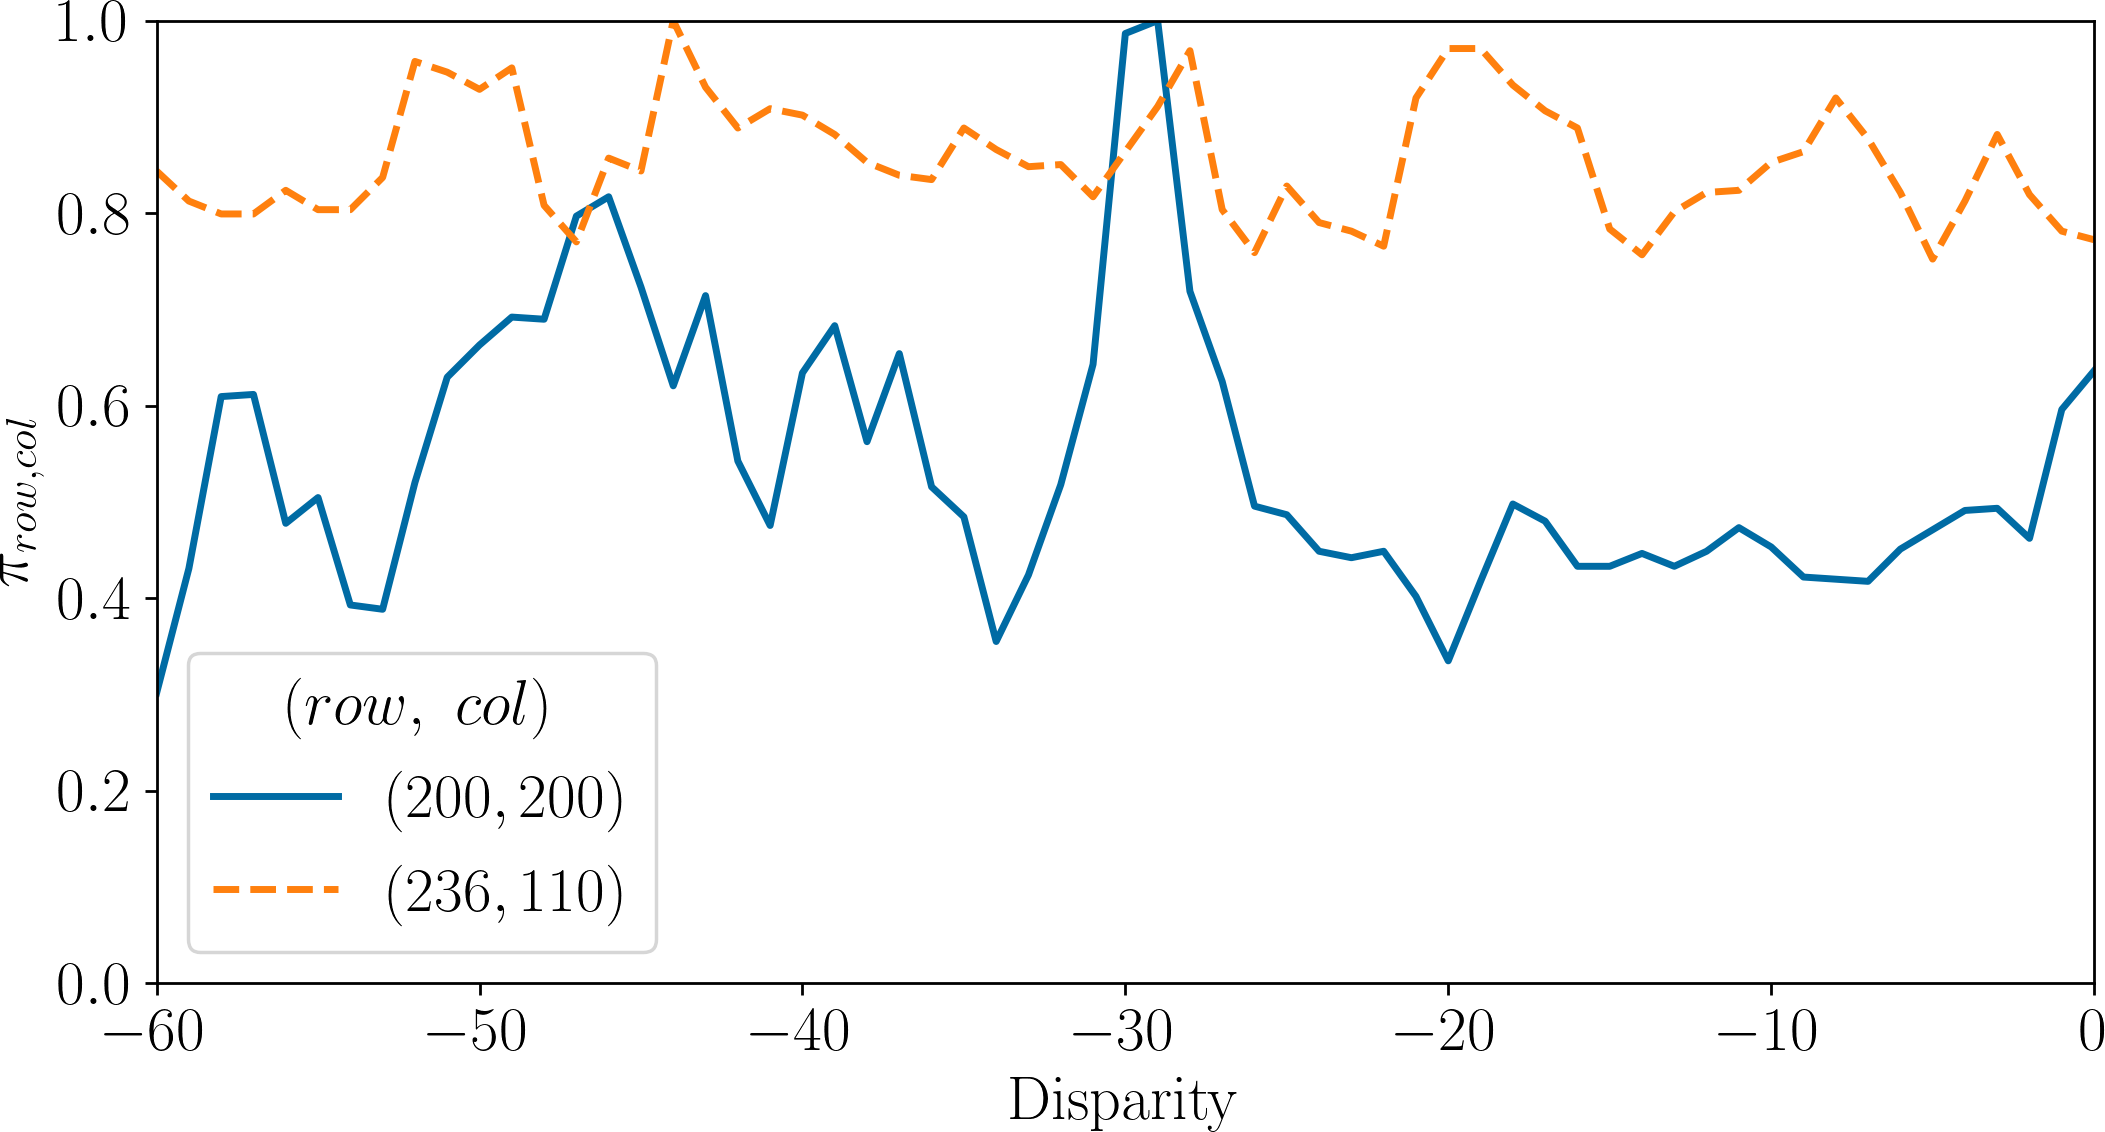
\includegraphics[width=\linewidth]{Images/Chap_5/cost_curve_possibility_distribution.png}
        \caption{Possibility distributions resulting from the cost curves}
        \label{fig:cost_curves_d}
    \end{subfigure}\hfill
    \caption{Transformation of cost curves (CENSUS + \acrshort{sgm} on Middlebury Cones) into possibility distributions. \Cref{fig:cost_curves_a} represents two cost curves that are normalized differently in \Cref{fig:cost_curves_b,fig:cost_curves_c}. \Cref{fig:cost_curves_d} uses the normalization of \Cref{fig:cost_curves_c} to create possibility distributions.}
    \label{fig:cost_curves_to_possibility}
\end{figure}

As stated previously, global extrema in \cref{eq:normalized_cost_curve} are employed to minimize the stretching effect when converting cost curves into possibility distributions. However, we also could have used the theoretical extrema of a cost curve instead. For instance, the CENSUS cost function on a $5\times5$ window provides values between $0$ and $C_{max}=24$. Adding \acrshort{sgm} regularization with penalty $P_2$ on $8$ directions yields cost volumes values between $0$ and $8\times(C_{max}+P_2)$ \cite{hirschmuller_accurate_2005}. However, this maximal cost is rarely attained in real case scenarios, and\commanue{je remplacerais and par therefore it} is too pessimistic and tends to over-compress the normalized cost curves. It is instead preferred to use global extrema of the cost volume for the normalization, as we suppose the best and worst match should have similar cost values across different scenes. This hypothesis is not restrictive for the images we consider in our stereo matching problem, as the size and diversity inside each scene lead to similar extrema. \todoroman{Faire relire la fin à Manue car le Balrog ne l'a pas lu} When processing very large images, CARS uses divide the image in smaller tiles that are process in parallel. We are not guaranteed that the cost volume extrema of each tile would be the same, but as they all come from the same image, it is not far-stretched to suppose differences in extrema are negligible. 

\subsection{From Possibilities to Disparity Confidence Intervals}
With the possibility distributions defined, our next objective is to establish a set of most possible disparities. We decided to aim for sets containing the true disparity $90\%$ of the time. This $90\%$ value was chosen following discussions with users and other experts working at CNES, IGN and more generally in the AI4GEO consortium. To define this set of most possible disparities, we compute the $\alpha$-cut (\cref{eq:alpha_cut}\commanue{tu fais un renvoi à l'équation, moi je renverrais à la définition. Bon c'est au même endroit de toute façon}) of the possibilities, or in other words, the set of all disparities $D_\alpha$ whose possibility is superior than $\alpha$:
\begin{align}
    D_\alpha=\{~ d ~|~ \pi_{\rowcol}(d)\geqslant\alpha\}\label{eq:set_of_possible_disparities}
\end{align}
By looking at possibility distributions obtained from different cost curves for which we know the true disparity, we first fixed the value $\alpha$ at $0.9$. In depth study of this parameter will be tested later, in order to see if it depends on the cost function, the type of scene considered, and to provide general guidelines on its optimal value. In the following, when the value of $\alpha$ is not specified, it will always be set at $0.9$. The fact that its value is the same as the $90\%$ confidence objective is a coincidence and one should not suppose that $\alpha$ and the confidence objective should be the same. Indeed raising the $\alpha$ value would decrease the size of the set $D_\alpha$ and therefore decrease the proportion of sets containing the true disparity, \ie the global confidence rate of intervals. \Cref{fig:disparity_intervals_a,fig:disparity_intervals_b} graphically represent $D_\alpha$ for the cost curves of \Cref{fig:cost_curves_to_possibility}.

\begin{remark}
    We are modelling the epistemic uncertainty of the cost curves using possibility distributions. In the rest of this chapter, we use a possibility distribution for each cost curve because we think it is a correct model in itself for the uncertainty we encounter. It is however possible to have a probabilistic interpretation of possibilities, which we will share in this remark as it may be of interest for people thinking the underlying uncertainty can be modeled by probabilities.
    
    We saw in \cref{eq:credal_set_possibility} from \Cref{chap:representation_of_uncertainty} that one way of interpreting $\pi_{\rowcol}$ is that it defines a set of probability distributions, \ie a credal set $\M$. We can also define $D_\alpha$ using this set $\M$, as:
    \begin{align}
        D_\alpha=\{~ d ~|~ \exists P\in\M ~\st~ P(d)\geqslant \alpha\}
    \end{align}
    or in plain words, $D_\alpha$ is the set of all disparities $d$ for which there exists a probability in $\M$ whose value is greater than $\alpha$ for $d$. We will not rely on this interpretation in the rest of this chapter, and instead only reason in terms of possibilities.
\end{remark}

\todoroman{Figure montrant différentes courbes de coût transformées, CENSUS MCCNN}

\Cref{eq:set_of_possible_disparities} defines a set of disparities $D_\alpha$ which is not necessarily convex. We will rather consider confidence disparity intervals $I_\alpha$ deduced from $D_\alpha$ in the rest of this chapter:
\begin{align}
    I_\alpha = [\underline{I}_\alpha,~\overline{I}_\alpha]=[\min D_\alpha, ~\max D_\alpha]\label{eq:confidence_disparity_intervals}
\end{align}
\Cref{fig:disparity_intervals_c,fig:disparity_intervals_d} graphically represent how $I_\alpha$ is determined for the two possibility distributions of the cost curves in \Cref{fig:cost_curves_to_possibility}. In the rest of this section, we will not make any distinction between disparity confidence intervals, disparity intervals, confidence intervals or simply intervals. A disparity interval is the convex envelope of its disparity set $D_\alpha$, which is a conservative approach as observed in \Cref{fig:disparity_intervals_b,fig:disparity_intervals_d}.

Considering intervals thus presents the advantage of working with convex sets and only requiring two scalars to describe the set. Users of the \acrshort{dsm}s produces by stereo photogrammetry are also used to consider confidence intervals \cite{oksanen_digital_2006, wang_robust_2015, panagiotakis_validation_2018, deschamps-berger_apport_2021, hugonnet_uncertainty_2022}. This will also facilitate further processing in the rest of the stereo pipeline, as we only need to take into account $2$ bounds to characterize the possible disparities, instead of a set of arbitrary shape. In the following figures, we use the same configuration for the correlator, \ie CENSUS cost function with \acrshort{sgm} regularization. We will study the influence of the cost function later\commanue{alors c'est bien de mentionner la conf utilisée. Après tant que tu utilises les figures juste à des fins explicatives c'est pas trop grave. Donc soit tu remontes cette info plus haut quand tu commences à faire des courbdes de coût. Soit tu gardes cette info quand tu en auras vraiment besoin pour valider ton approche. Histoire d'être sûr qu'entre temps les relecteurs n'aient pas oublié l'info. Là ça tombe un peu comme un cheveu sur la soupe dans ce paragraphe.}.

\begin{figure}
    \centering
    \begin{subfigure}[t]{0.47\linewidth}
        \centering
        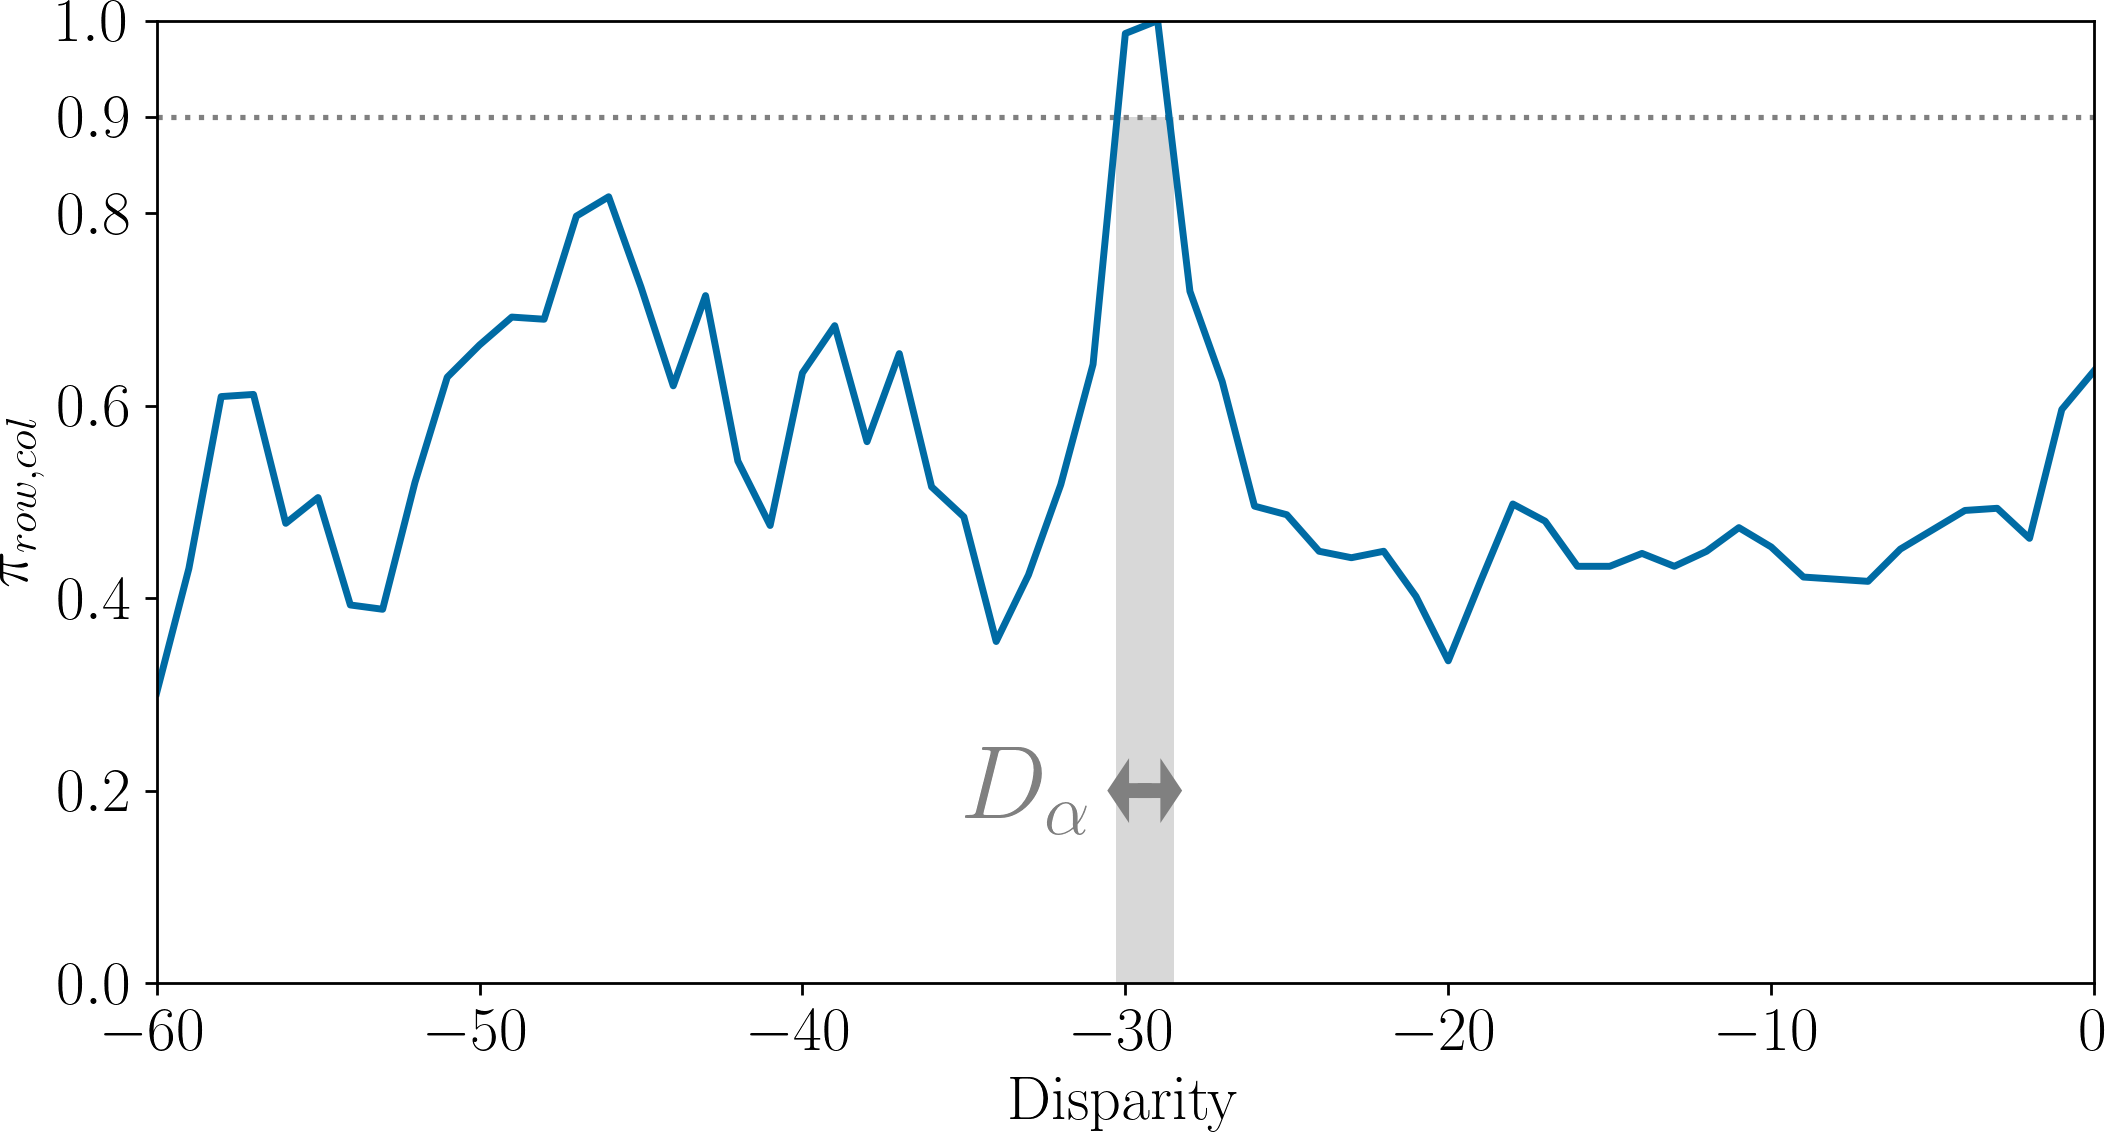
\includegraphics[width=\linewidth]{Images/Chap_5/disparity_interval_1.png}
        \caption{$D_\alpha$ for the blue possibility of \Cref{fig:cost_curves_d}}
        \label{fig:disparity_intervals_a}
    \end{subfigure}\hfill
    \begin{subfigure}[t]{0.47\linewidth}
        \centering
        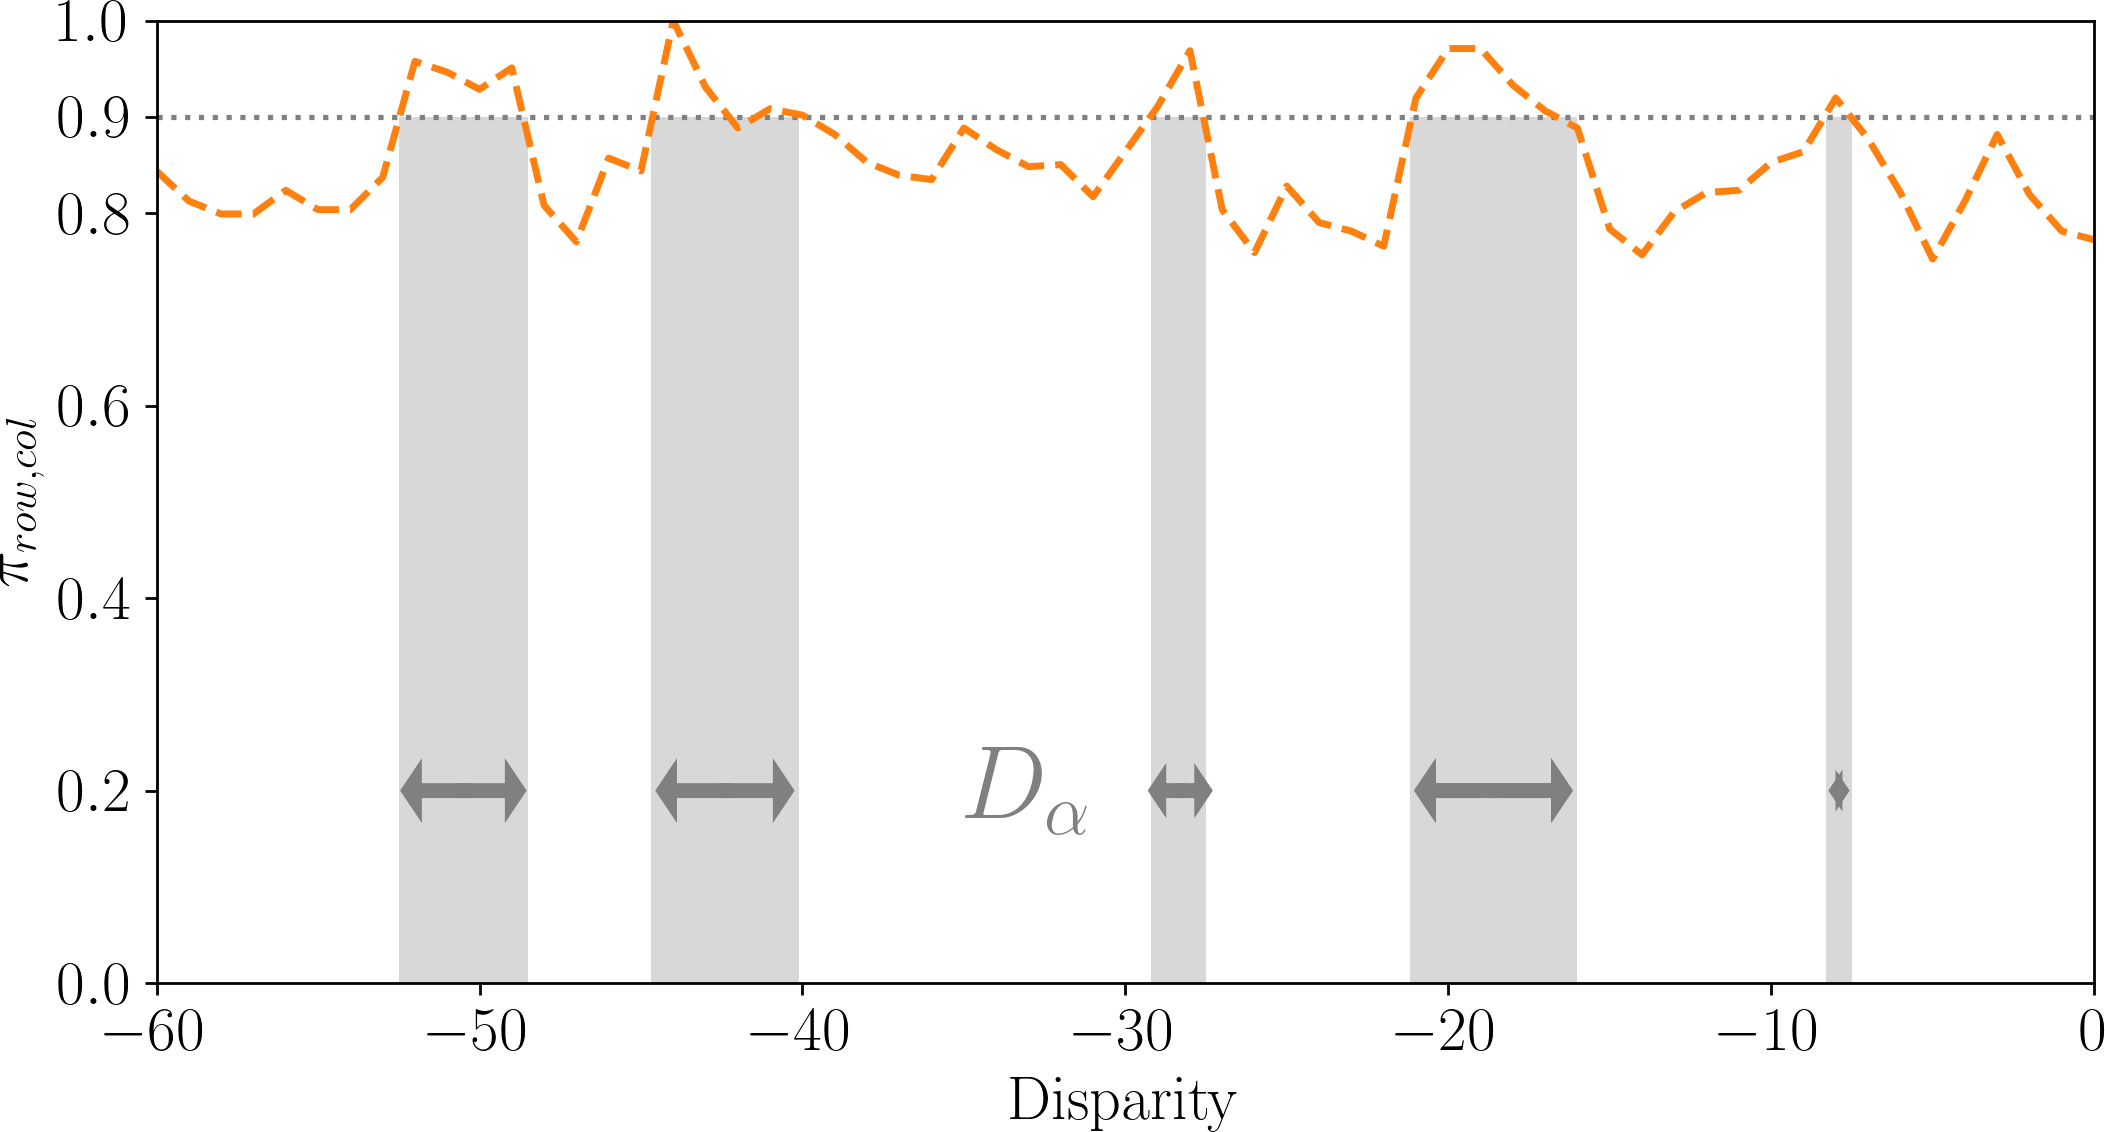
\includegraphics[width=\linewidth]{Images/Chap_5/disparity_interval_2.png}
        \caption{$D_\alpha$ for the orange possibility of \Cref{fig:cost_curves_d}}
        \label{fig:disparity_intervals_b}
    \end{subfigure}
    \begin{subfigure}[t]{0.47\linewidth}
        \centering
        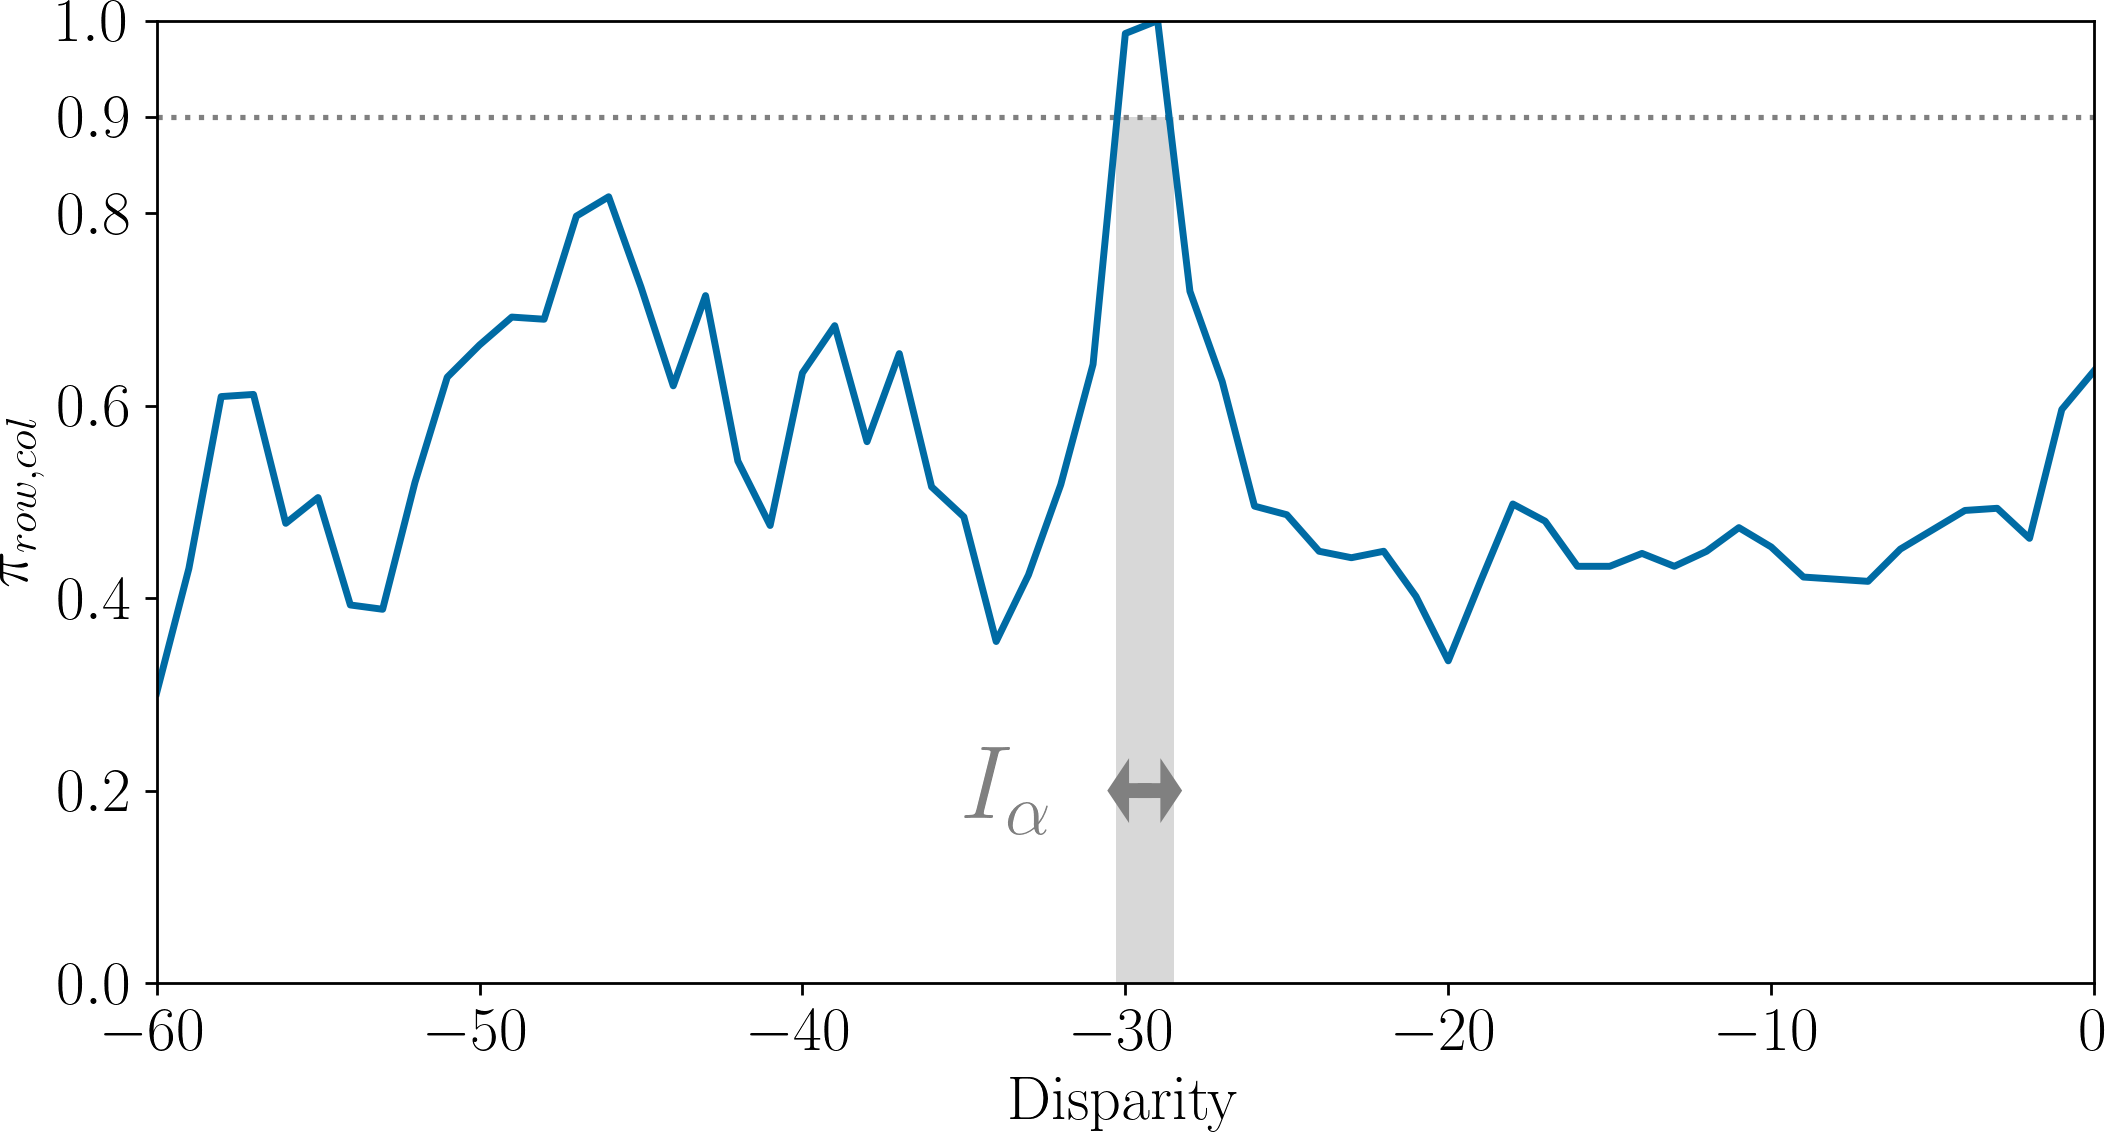
\includegraphics[width=\linewidth]{Images/Chap_5/disparity_interval_3.png}
        \caption{$I_\alpha$ for the blue possibility of \Cref{fig:cost_curves_d}}
        \label{fig:disparity_intervals_c}
    \end{subfigure}\hfill
    \begin{subfigure}[t]{0.47\linewidth}
        \centering
        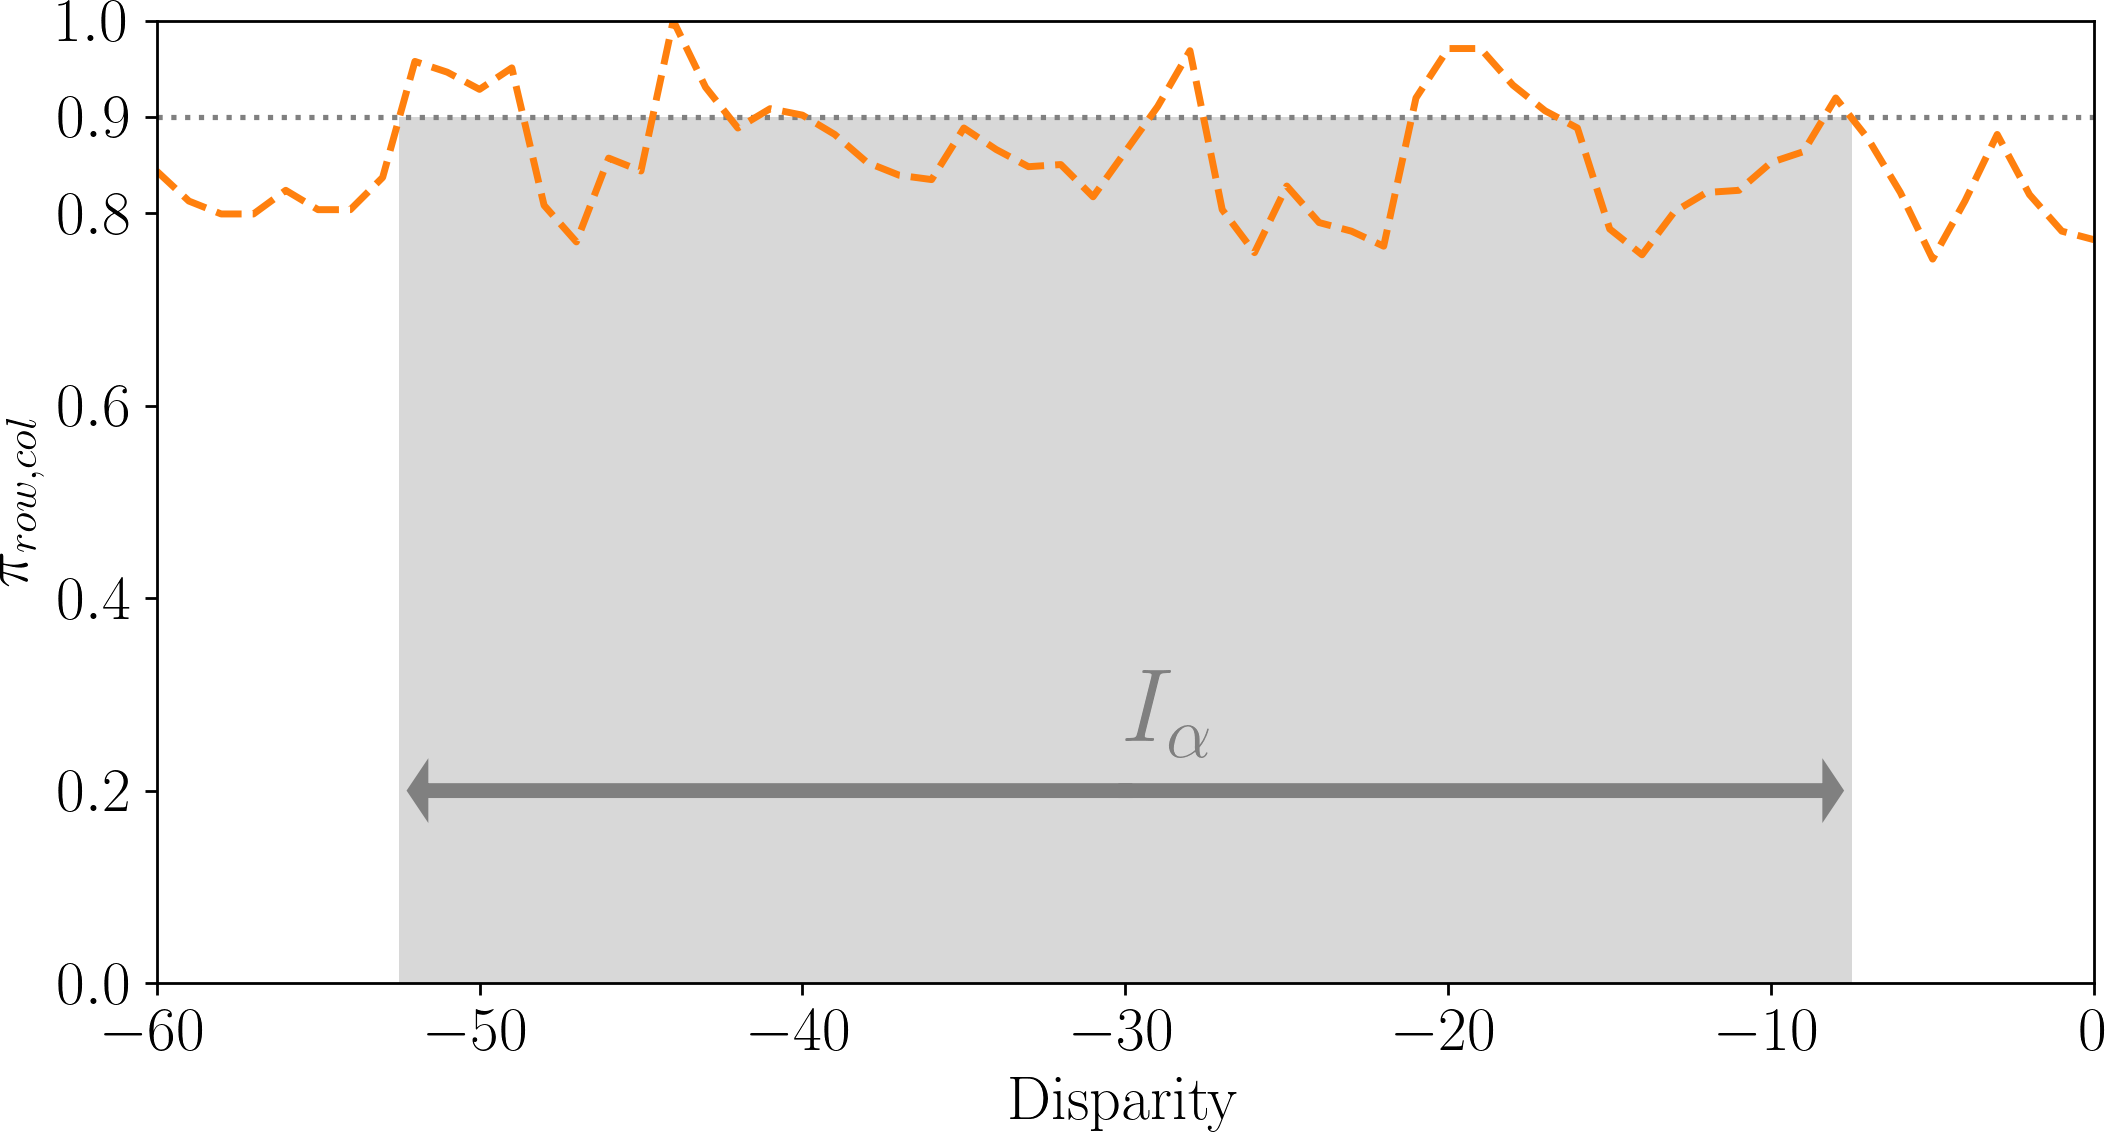
\includegraphics[width=\linewidth]{Images/Chap_5/disparity_interval_4.png}
        \caption{$I_\alpha$ for the orange possibility of \Cref{fig:cost_curves_d}}
        \label{fig:disparity_intervals_d}
    \end{subfigure}\hfill
    \caption{Set of possible disparities $D_\alpha$ and disparity intervals $I_\alpha$ with the same cost curves as in  \Cref{fig:cost_curves_to_possibility}, with $\alpha=0.9$. \Cref{fig:disparity_intervals_a,fig:disparity_intervals_b} represent the set of possible disparities $D_\alpha$ from \cref{eq:set_of_possible_disparities} in gray. \Cref{fig:disparity_intervals_c,fig:disparity_intervals_d} represent disparity intervals $I_\alpha$ from \cref{eq:confidence_disparity_intervals} in gray. There is no difference between $D_\alpha$ and $I_\alpha$ for the blue curve, contrary to the orange dashed curve.}
    \label{fig:disparity_sets_and_intervals}
\end{figure}

\begin{figure}
    \centering
    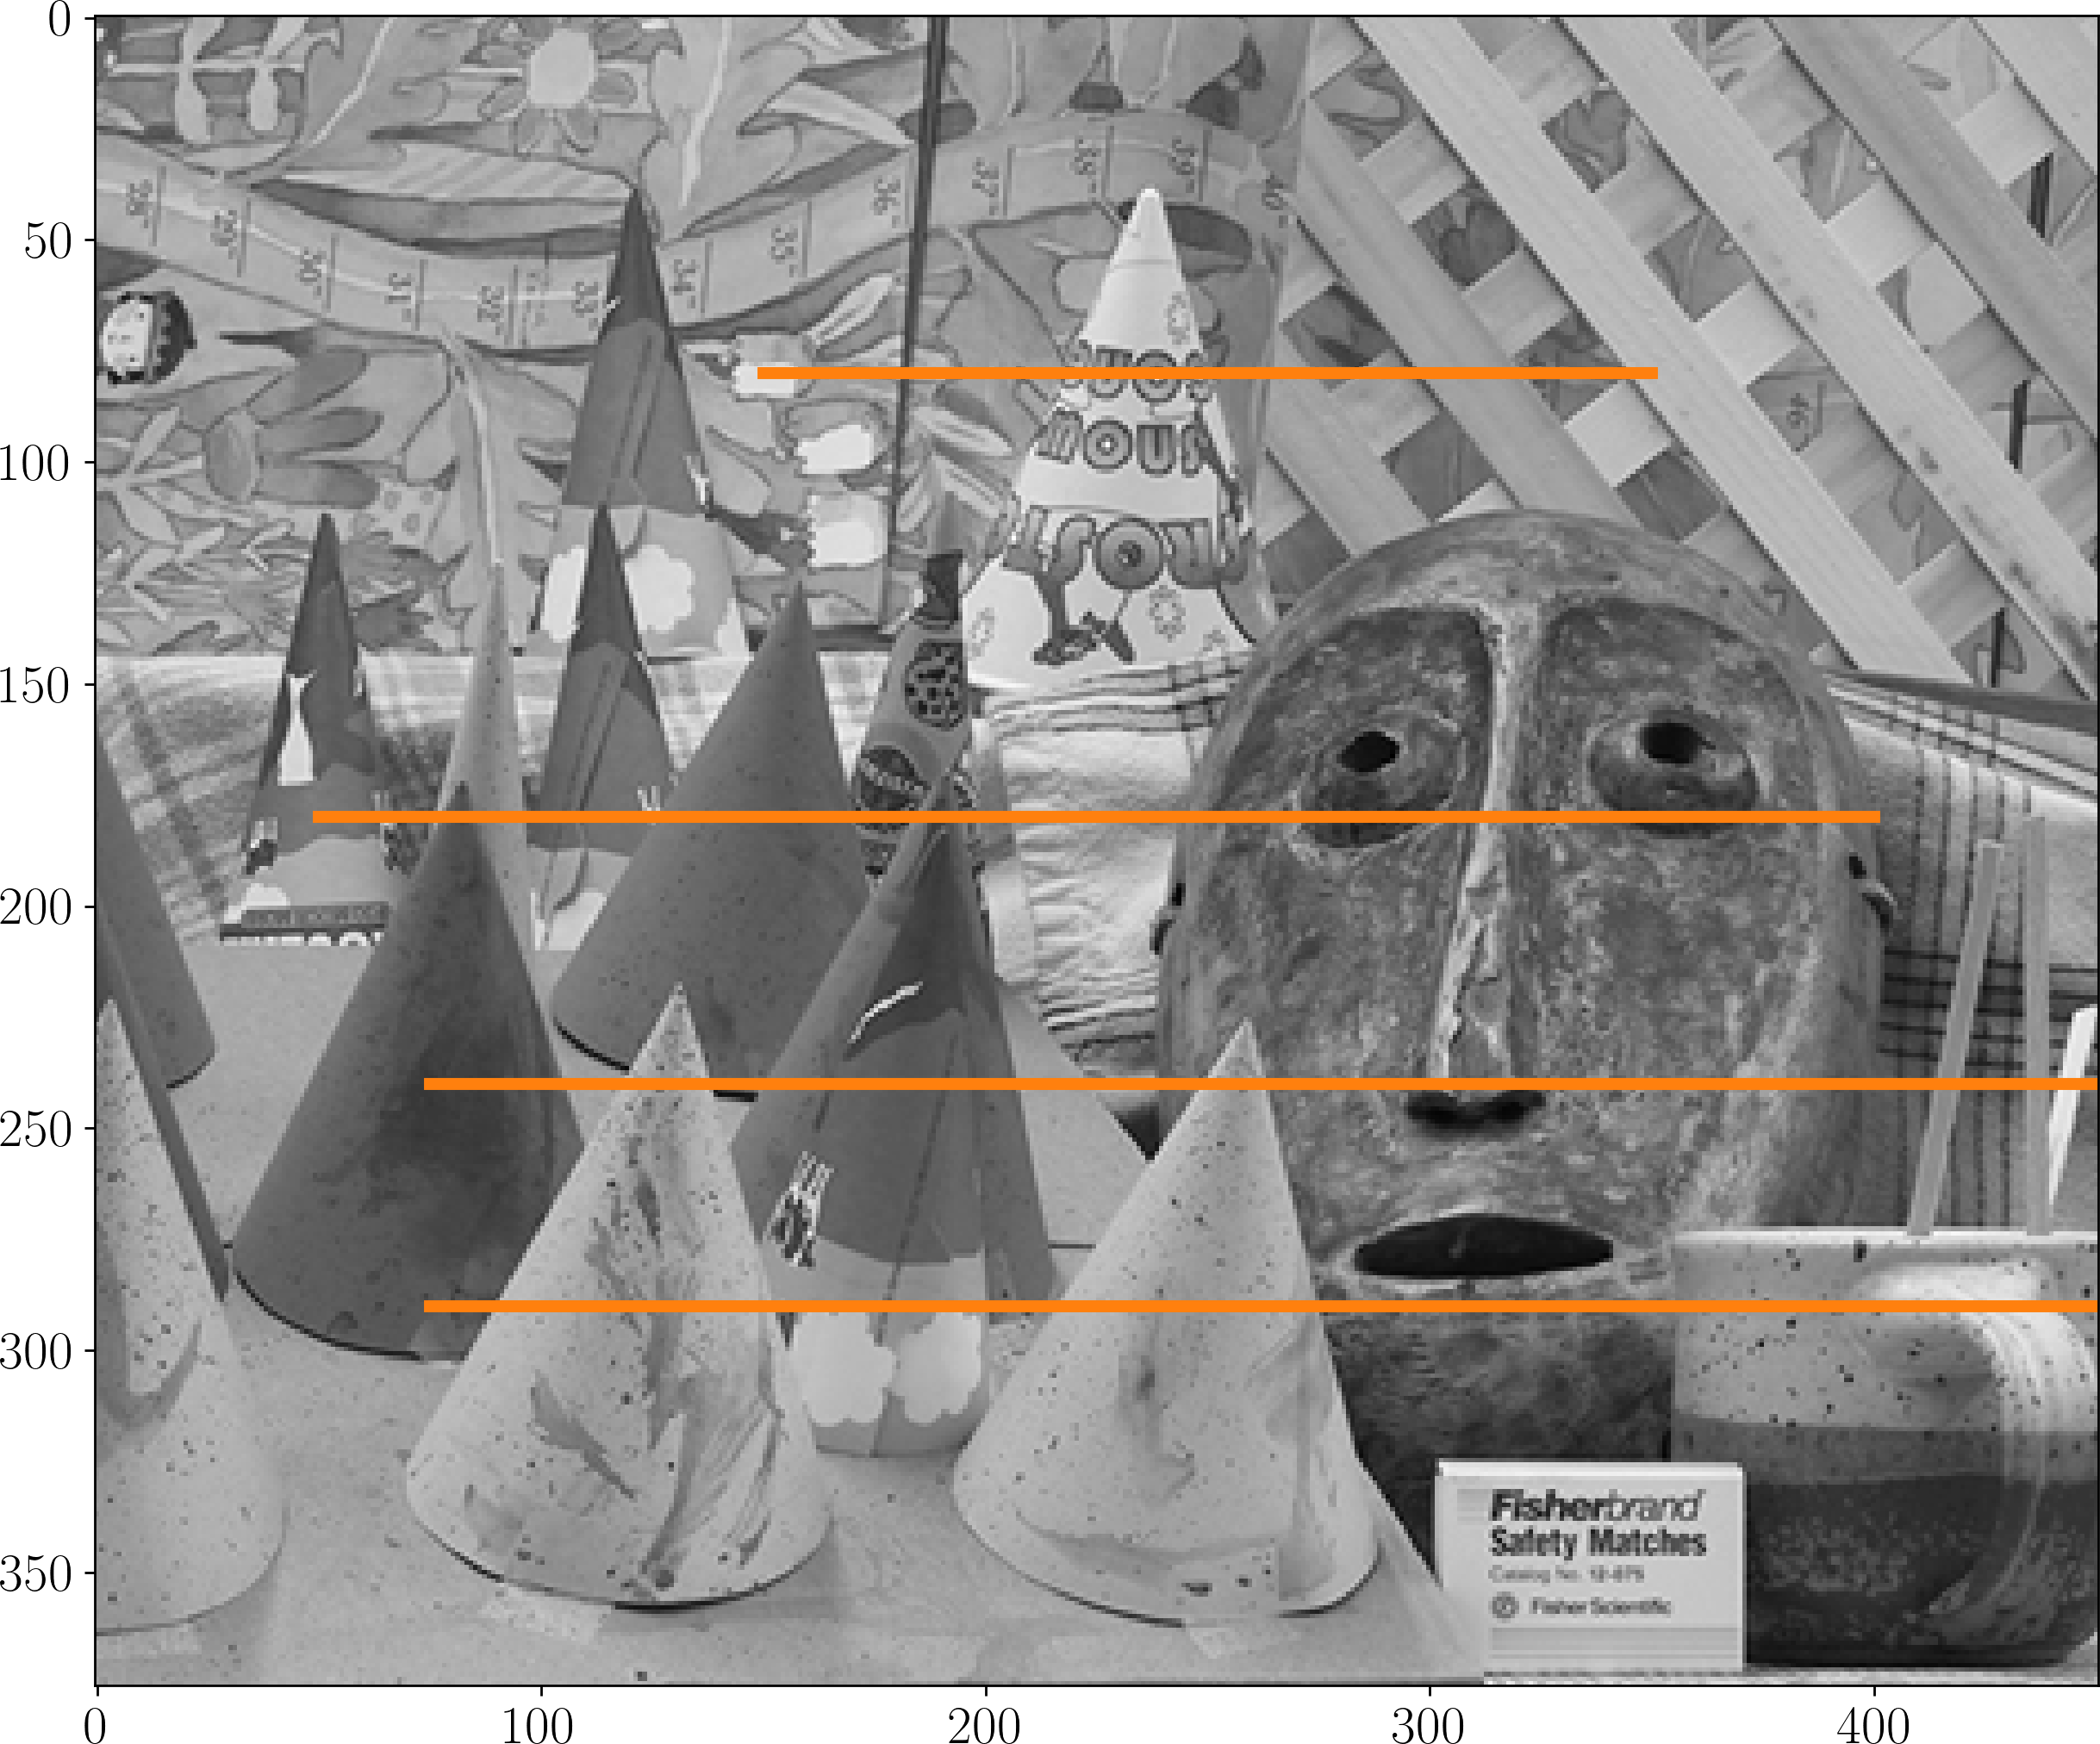
\includegraphics[width=0.5\linewidth]{Images/Chap_5/cones_with_rows.png}
    \caption{Left stereo image from Middlebury Cones. Disparity intervals $I_\alpha$ along orange lines are detailed in \Cref{fig:intervals_ambiguous_row_80,fig:intervals_ambiguous_row_180,fig:intervals_ambiguous_row_240,fig:intervals_ambiguous_row_290}}
    \label{fig:cones_with_rows}
\end{figure}\todoroman{Mettre qu'une seule ligne pour la théorie et rajouter les figures restantes dans la partie résultat}

To qualitatively evaluate the behaviour of disparity confidence intervals $I_\alpha$, we will look at their values for consecutive pixels of the same row. Considered rows\commanue{Rows selected for this analysis?} are presented in \Cref{fig:cones_with_rows}: the upper row ($80$) is smaller than the others so more details can be observed, while other rows allows for a broader view of the intervals\commanue{peut-être préciser si tu as pris les lignes au pif ou non.}.

\begin{figure}
    \centering
    \begin{subfigure}[t]{0.8\linewidth}
        \centering
        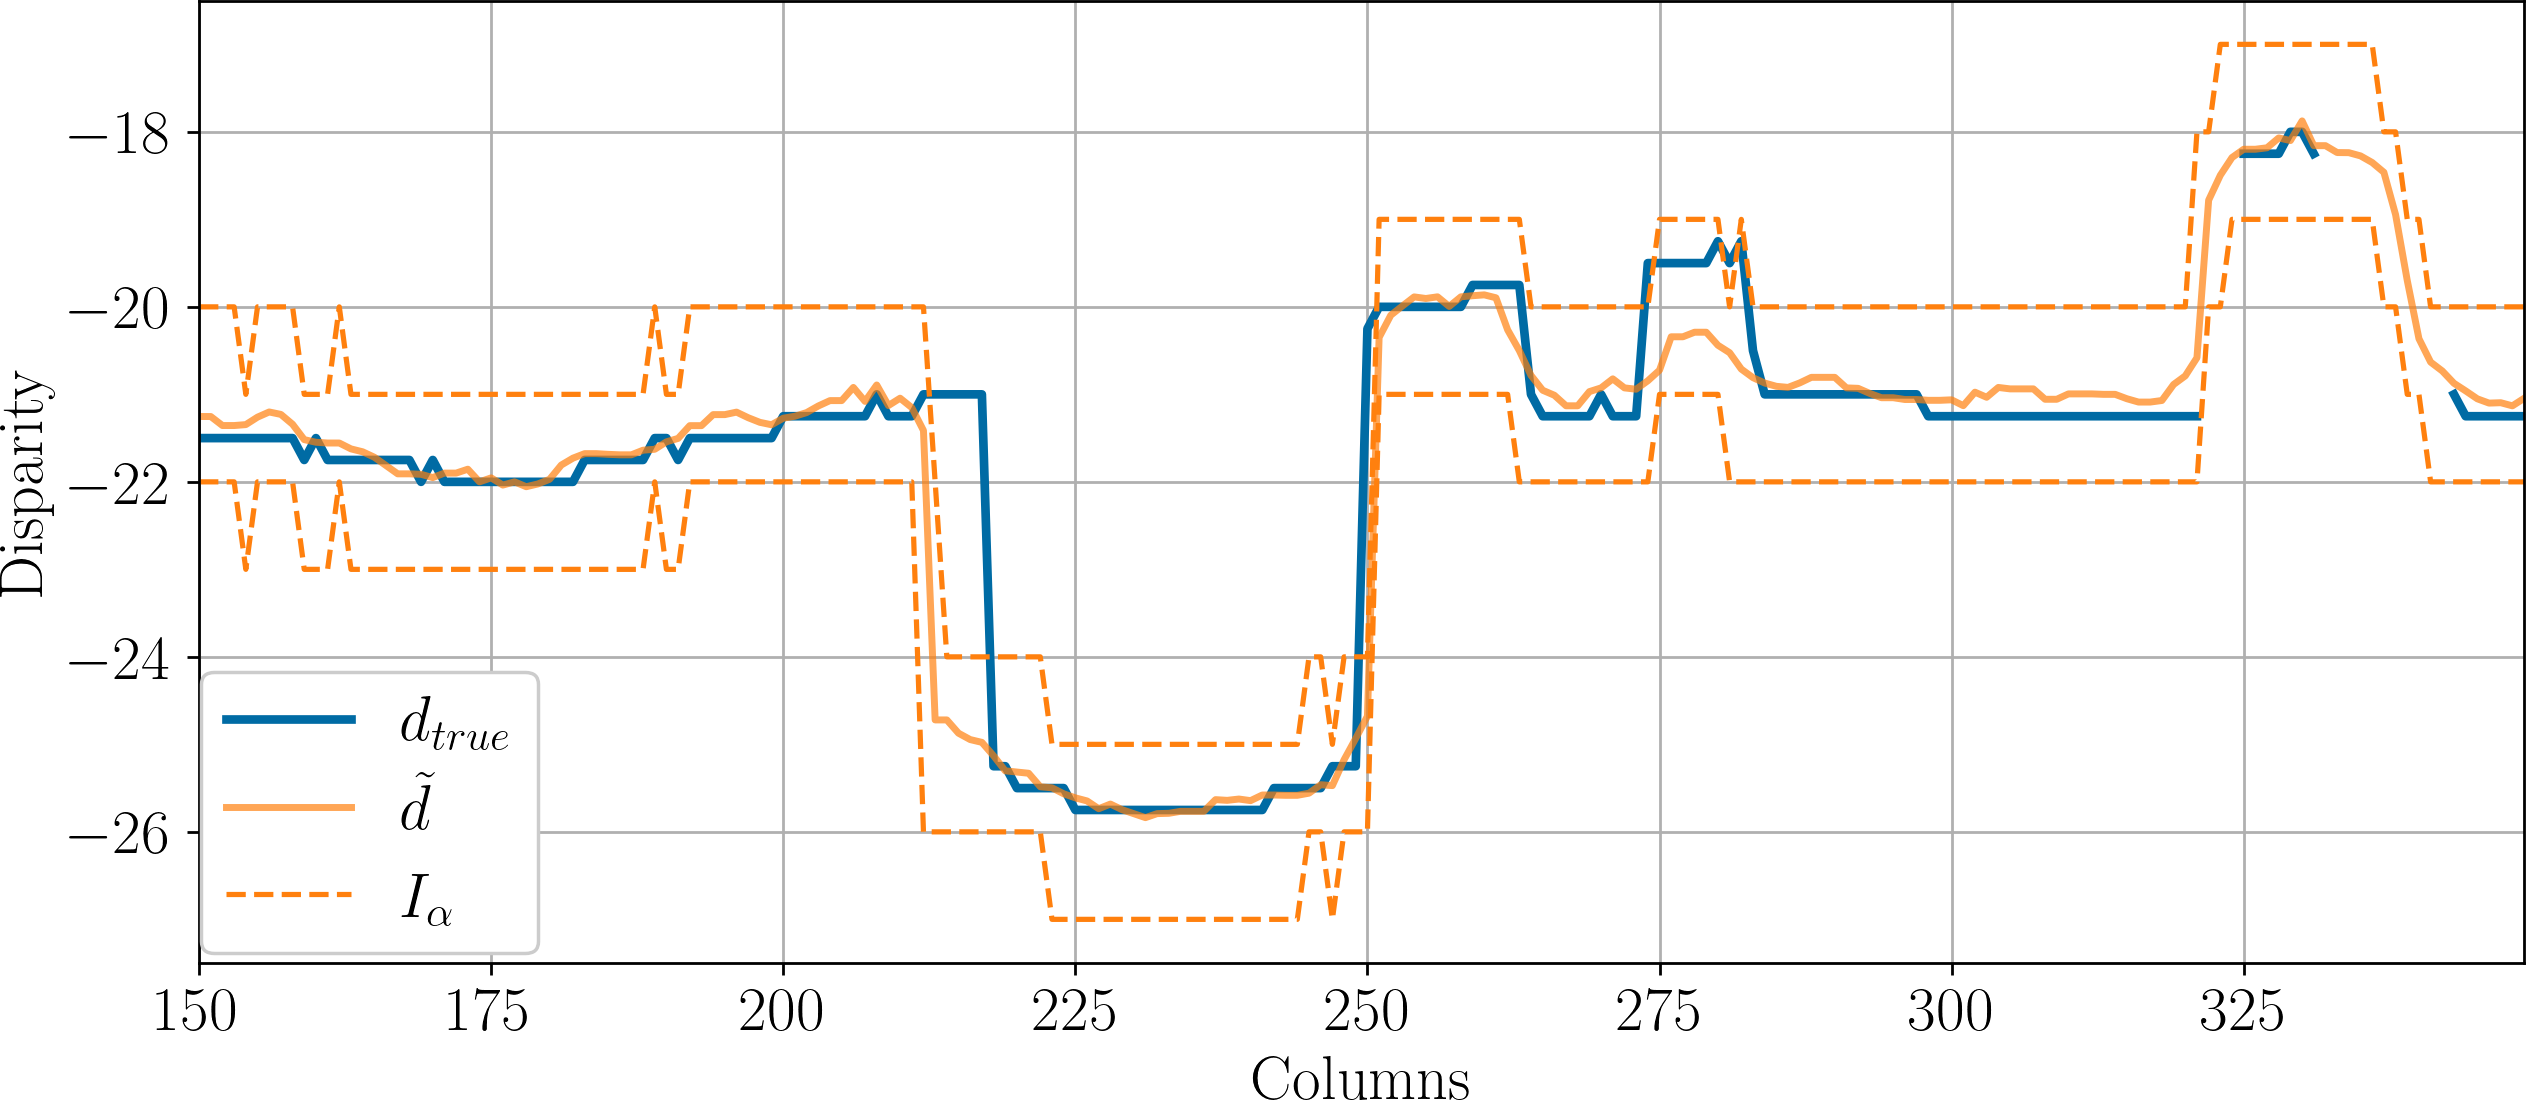
\includegraphics[width=\linewidth]{Images/Chap_5/intervals_ambiguous_area_row_80_1.png}
        \caption{$I_\alpha$ without regularization in low confidence areas}
        \label{fig:intervals_ambiguous_row_80_1}
    \end{subfigure}\hfill
    \begin{subfigure}[t]{0.8\linewidth}
        \centering
        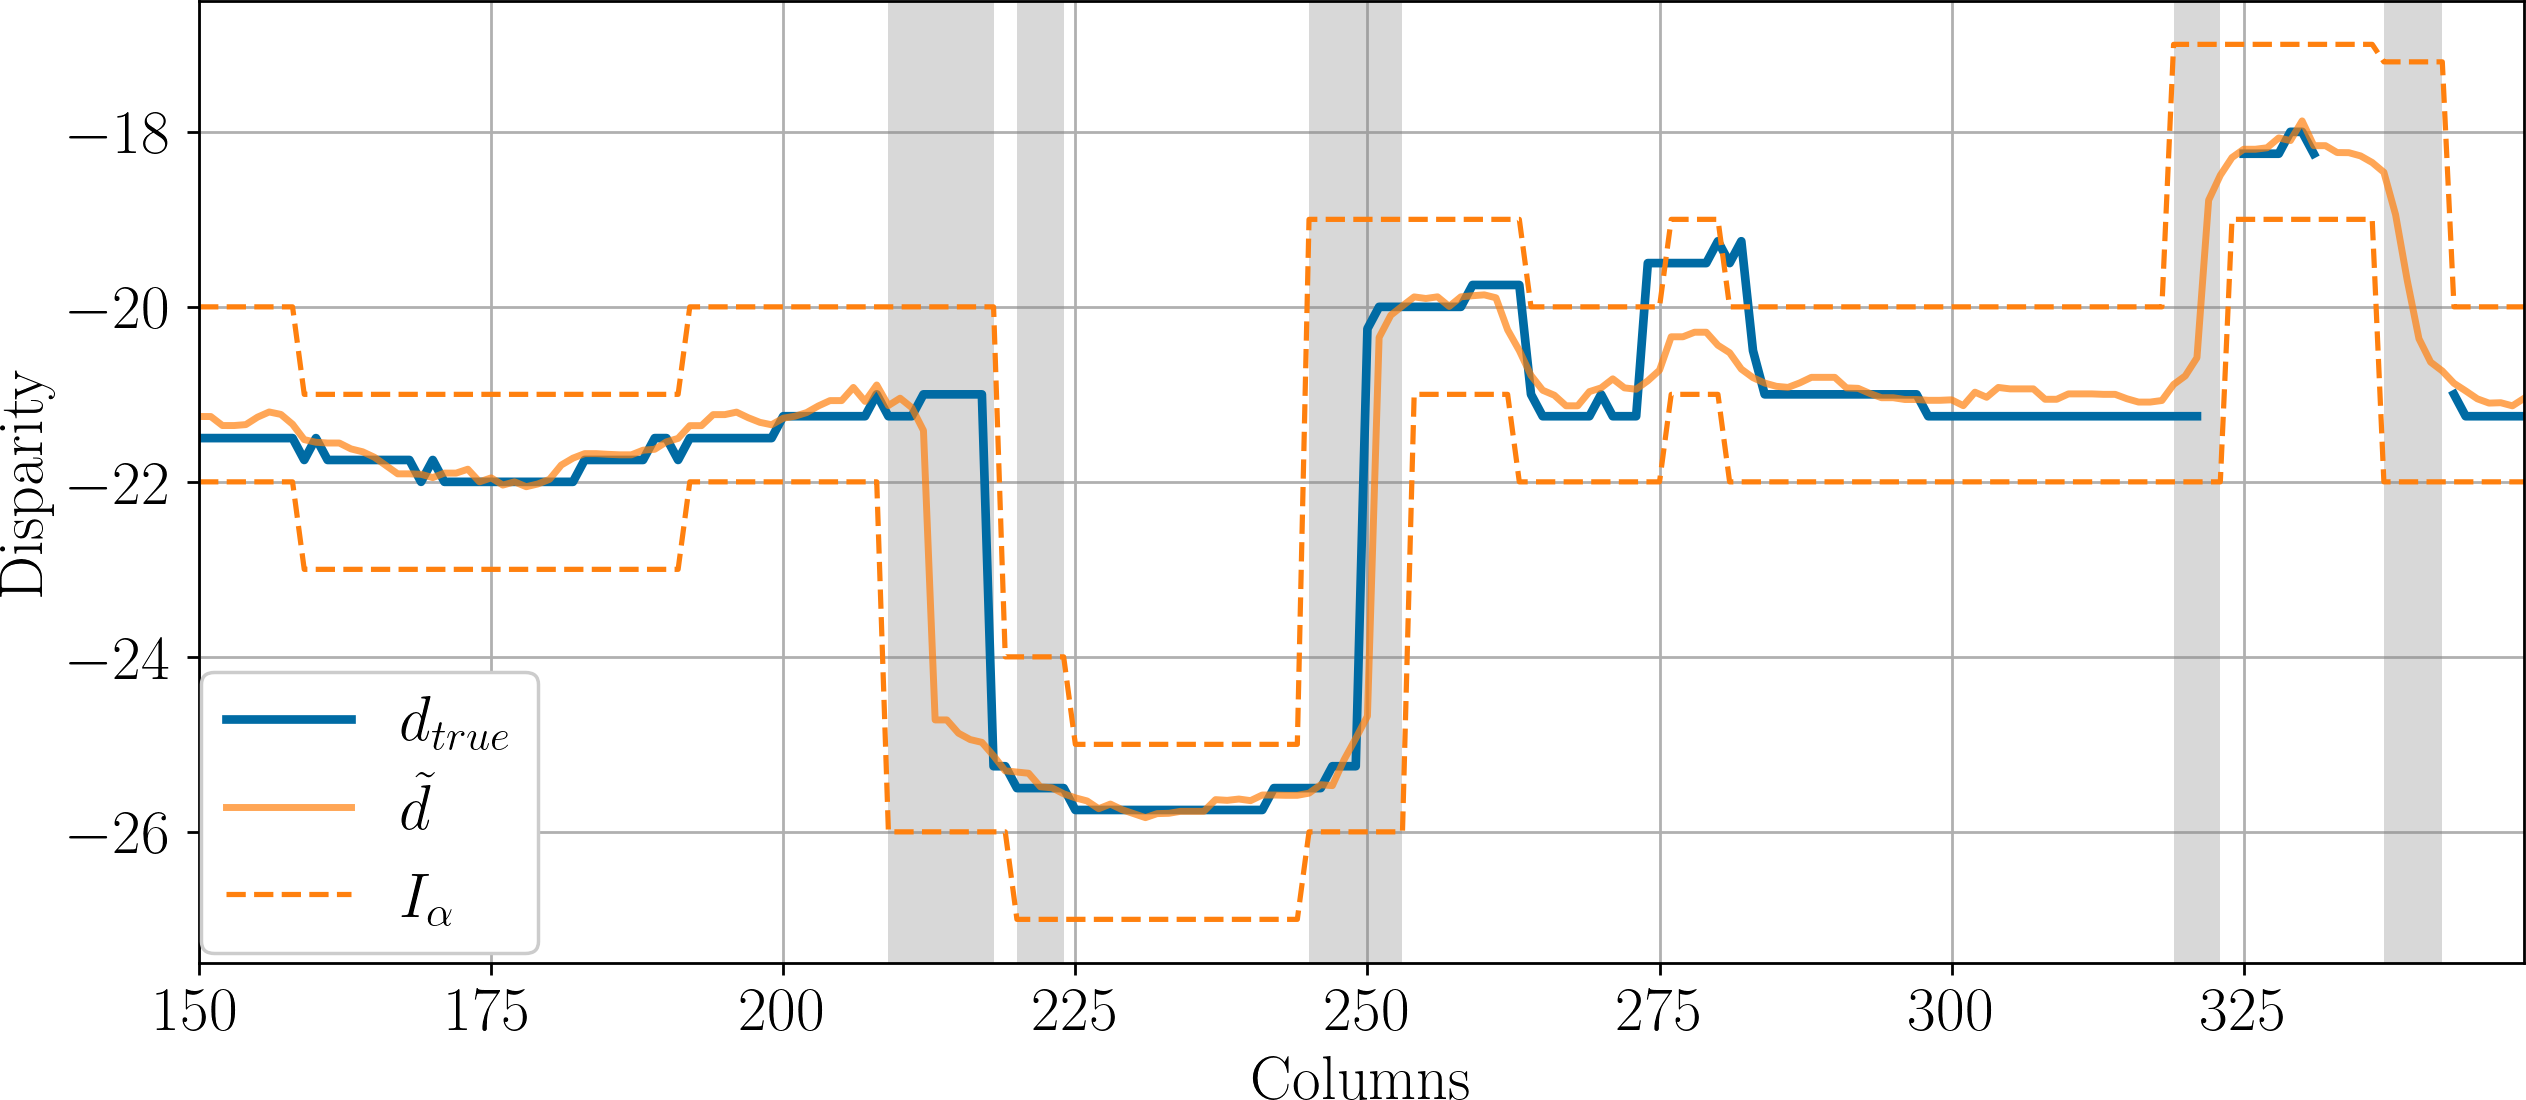
\includegraphics[width=\linewidth]{Images/Chap_5/intervals_ambiguous_area_row_80_2.png}
        \caption{$I_\alpha$ with regularization in low confidence areas}
        \label{fig:intervals_ambiguous_row_80_2}
    \end{subfigure}
    \caption{$I_\alpha$ with and without regularization in low confidence area, for row $80$ of the image of \Cref{fig:cones_with_rows}. Low confidence areas are indicated by the gray areas.}
    \label{fig:intervals_ambiguous_row_80}
\end{figure}
\begin{figure}
    \centering
    \begin{subfigure}[t]{\linewidth}
        \centering
        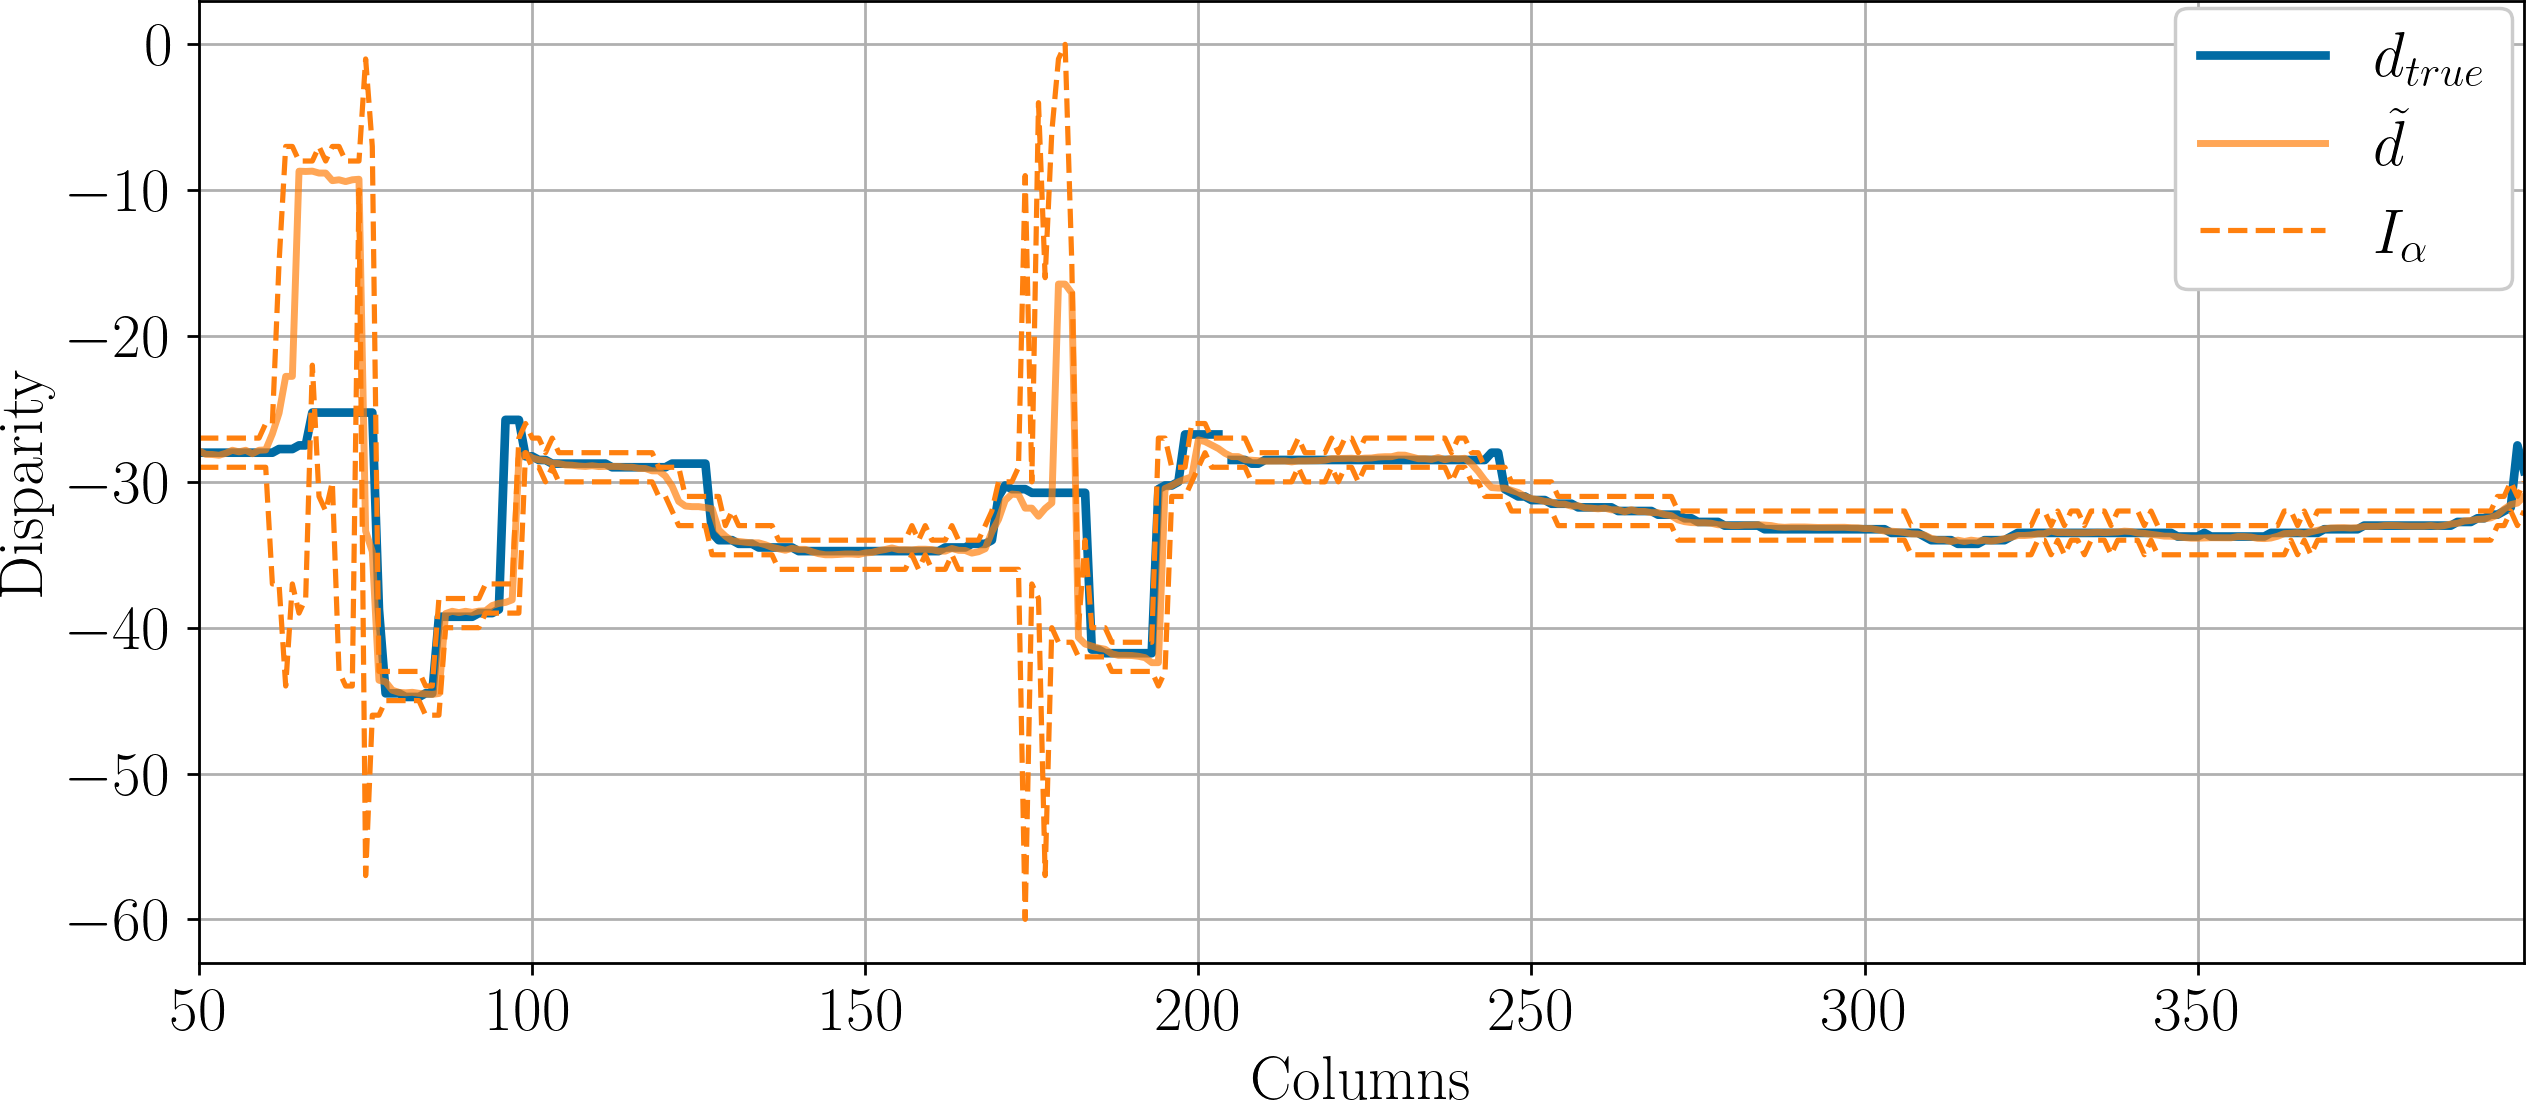
\includegraphics[width=\linewidth]{Images/Chap_5/intervals_ambiguous_area_row_180_1.png}
        \caption{$I_\alpha$ without regularization in low confidence areas}
        \label{fig:intervals_ambiguous_row_180_1}
    \end{subfigure}\hfill
    \begin{subfigure}[t]{\linewidth}
        \centering
        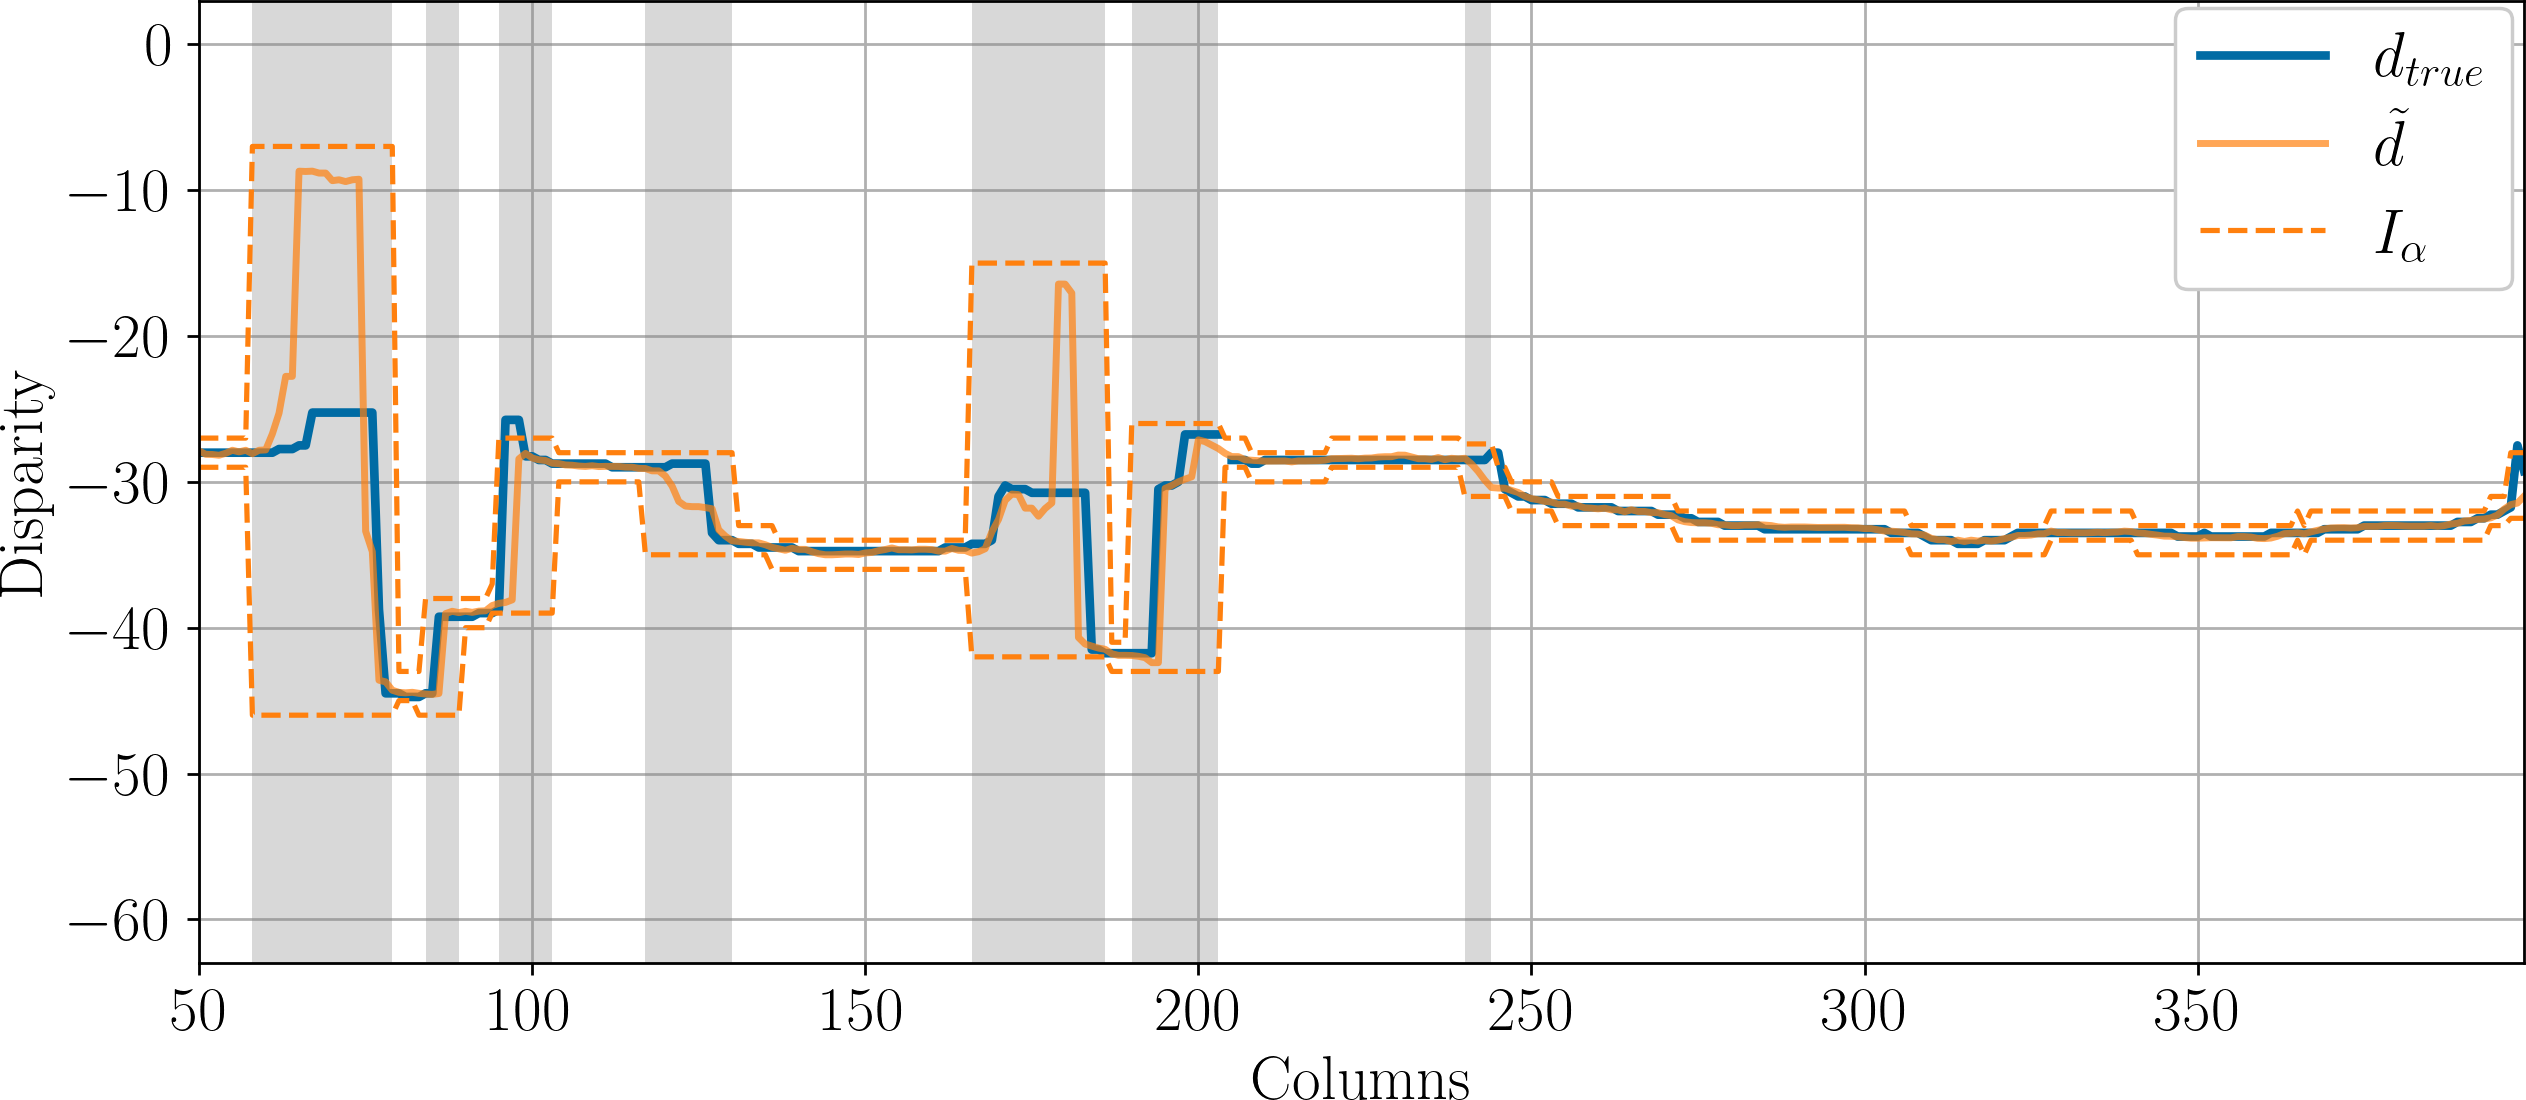
\includegraphics[width=\linewidth]{Images/Chap_5/intervals_ambiguous_area_row_180_2.png}
        \caption{$I_\alpha$ with regularization in low confidence areas}
        \label{fig:intervals_ambiguous_row_180_2}
    \end{subfigure}
    \caption{$I_\alpha$ with and without regularization in low confidence area, for row $180$ of the image of \Cref{fig:cones_with_rows}. Low confidence areas are indicated by the gray areas.}
    \label{fig:intervals_ambiguous_row_180}
\end{figure}

By construction, $I_\alpha$ will always contain the predicted disparity $\tilde{d}$ as the maximum of each possibility curve will also be selected as the predicted disparity by winner-takes-all strategy. However, We are interested to see if intervals can contain the true disparity $d_{true}$ even when the predicted disparity is far from it. \Cref{fig:intervals_ambiguous_row_80_1,fig:intervals_ambiguous_row_180_1,fig:intervals_ambiguous_row_240_1,fig:intervals_ambiguous_row_290_1} represent the disparity intervals $I_\alpha$, predicted disparity $\tilde{d}$ and true disparity $d_{true}$ for the different rows. A first observation is that intervals correctly contain the true disparity in regions were there are no strong variations of disparities. In  \Cref{fig:intervals_ambiguous_row_180_1}, the intervals in columns $50$ to $75$ and around $175$ are much larger than in the rest of the figure. In those areas, the predicted disparity is also far from the ground truth. This translates the fact that the method for creating intervals is able to detect the difficulties encountered by the correlator when predicting a disparity, and to adapt the intervals size consequently. On the downside, we can see that near strong variations of the disparity, the intervals tend to ``miss'' the discontinuities. Indeed, they do not contain the true disparity around those areas, as observed near columns $215$ and $250$ of \Cref{fig:intervals_ambiguous_row_80_1}, columns $95$, $125$ of \Cref{fig:intervals_ambiguous_row_180_1}, columns $100$, $115$, $150$, $200$, $250$ of \Cref{fig:intervals_ambiguous_row_240_1} 
and finally columns $90$, $200$ and $210$ of \Cref{fig:intervals_ambiguous_row_290_1}. The intervals and gray area presented in \Cref{fig:intervals_ambiguous_row_80_2,fig:intervals_ambiguous_row_180_2,fig:intervals_ambiguous_row_240_2,fig:intervals_ambiguous_row_290_2} will be explained in \Cref{sec:regularization_of_intervals}.

The method presented in this section seems to offer a good estimation of the error in the disparity estimation step. Some errors remain near disparity discontinuities, which we will try to rectify in \Cref{sec:regularization_of_intervals}.

\begin{figure}
    \centering
    \begin{subfigure}[t]{\linewidth}
        \centering
        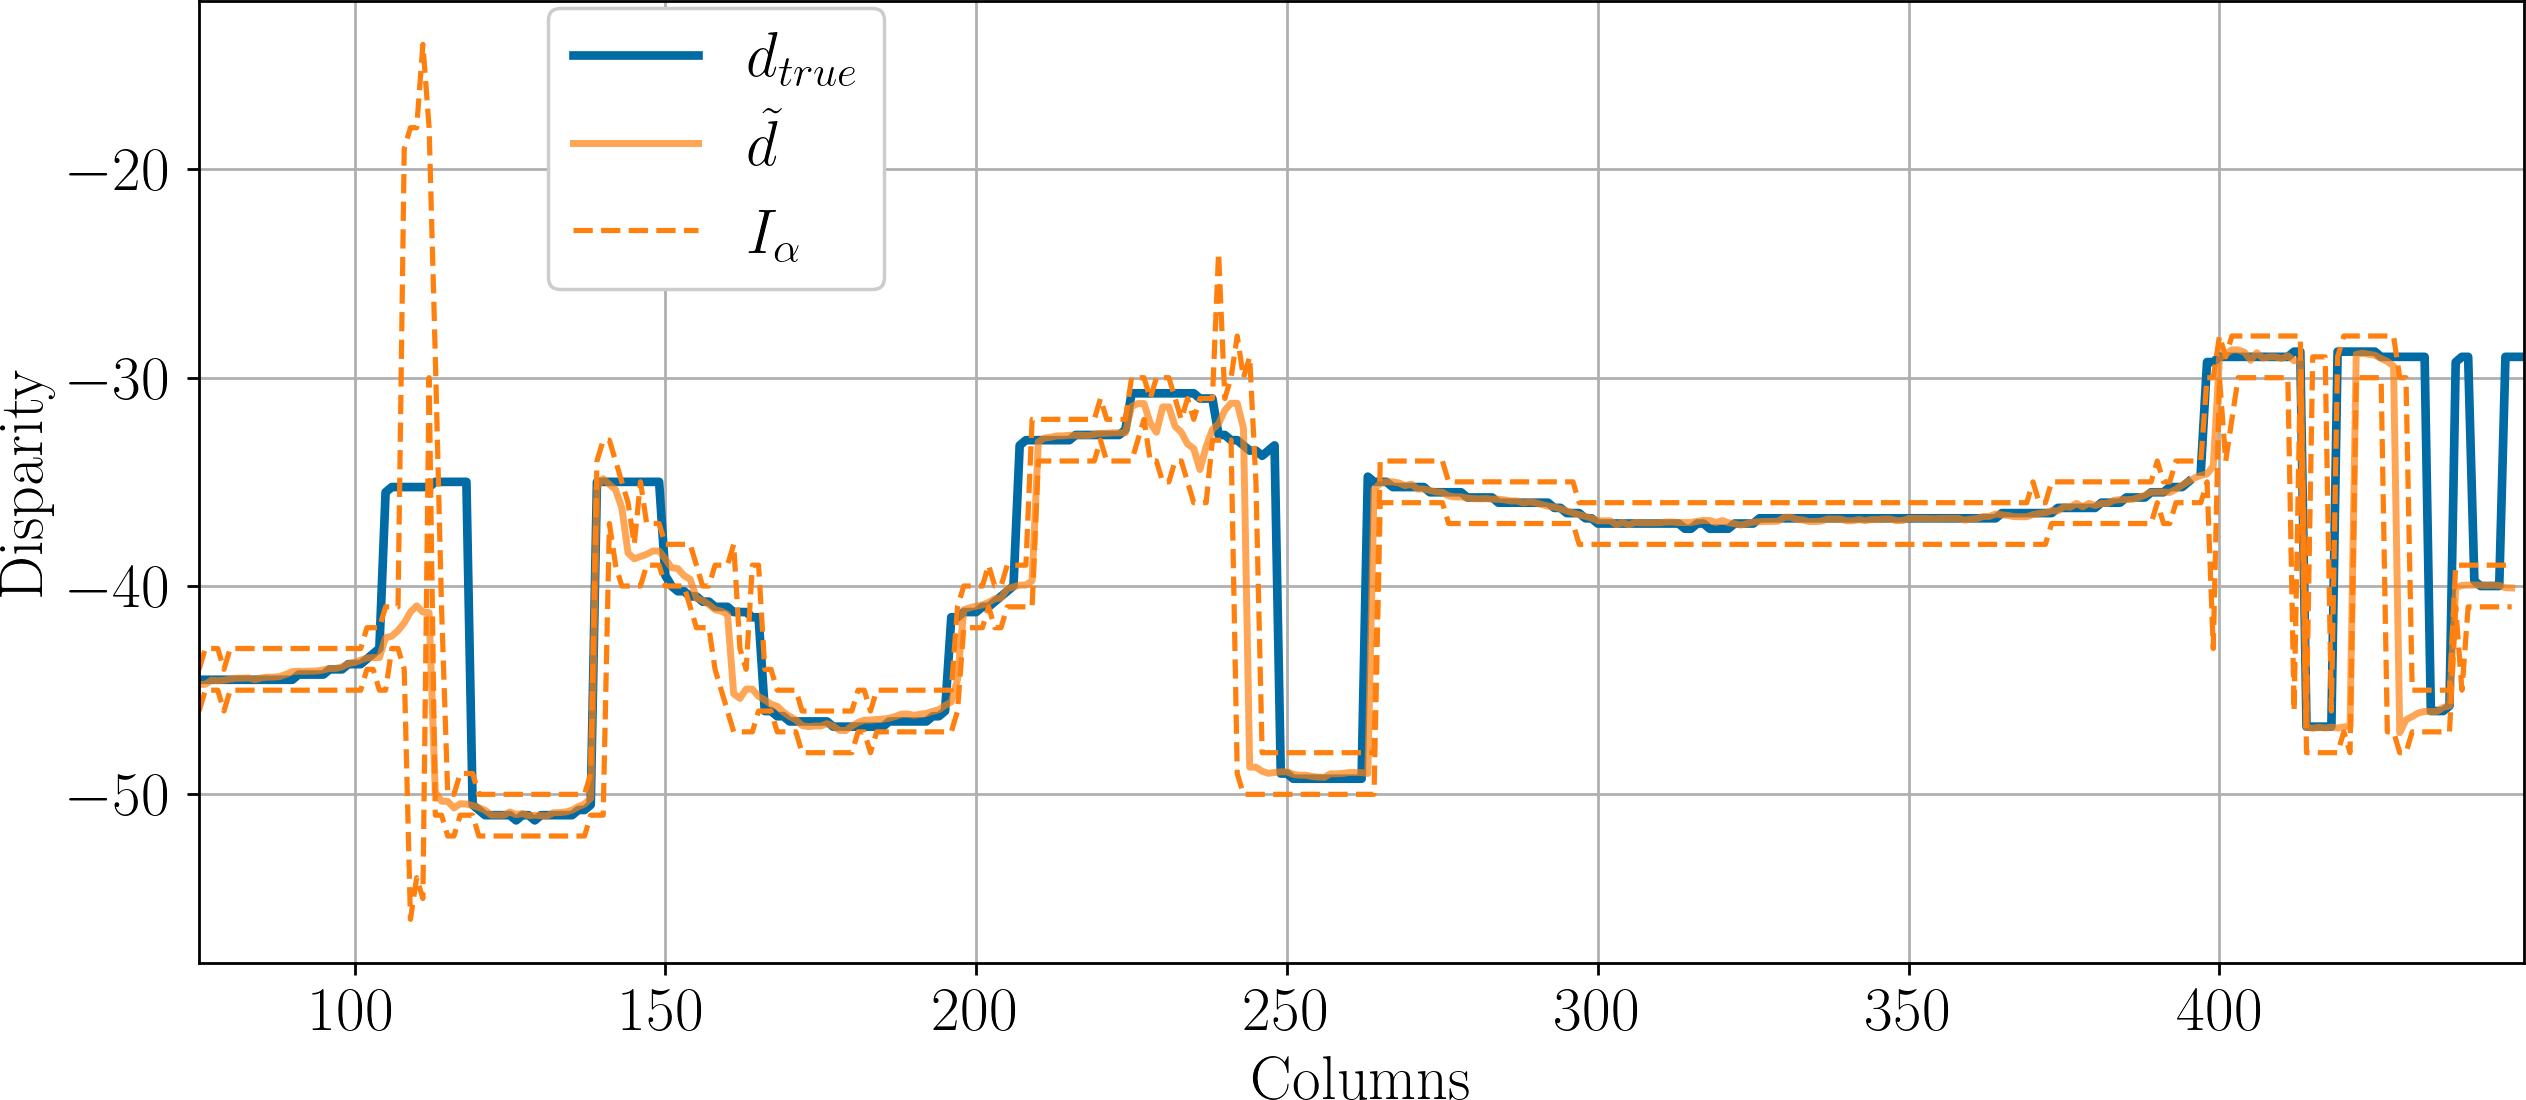
\includegraphics[width=\linewidth]{Images/Chap_5/intervals_ambiguous_area_row_240_1.png}
        \caption{$I_\alpha$ without regularization in low confidence areas}
        \label{fig:intervals_ambiguous_row_240_1}
    \end{subfigure}\hfill
    \begin{subfigure}[t]{\linewidth}
        \centering
        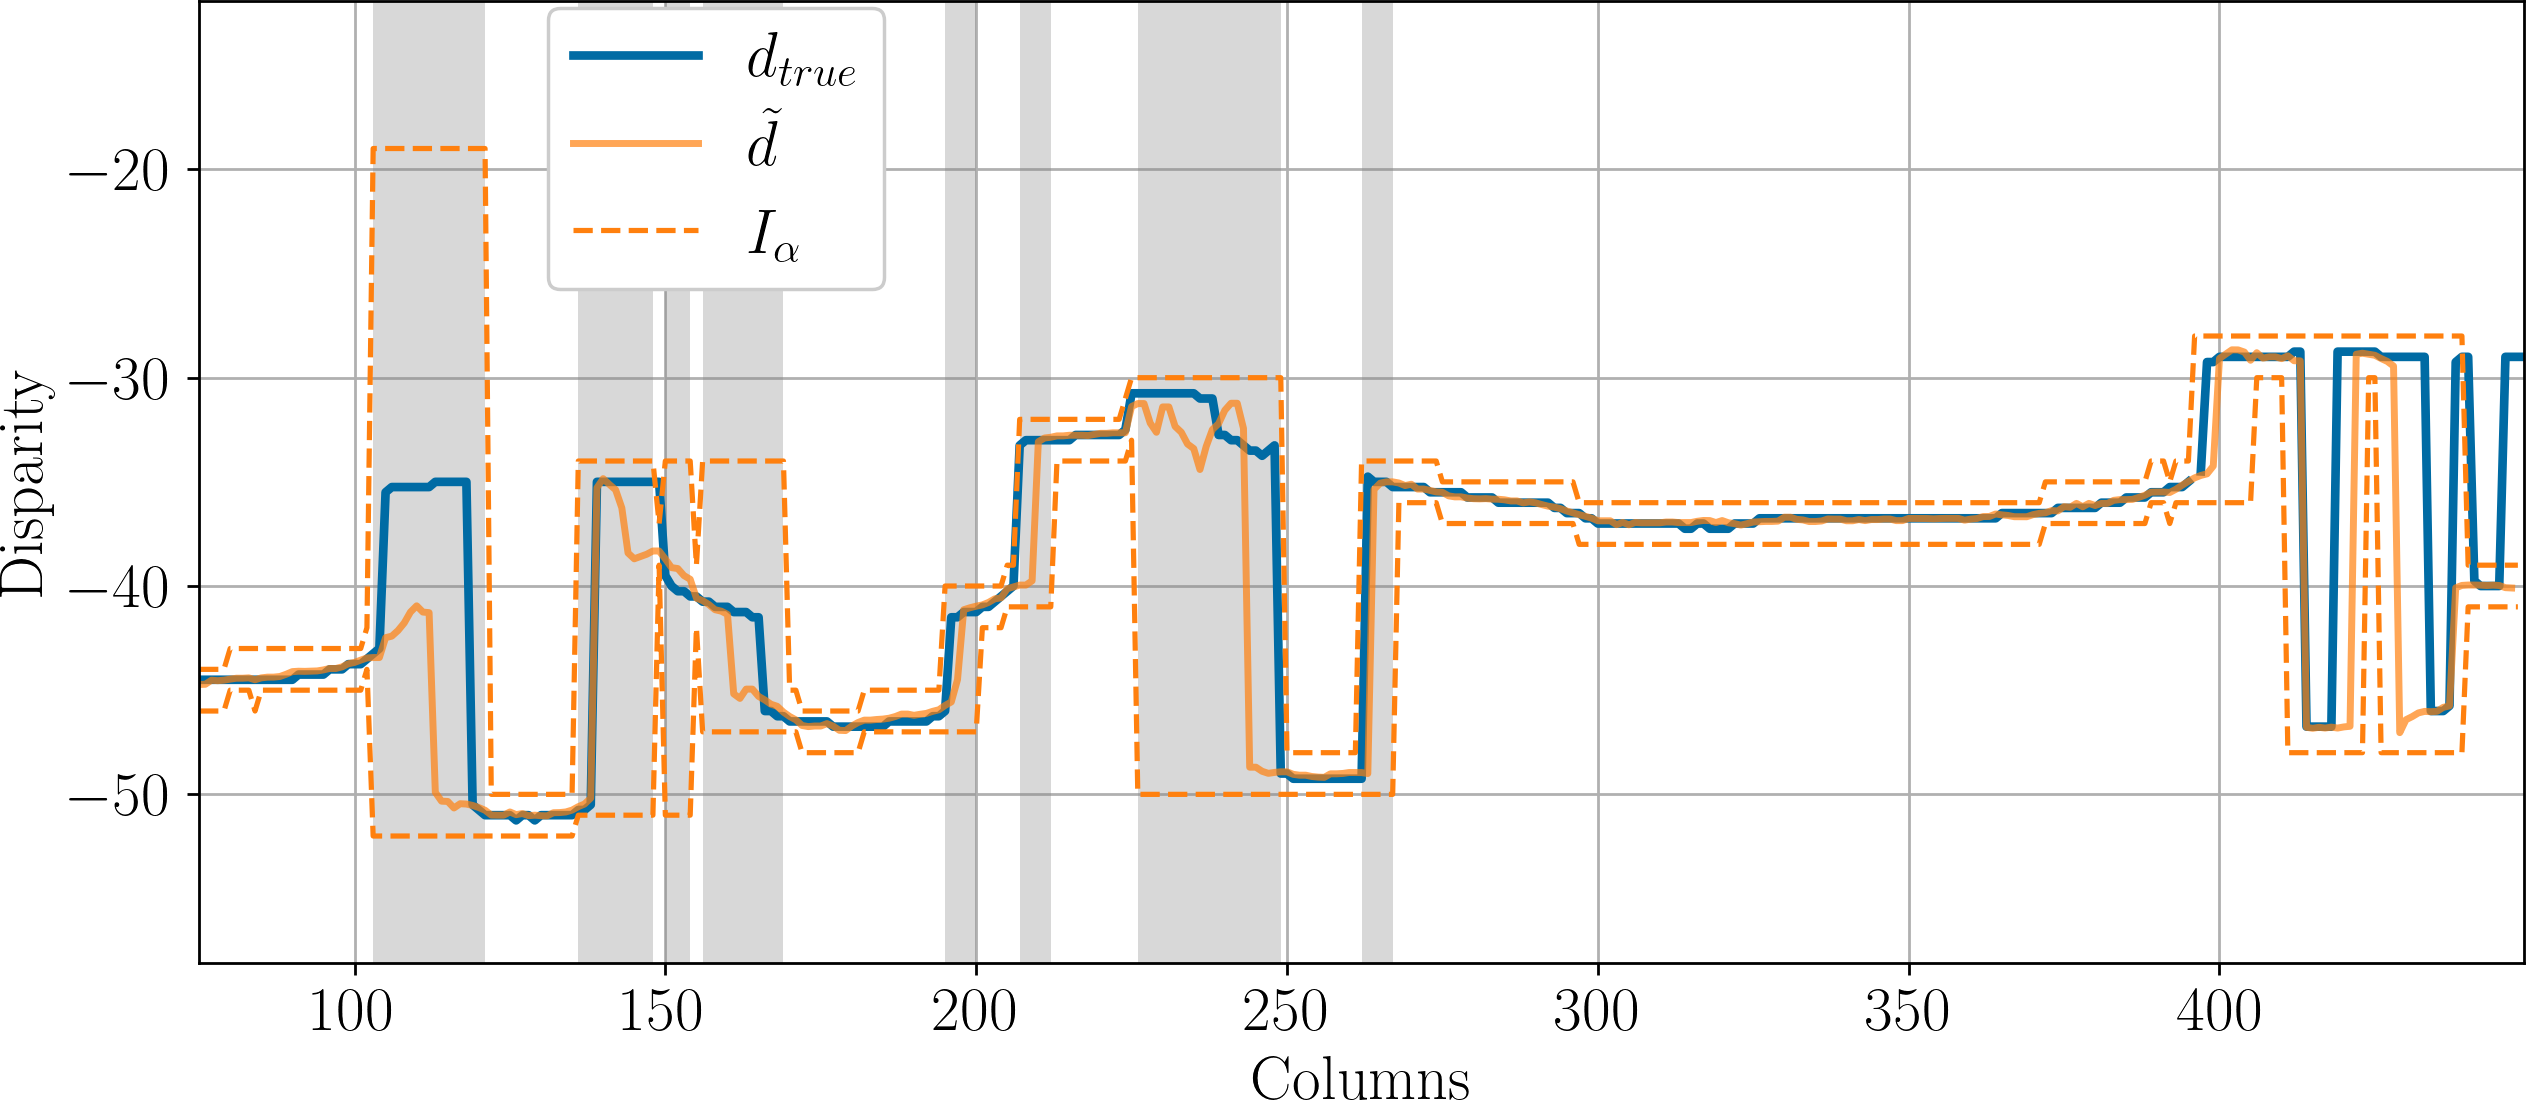
\includegraphics[width=\linewidth]{Images/Chap_5/intervals_ambiguous_area_row_240_2.png}
        \caption{$I_\alpha$ with regularization in low confidence areas}
        \label{fig:intervals_ambiguous_row_240_2}
    \end{subfigure}
    \caption{$I_\alpha$ with and without regularization in low confidence area, for row $240$ of the image of \Cref{fig:cones_with_rows}. Low confidence areas are indicated by the gray areas.}\commanue{bah j'avoue que c'est bizarre d'avoir ici les courbes avace regularisation dans les zones peu confiante vu que maintenant tu en parles bcp plus loin.}
    \label{fig:intervals_ambiguous_row_240}
\end{figure}

\begin{figure}
    \centering
    \begin{subfigure}[t]{\linewidth}
        \centering
        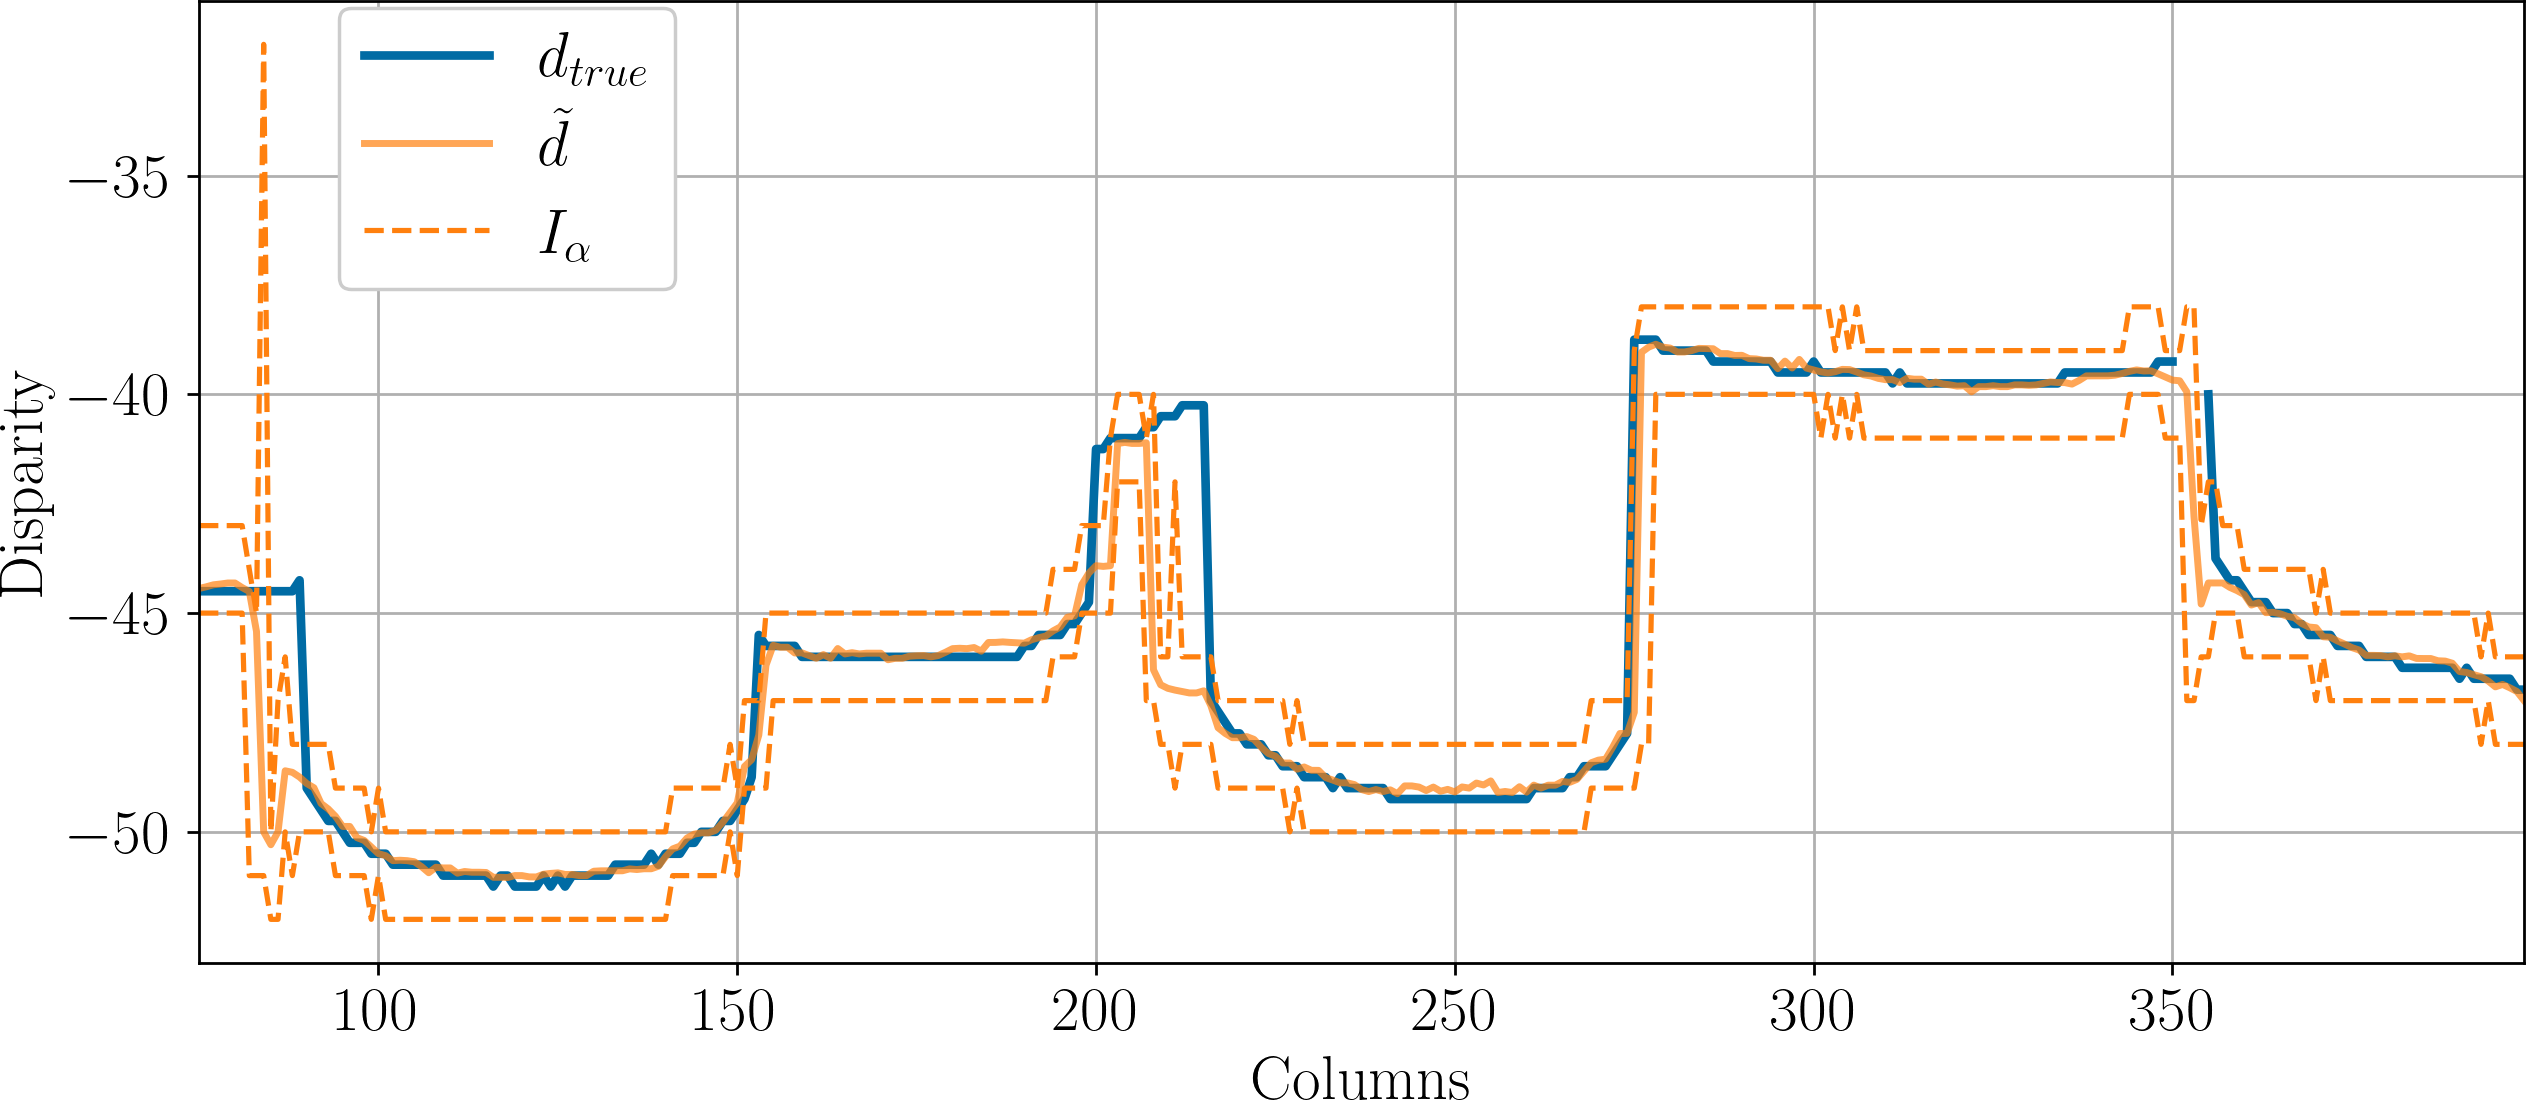
\includegraphics[width=\linewidth]{Images/Chap_5/intervals_ambiguous_area_row_290_1.png}
        \caption{$I_\alpha$ without regularization in low confidence areas}
        \label{fig:intervals_ambiguous_row_290_1}
    \end{subfigure}\hfill
    \begin{subfigure}[t]{\linewidth}
        \centering
        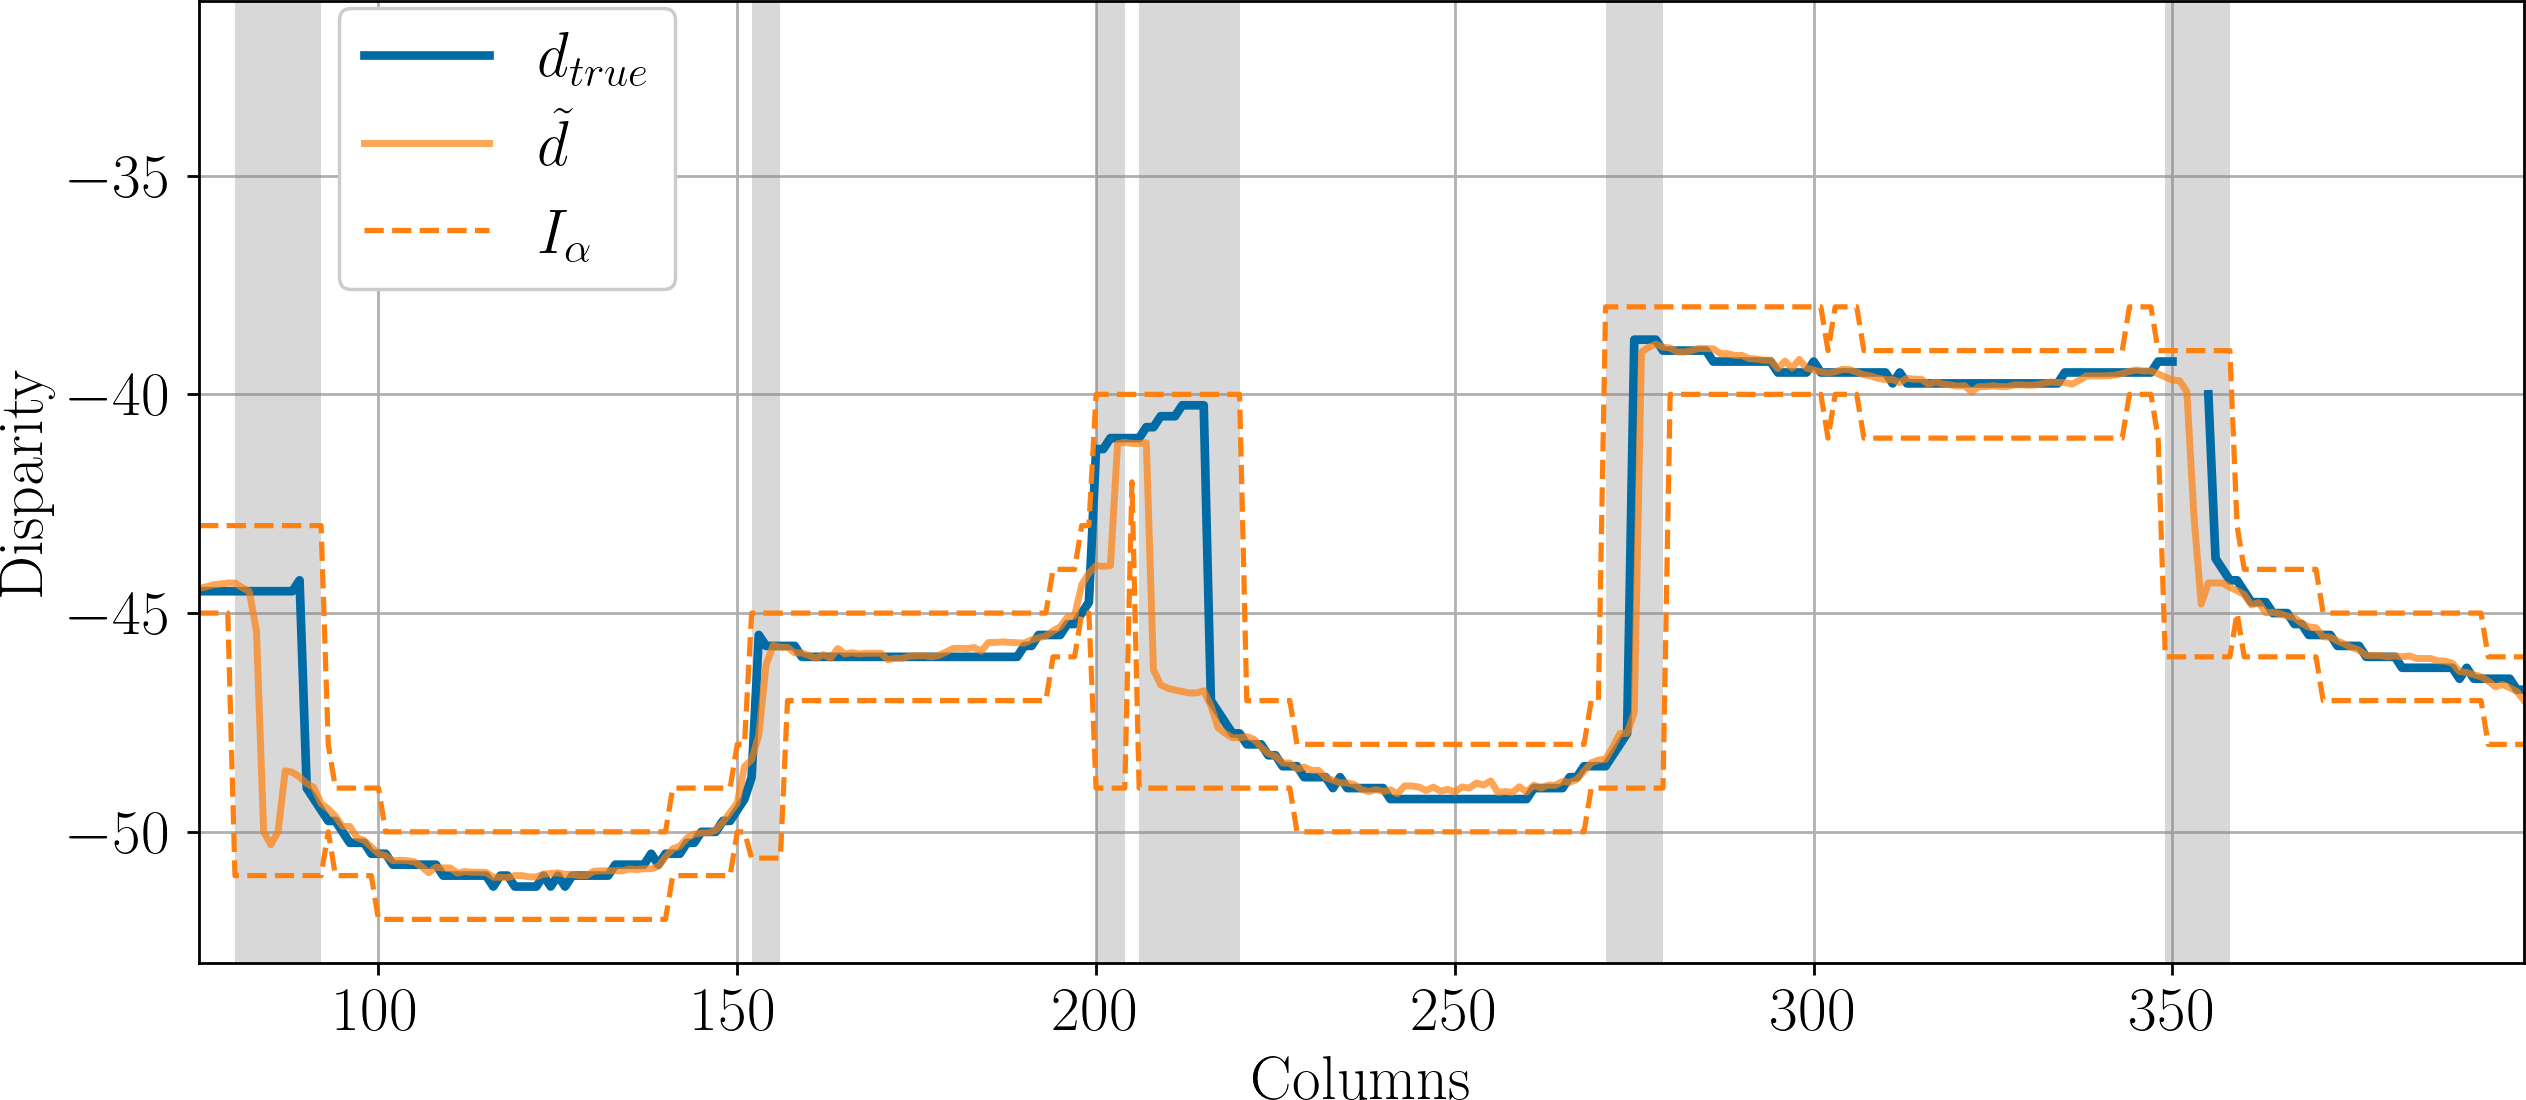
\includegraphics[width=\linewidth]{Images/Chap_5/intervals_ambiguous_area_row_290_2.png}
        \caption{$I_\alpha$ with regularization in low confidence areas}
        \label{fig:intervals_ambiguous_row_290_2}
    \end{subfigure}
    \caption{$I_\alpha$ with and without regularization in low confidence area, for row $290$ of the image of \Cref{fig:cones_with_rows}. Low confidence areas are indicated by the gray areas.}\commanue{même remarque que pour la figure précédente}
    \label{fig:intervals_ambiguous_row_290}
\end{figure}

\subsection{Insuring Coherence Between the Predicted Disparity and Confidence Intervals}\label{sec:coherence_disparity_intervals}\commanue{alors tu as ajouté ce paragraphe avant le partie sur les zones peu confiantes}
We detailed a method for creating confidence intervals that should include the true disparity at least $90\%$ of the time\commanue{j'ai un pb avec la phrase au passé. Tu es en train de proposer, c'est tout le sujet de ce début de chapitre}. It should however always include the predicted disparity $\tilde{d}$. Indeed, it would not make much sense to provide a confidence interval and a prediction that is not included in the interval. As $\tilde{d}$ is the maximum of each possibility curve, it will also be selected as the predicted disparity by winner-takes-all strategy and thus belong in the confidence intervals. However, the disparity map $\tilde{d}$ is often post-processed to improve its quality, mainly using a filtering and a refinement step. Those step modify the disparity map, and we must insure we modify the confidence intervals accordingly so that they remain coherent with the predicted disparity. 

As detailed in \Cref{sec:stereo_matching}, a filtering step is carried out on the disparity map in order to remove potential outliers. The filter applied in our experiments and in many other pipelines is a median filter \cite{scharstein_taxonomy_2001}. Applying the filter only to the disparity map without processing the intervals accordingly can result in inconsistencies, as illustrated in \Cref{fig:median_filtering}. However\commanue{je ne sais pas pour la transition, j'ai tendance à l'utiliser comme synonyme de but. Je mettrais presque fortunately}, separately applying the same median filter to the lower bounds and upper bounds of the intervals is sufficient to insure coherence. Indeed, because for all pixels $p_1\enum p_n$ considered in the filtering, it holds:
\begin{align}
    \underline{I}_\alpha(p_i)\leqslant \tilde{d}(p_i) \leqslant \overline{I}_\alpha(p_i)
\end{align}
then it is possible to prove that
\begin{align}
    \median_{p_1\enum p_n} \underline{I}_\alpha(p_i)\leqslant \median_{p_1\enum p_n}\tilde{d}(p_i) \leqslant \median_{p_1\enum p_n}\overline{I}_\alpha(p_i)
\end{align}
The proof of this result can be found in the \hyperref[chap:annex]{Annex}, using \Cref{prop:median_consistency}.

\begin{figure}
    \centering
    \begin{subfigure}[t]{0.32\linewidth}
        \centering
        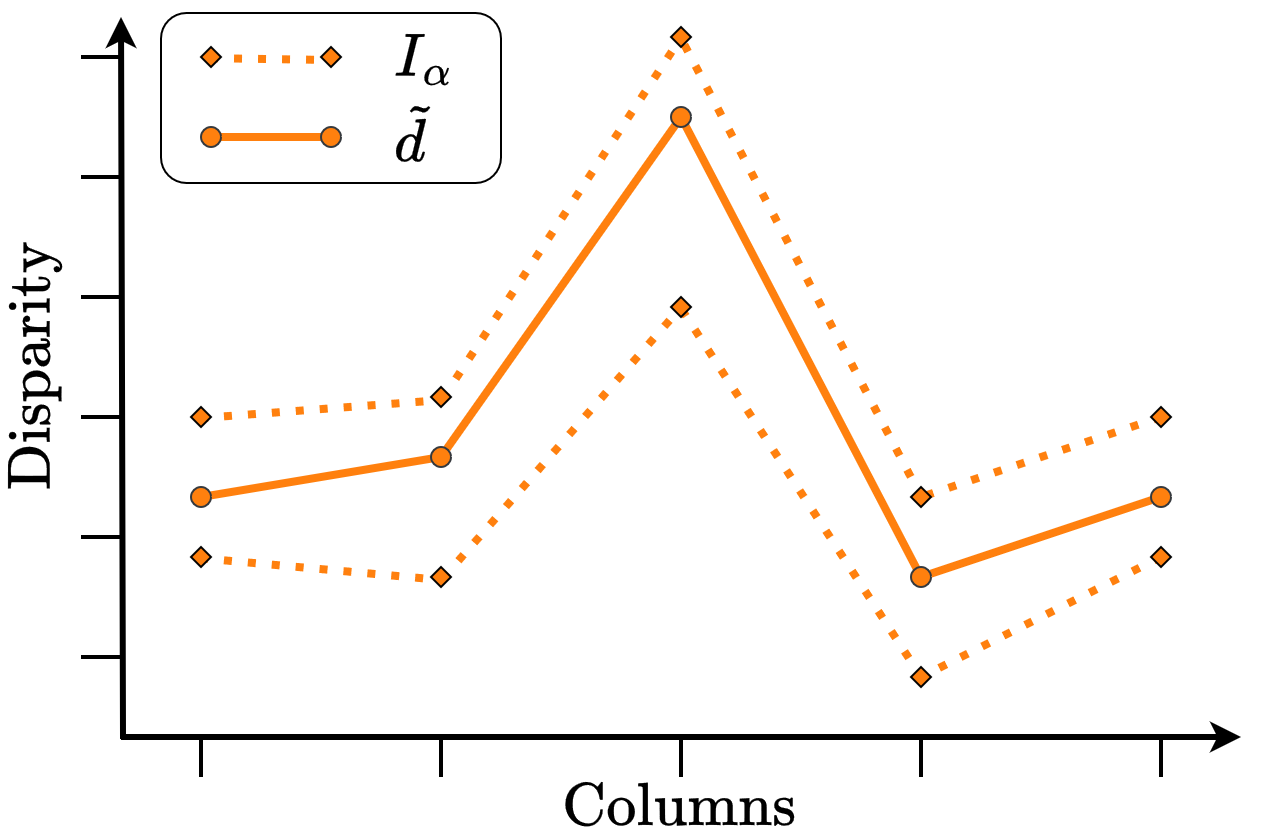
\includegraphics[width=\linewidth]{Images/Chap_5/Median_filtering_1.png}
        \caption{Without filtering}
        \label{fig:median_filtering_1}
    \end{subfigure}
    \hfill\begin{subfigure}[t]{0.32\linewidth}
        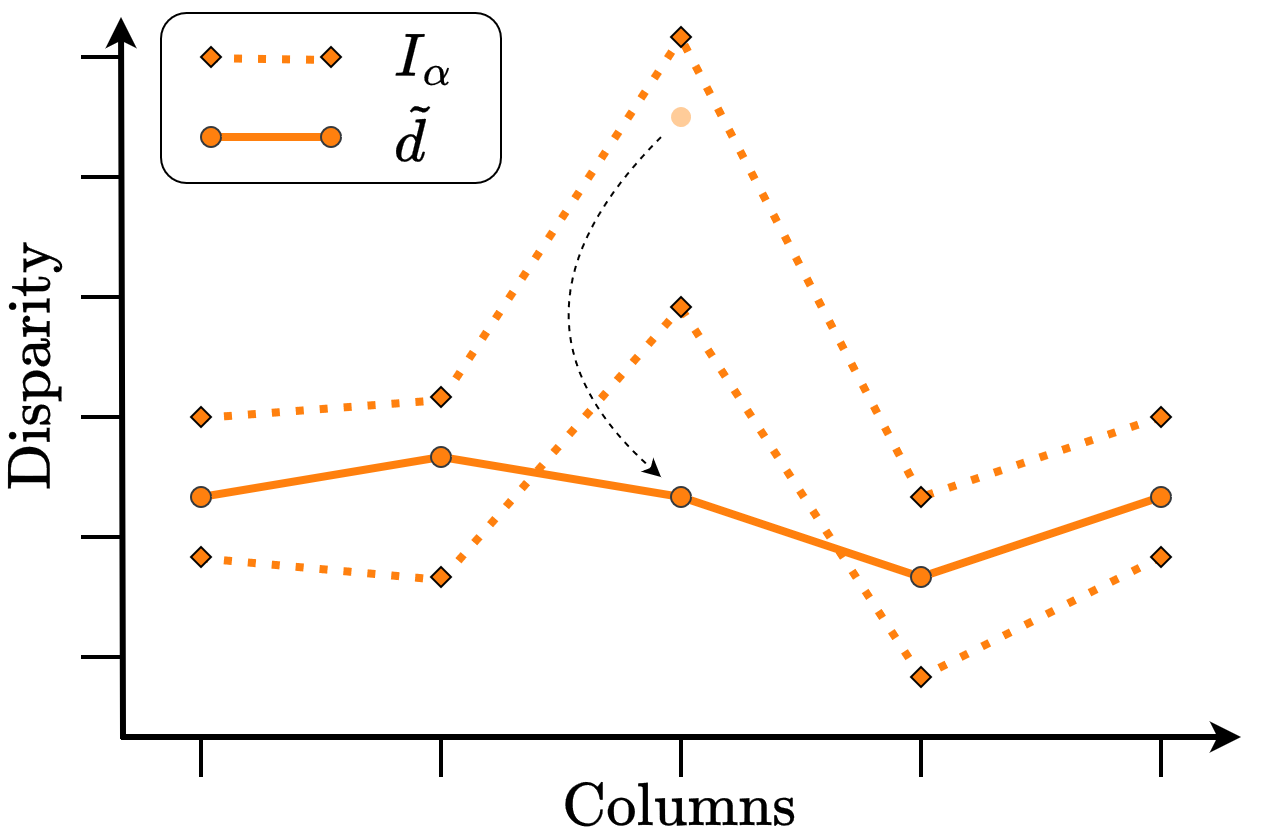
\includegraphics[width=1\linewidth]{Images/Chap_5/Median_filtering_2.png}
        \caption{Filtering only $\tilde{d}$}
        \label{fig:median_filtering_2}
    \end{subfigure}\hfill
    \begin{subfigure}[t]{0.32\linewidth}
        \centering
        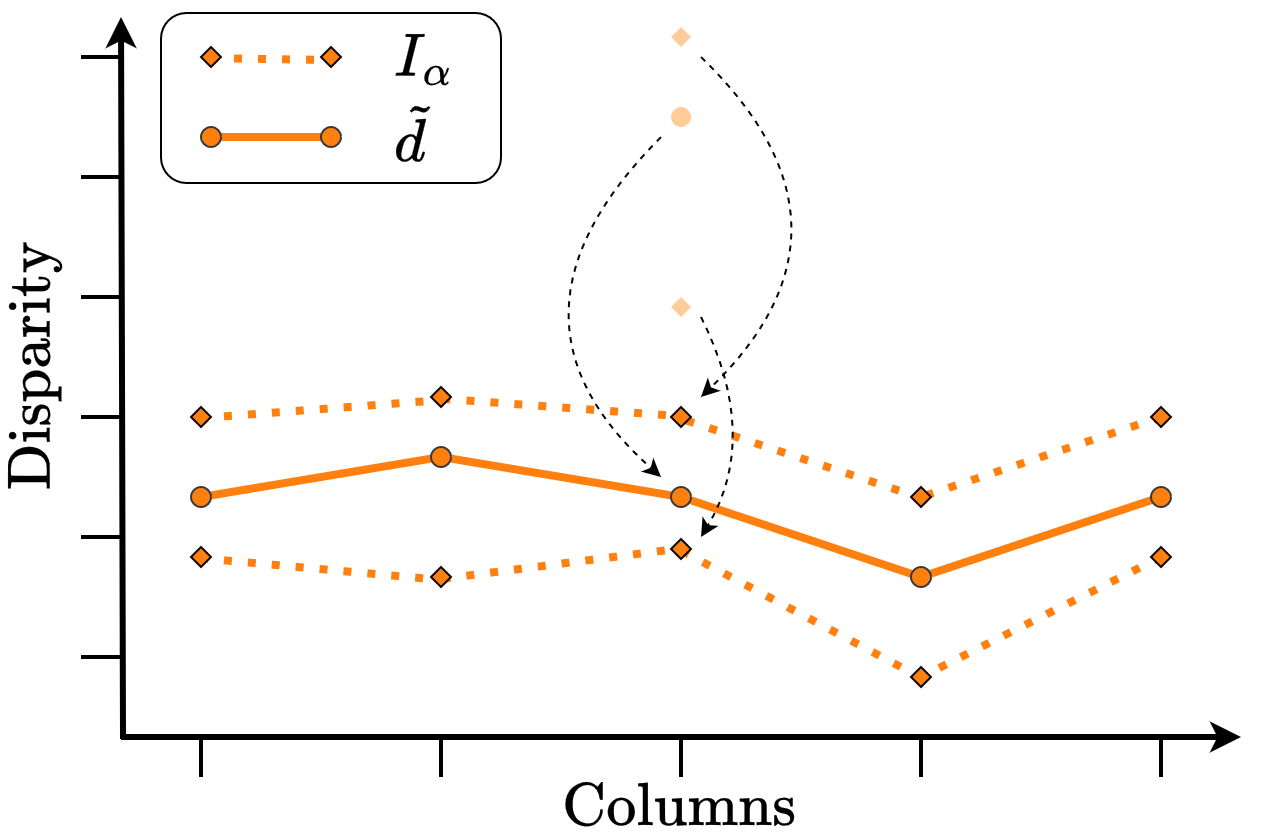
\includegraphics[width=\linewidth]{Images/Chap_5/Median_filtering_3.png}
        \caption{Filtering $\tilde{d}$ and $I_\alpha$}
        \label{fig:median_filtering_3}
    \end{subfigure}
    \caption{Effect of a median filter on the predicted disparity $\tilde{d}$ and confidence intervals $I_\alpha$. For the sake of the example, we only filter the middle point by looking at its neighbors. \Cref{fig:median_filtering_1} contains the unfiltered curves. \Cref{fig:median_filtering_2} contains unfiltered intervals, and filtered $\tilde{d}$. \Cref{fig:median_filtering_3} filtered intervals and filtered $\tilde{d}$.}
    \label{fig:median_filtering}
\end{figure}

Another processing applied to the disparity map is the sub-pixel refinement of its values, presented in \Cref{sec:stereo_matching} and \Cref{fig:sub-pixel_refinement}. The idea is to slightly modify the value of the disparity by interpolation of the cost curve, in order to obtain sub-integers disparity values. The modification cannot change a disparity more than a pixel away from its original value. If the predicted disparity $\tilde{d}$ equals one of the bounds of its confidence interval $I_\alpha$, the sub-pixel refinement step can shift the predicted disparity to a value slightly outside the confidence intervals. In this case, we simply extend the interval by one pixel. For instance, if $\tilde{d}=\underline{I}_\alpha$, then the new confidence interval $I_\alpha'$ equals:
\begin{align}\label{eq:subpixel_intervals}
    I_\alpha'=[\underline{I}_\alpha-1,~\overline{I}_\alpha]
\end{align}
This stretching is simple, and also presents the advantage of working with different\commanue{any} type of sub-pixel refinement (\ie V-fit, parabola \etc).

\subsection{Regularization of Intervals in Low Confidence Areas}\label{sec:regularization_of_intervals}
We saw that disparity intervals have\commanue{disparity interval estimation has?} the potential to perform well even when the predicted disparity is far away from the ground truth\commanue{A voir, si ce ne serait pas intéressant de donner une métrique du genre avec cette première version de méthode on atteint pas les 90\% on est plutôt à XX\% donc blabla super Roman est là pour trouver une solution}. This model however encounters some performance issues near depth discontinuities. This can be explained as follows: as the \acrshort{sgm} regularization attempts to impose continuity on disparities, it results in cost curves that do not favor the correct disparity in the region where the continuity hypothesis is not valid. Considering that cost curves are equivalent to experts' opinions in those areas can be over-optimistic, and the resulting intervals thus cannot be completely trusted. We will now present how we can adapt the model on those regions, in order to correct those flaws.

The first challenge to tackle is to determine if we are able to detect regions where discontinuities occur, in order to process intervals differently there\commanue{there differently plutôt ?}. Using the predicted disparity map might be a lead, but we saw in \Cref{fig:intervals_ambiguous_row_80,fig:intervals_ambiguous_row_180,fig:intervals_ambiguous_row_240,fig:intervals_ambiguous_row_290} that there is usually a shift between predicted disparity discontinuities and true disparity discontinuities. Instead, we can consider confidence measures\commanue{we could consider to use confidence measures?} computed alongside the disparity map, which are usually good candidates to detect discontinuities. In particular, we consider\commanue{choose car trop de consider tue le consider} the confidence from ambiguity measure $c_{Amb}$ presented in \cref{eq:confidence_from_ambiguity} from \Cref{chap:stereophotogrammetry}. Note that other confidence measures could be considered instead of the ambiguity, but this confidence measure has the advantage of performing well, being explainable (which is not always the case for learning-based measures) and being already implemented in the stereo pipeline we use. \Cref{fig:wrong_intervals_and_ambiguity} shows that pixels with wrong intervals $I_\alpha$ usually present a low confidence from ambiguity as well, meaning that we should be able to use this confidence measure to process confidence intervals differently.

\begin{figure}
    \centering
    \begin{subfigure}[t]{0.3\linewidth}
        \centering
        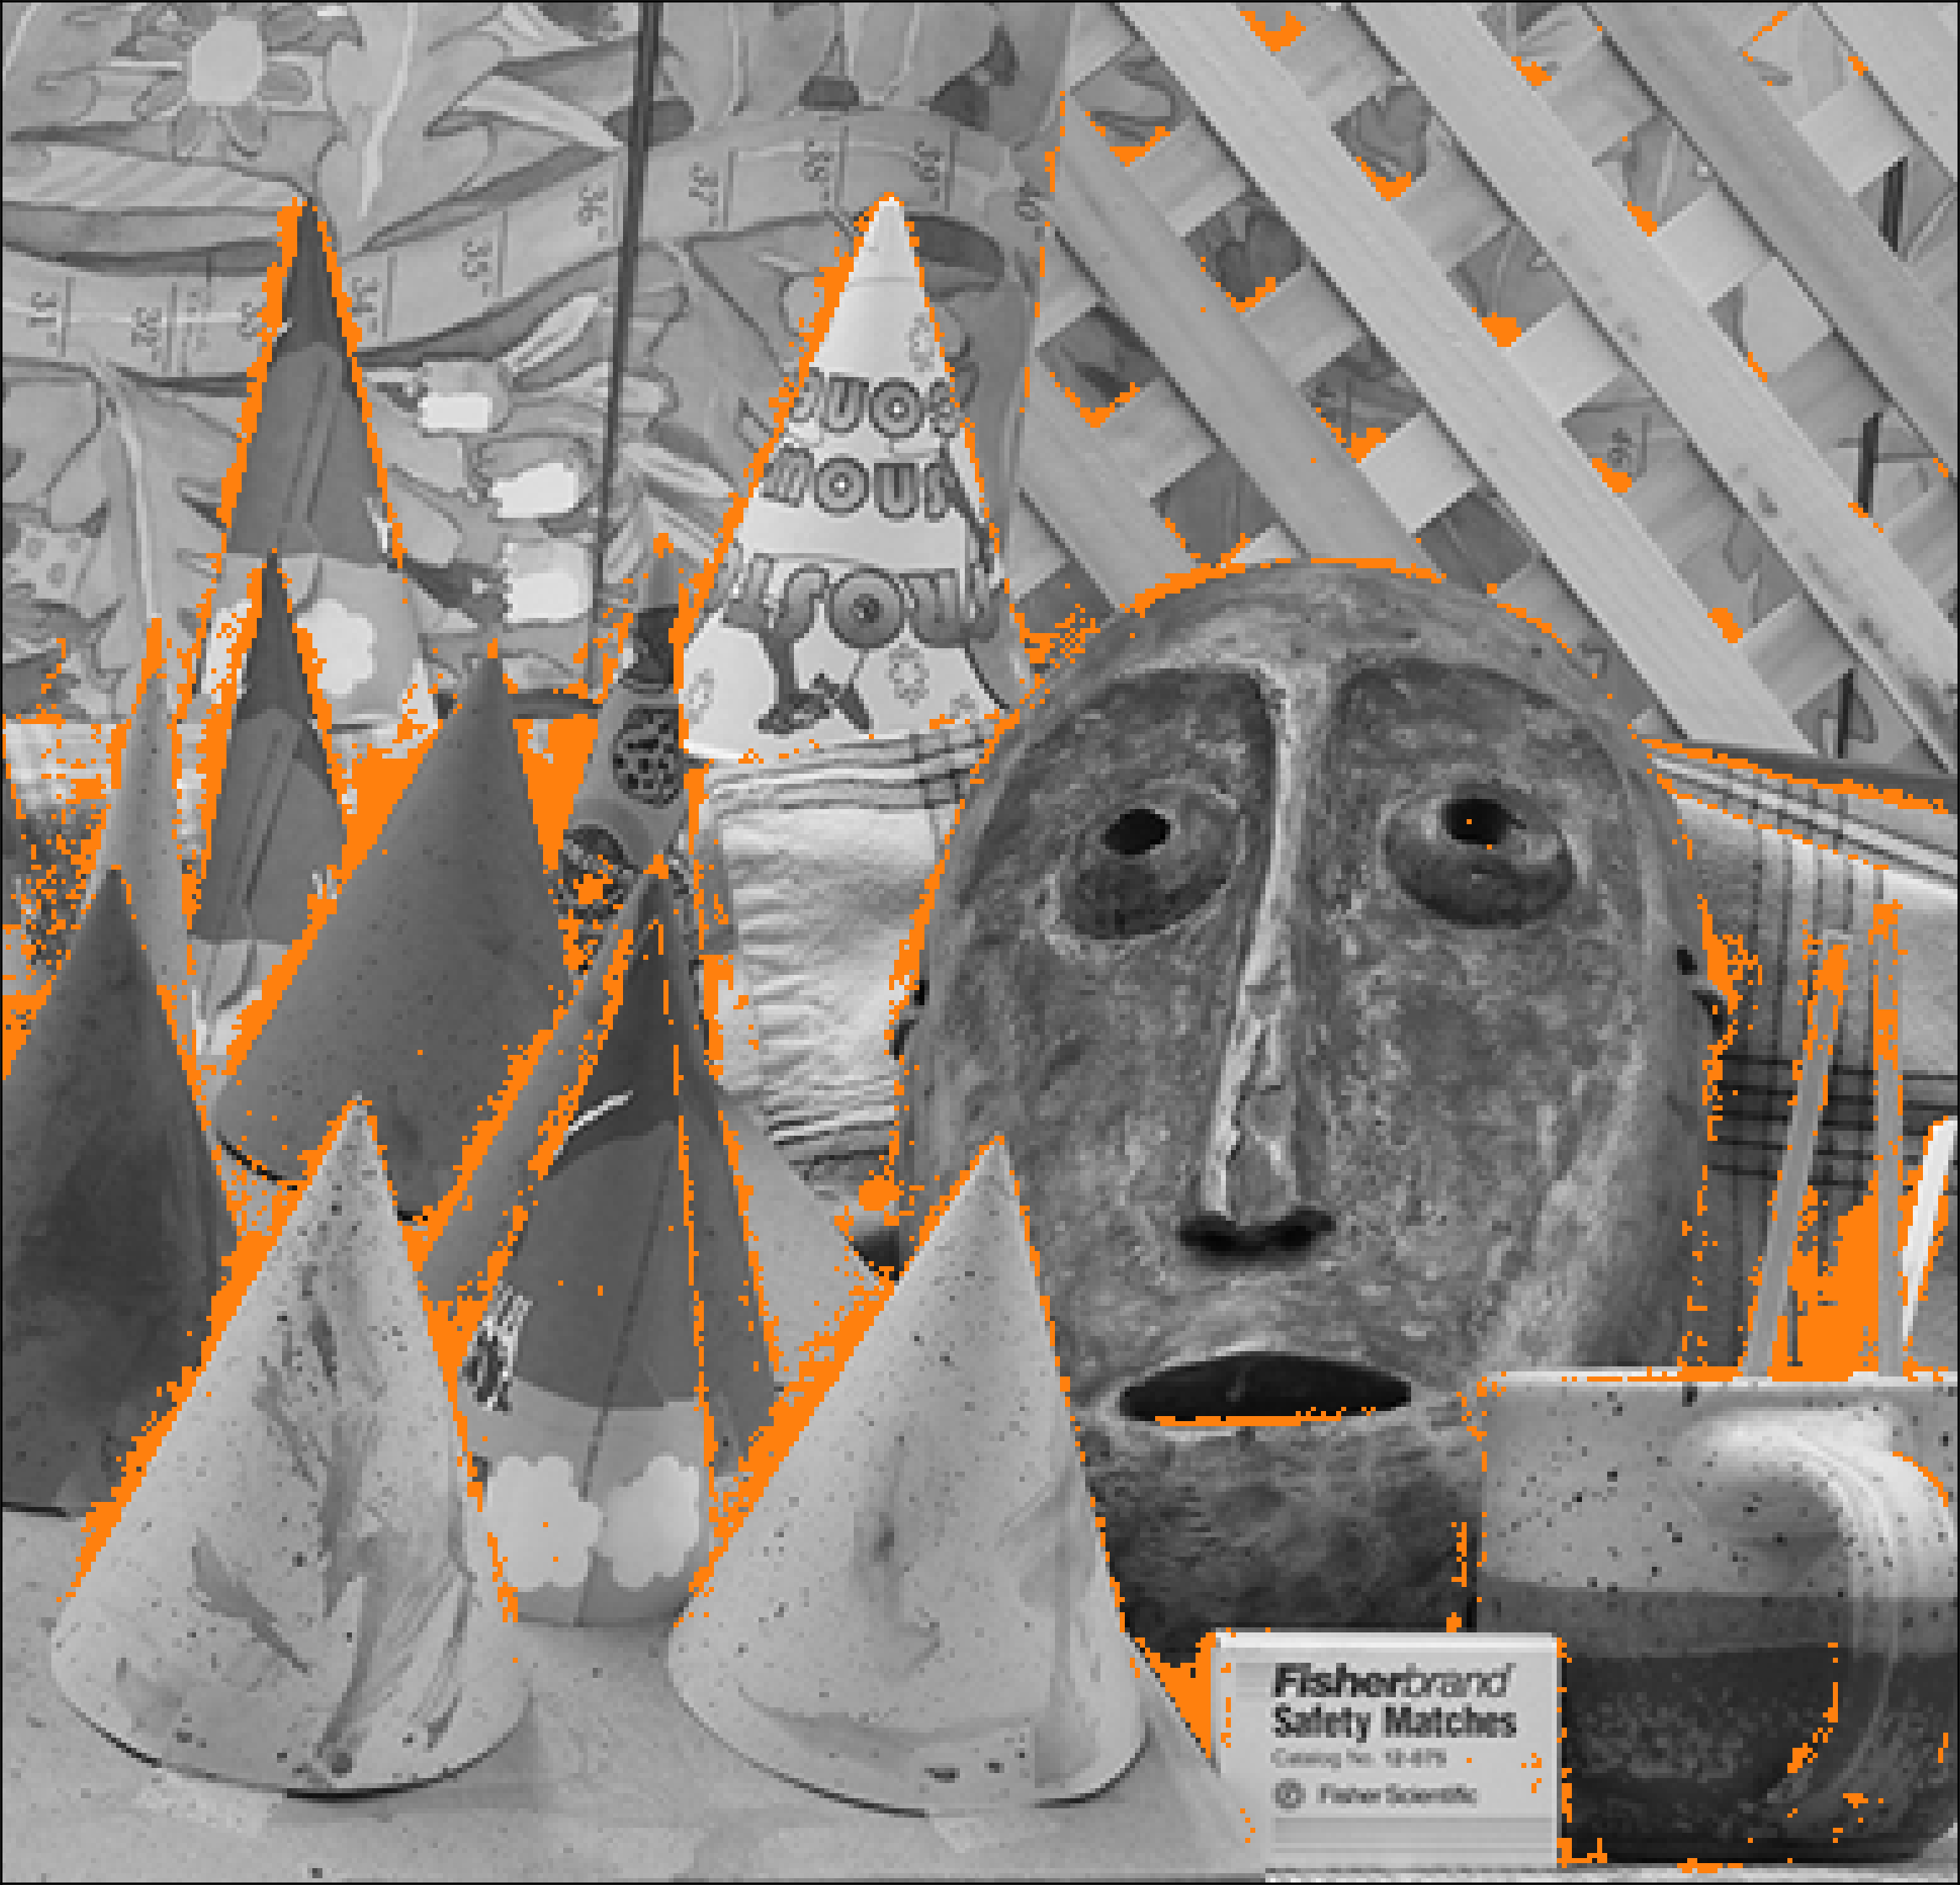
\includegraphics[width=\linewidth]{Images/Chap_5/wrong_intervals_no_reg.png}
        \caption{Left stereo image. Pixels where $d_{true}\not\in I_\alpha$ appear in orange.}
        \label{fig:wrong_intervals}
    \end{subfigure}\hfill
    \begin{subfigure}[t]{0.3\linewidth}
        \centering
        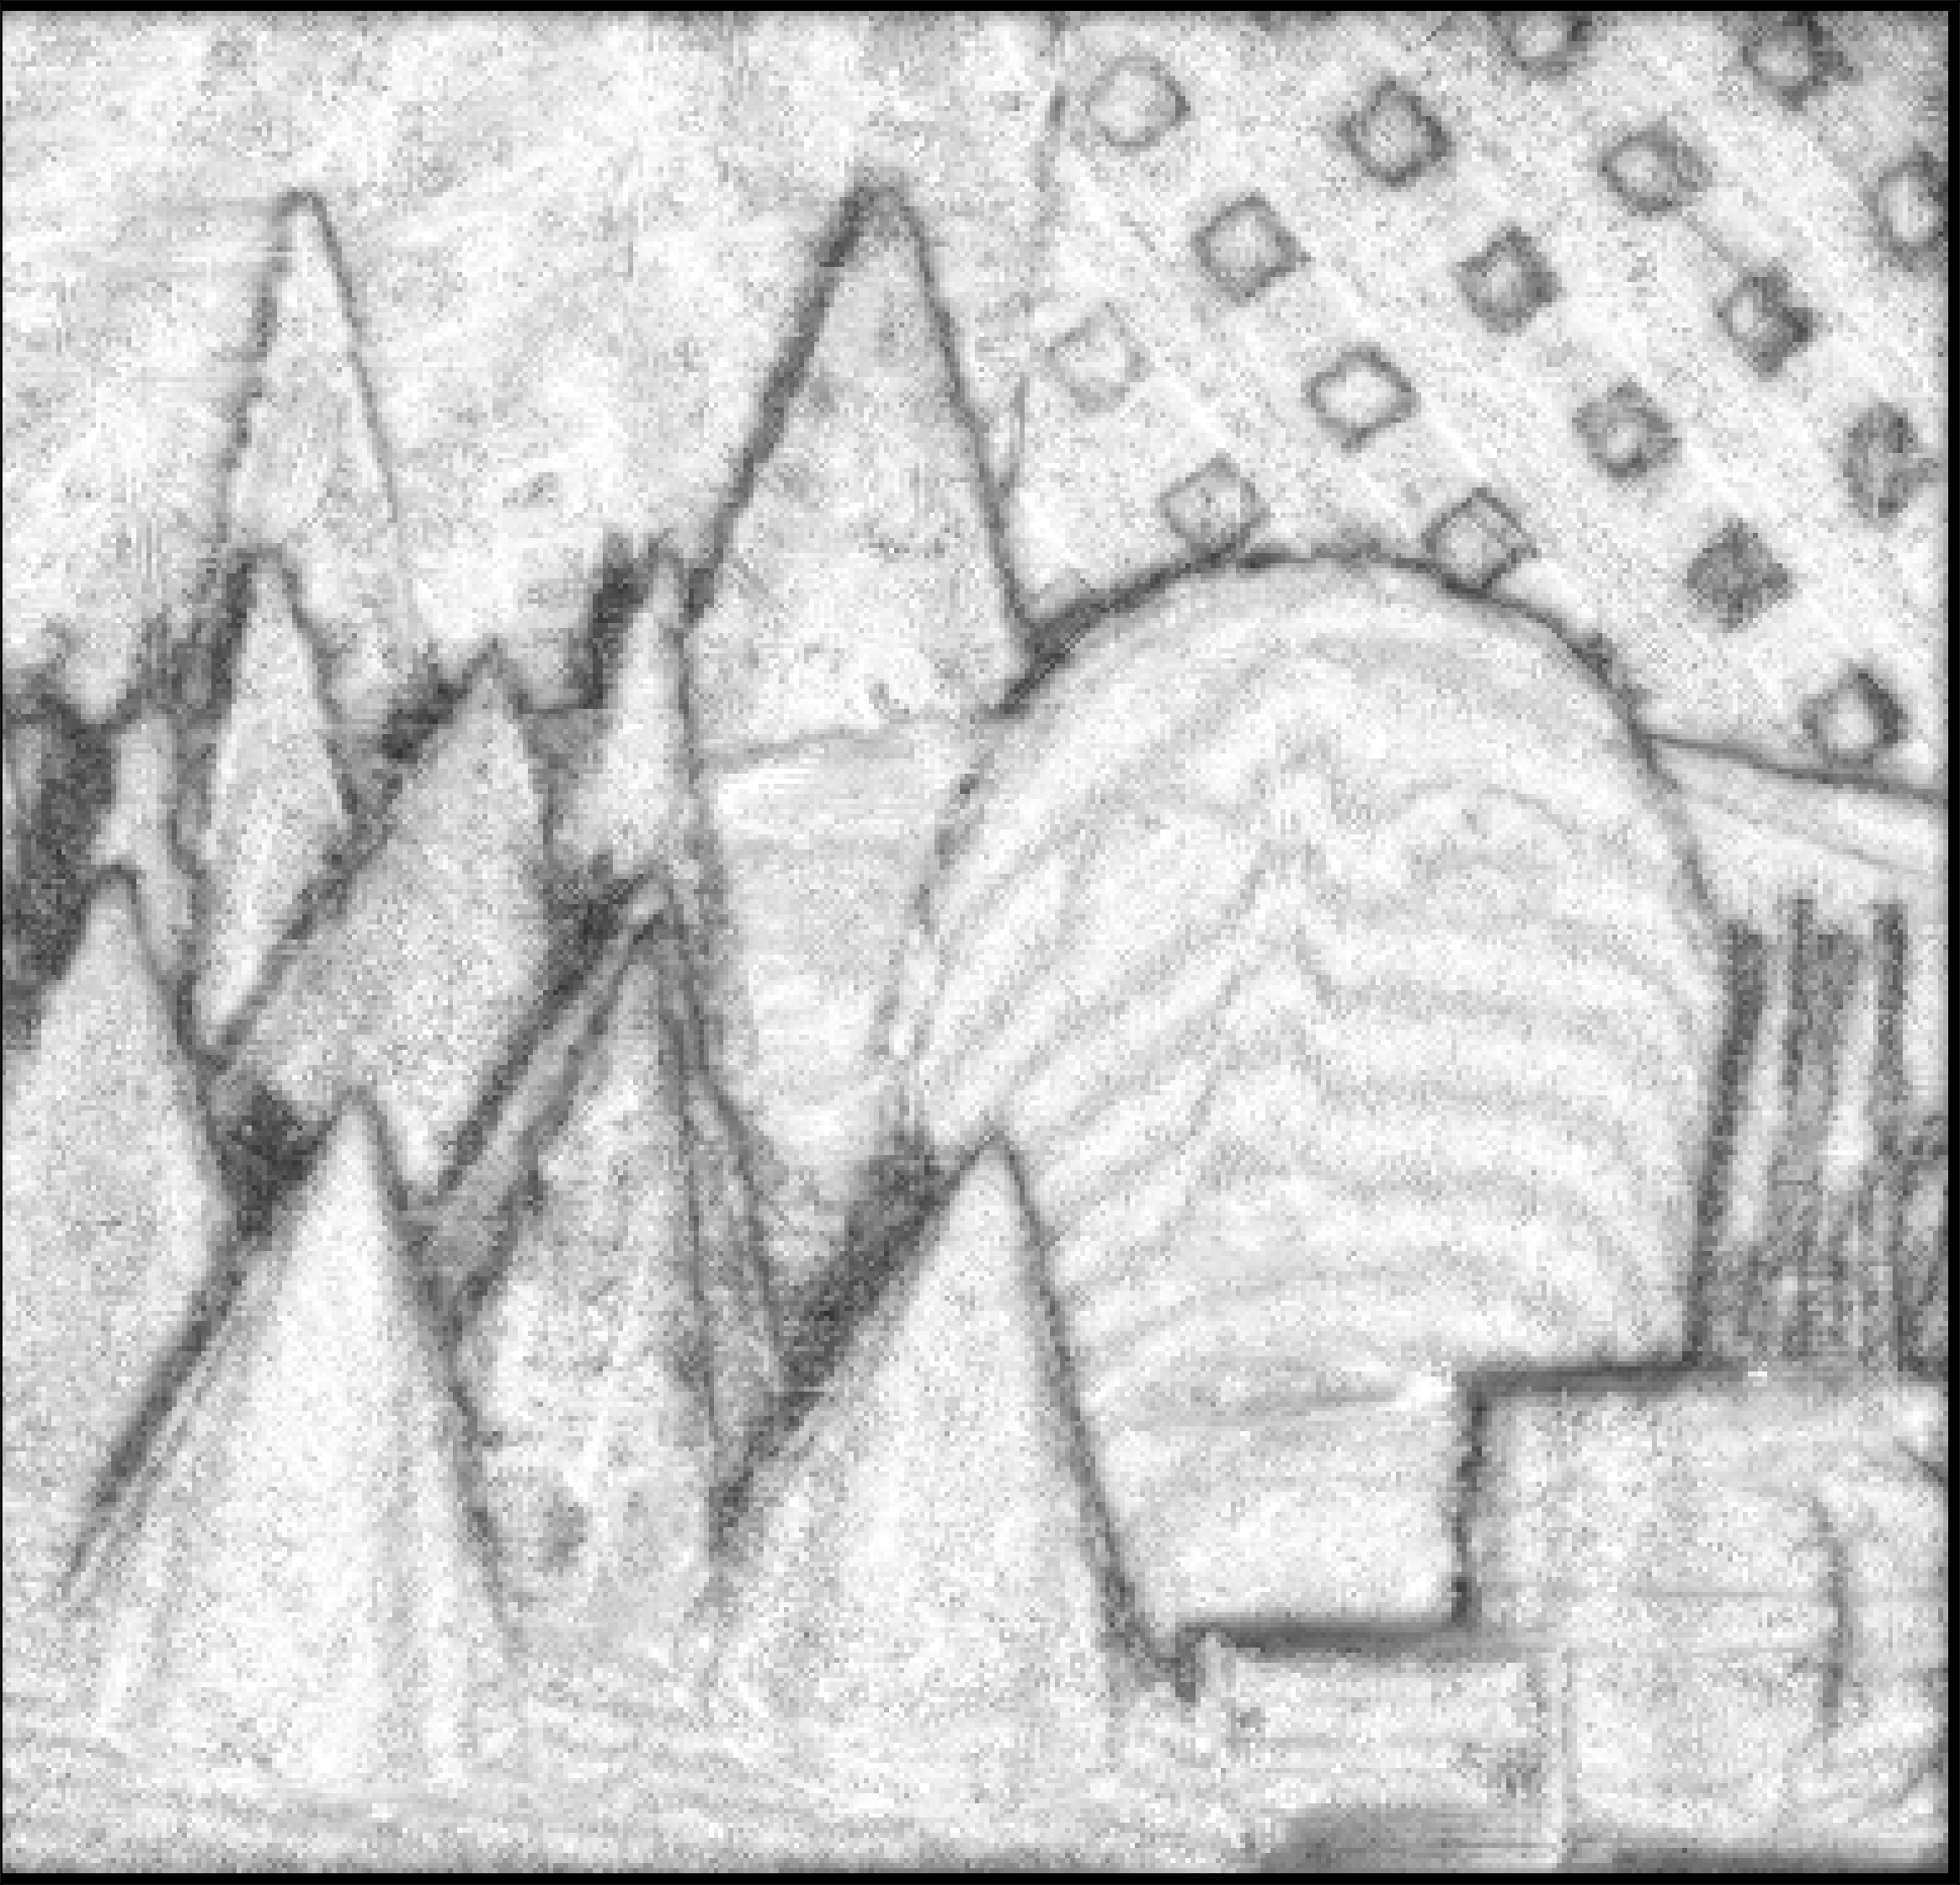
\includegraphics[width=\linewidth]{Images/Chap_5/ambiguity_cones.png}
        \caption{Confidence from ambiguity $c_{Amb}$. Dark pixels have a low confidence, bright pixels have a high confidence.}
        \label{fig:ambiguity_cones}
    \end{subfigure}\hfill
    \begin{subfigure}[t]{0.3\linewidth}
        \centering
        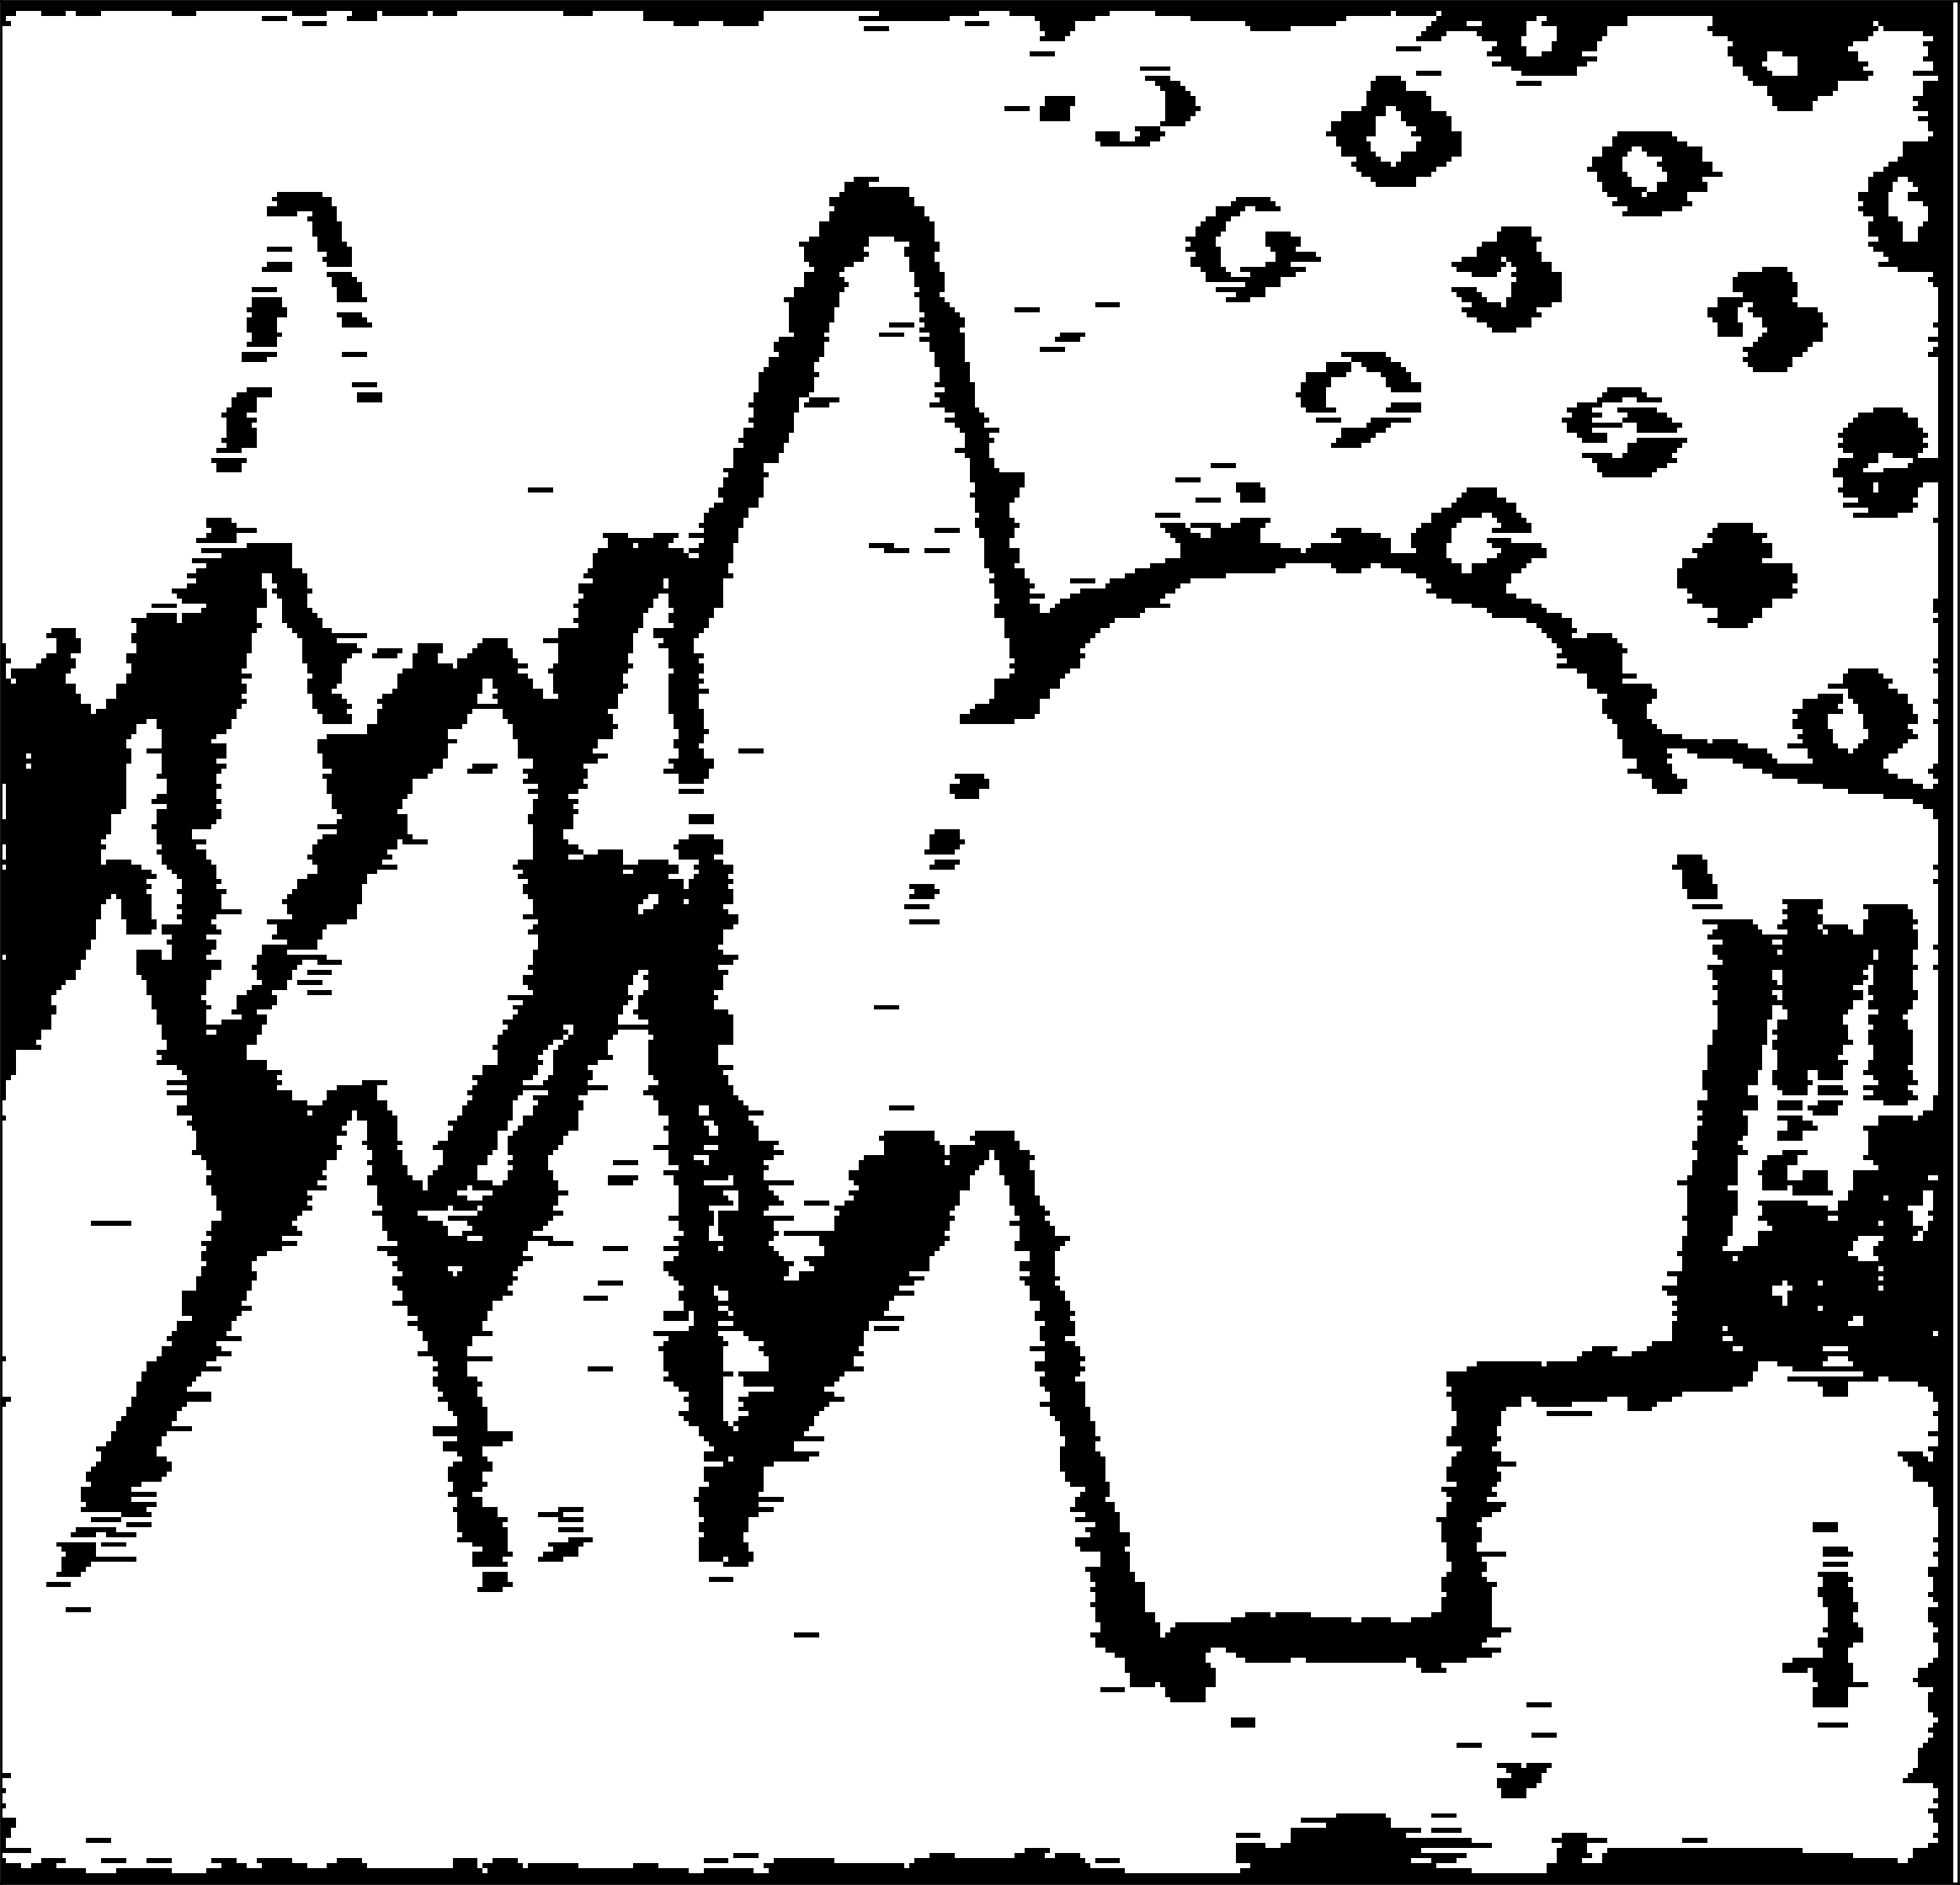
\includegraphics[width=\linewidth]{Images/Chap_5/ambiguity_mask_cones.png}
        \caption{Binary mask, low confidence areas are indicated by black pixels.}
        \label{fig:ambiguity_mask_cones}
    \end{subfigure}
    \caption{Position of wrong intervals in the left image, the corresponding confidence map and the low confidence area mask obtained using \cref{eq:low_confidence_area}}
    \label{fig:wrong_intervals_and_ambiguity}
\end{figure}

\begin{remark}\commanue{j'ai rien contre la remarque elle-même mais alors elles arrivent jamais au bout moment par rapport à ce qui est développé dans le corps principal du texte. Peut-être fait une paragarphe dédié au debut sur l'image que tu considères. Il me semble que tu as une phrase ou deux sur les cônes et ensuite tu places cette info direct dans le texte sans faire un encart. J'ai parfois l'impression que l'encart remark te permet de dire qqch que tu as oublié de mentionner avant, plutôt que quelque chose d'annexe.}
    In all of our experiments, we do not consider pixels where the whole range of considered disparities cannot be explored. For instance, in the case of the Cones image from the Middlebury dataset, the range of considered disparities is $[-60,0]$ which means that we do not the consider the 60 left-most pixels of the image.
    
    We proceed this way because for the most part, the true disparity of those pixels do not exist\commanue{peut-être dire que tu le sais car tu as la vérité terrain qui le confirme et par conséquent tu sais que le point homologue qui serait nécessaire est en fait absent de l'image de droite}. Additionally, the \acrshort{sgm} regularization will also predict a false disparity (as the true disparity does not exist) and base the regularization of the neighboring disparities based on this false prediction. This greatly compromises the disparity prediction, the quality of intervals \etc Those pixels are thus masked.
\end{remark}

The method developed for detecting low confidence areas is to apply a simple threshold $\tau_{Amb}$ on the confidence from ambiguity $c_{amb}$. However, $c_{Amb}$ is computed pixel-wise, which can lead to high-frequency spatial variations of the confidence. To smooth the ambiguity curve, a minitive kernel of size $(1, ~2\times k_{Amb}+1)$ is applied. A pixel $(\rowcol)$ is thus considered to be in a low confidence area if it verifies:
\begin{align}\label{eq:low_confidence_area}
    \min_{-k_{Amb}~\leqslant~ k~\leqslant ~k_{Amb}}c_{Amb}(\rowcol+k)\leqslant \tau_{Amb}
\end{align}
We used $k_{Amb}=2$ and $\tau_{Amb}=0.6$ in our experiments. For simplicity, we will refer to $\min c_{Amb}$ instead of $min_{-k_{Amb}~\leqslant~ k~\leqslant ~k_{Amb}}c_{Amb}$ in the following. Additional investigations on those parameters are presented in annex \todoroman{Mettre les ablation study en annexe}. \Cref{fig:ambiguity_kernel} illustrates the impact of smoothing the confidence from ambiguity, and displays the threshold used to detect low confidence areas. We can see around columns $185$ and $320$ that the kernel smooths isolated confidence values that would not be detected by the threshold otherwise. \Cref{fig:ambiguity_mask_cones} presents the position of pixels in low confidence areas over the whole left image. As a quick indicator of this method performances, $83\%$ of intervals that do not contain the ground truth (orange pixels in \Cref{fig:wrong_intervals}) are also contained in low confidence areas. Once again, it is possible to use any other confidence measure to detect areas where intervals perform badly. The choice of this method in particular lies on its good performances while remaining simple in comprehension and implementation.

\begin{figure}
    \centering
    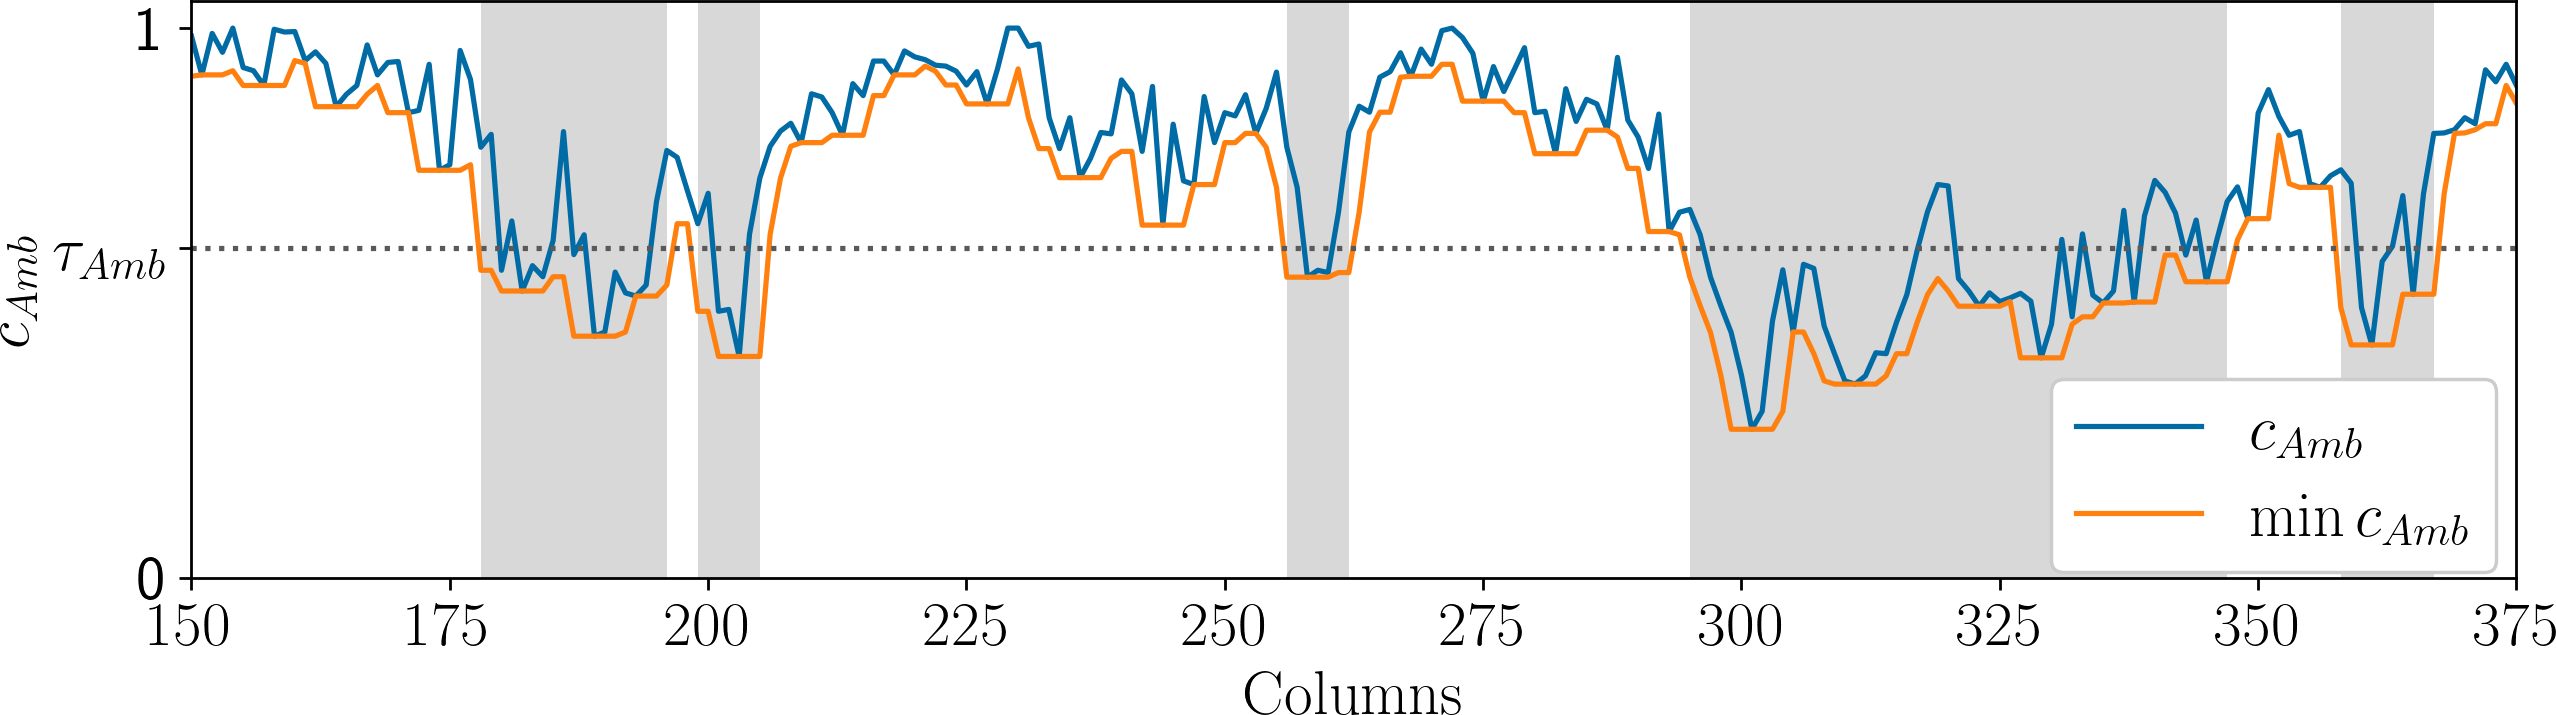
\includegraphics[width=\linewidth]{Images/Chap_5/ambiguity_kernel_row_110.png}
    \caption{Confidence from ambiguity $c_{Amb}$, smoothed confidence $\min c_{Amb}$ from \eqref{eq:low_confidence_area} for row $110$ of the Middlebury Cones image. Low confidence areas, where $\min c_{Amb}$ is less than $\tau_{Amb}$ are highlighted in gray.}
    \label{fig:ambiguity_kernel}
\end{figure}

Having computed regions of low confidence, we can now process the intervals differently in those areas. The main idea here is that information contained in low confidence cost curves should be handled with care. The hypothesis that a cost curve can be interpreted as an expert stating his opinion on which disparities are most probable is questionable in those areas. We also cannot infer the confidence intervals from intervals in neighboring high confidence areas as there is no guarantee the disparities are the same as their high confident neighbors. We instead chose to proceed in two steps. First, we compute a neighboring set of intervals for each low confidence pixel. Then, we use the information from this set to determine a new disparity interval by consensus. We modify the value of the considered pixel with that of this\commanue{c'est bizarre comme formulation} consensual interval.

We first detail how the set of neighboring pixels is determined. Let $(\rowcol)$ be a low confidence pixel. We define a segment $S(\rowcol)$ as the set containing $(\rowcol)$ and all adjacent low confidence pixels from the same row. An example of $S(\rowcol)$ is presented in \Cref{fig:low_confidence_segments} as an orange rectangle. Two segments $S(\rowcol)$ and $S(row+1, ~col')$ are considered adjacent if two of their pixels are directly on top of one another. The low confidence neighboring $\N(row,~col)$ is defined as the set of low confidence pixels in segment $S(\rowcol)$ or in adjacent segments within $n$ rows. In practice, we use $n=3$. The formal definition of $S(\rowcol)$ and $\N(row,~col)$ introduced next can be a bit heavy on notations, so we refer to \Cref{fig:low_confidence_segments} for a graphical example of what they represent. $S(\rowcol)$ is formally defined as:
\begin{align}
    S(\rowcol) = \{~ (row,~col') \text{ \st }~\forall c\in\opi col, col'\cli,~\min c_{Amb}(row, ~c+k)\leqslant \tau_{Amb}~\}
\end{align}
where $\opi col, col'\cli$ supposes that $col\leqslant col'$, and is replaced by $\opi col', col\cli$ if not. The formal definition of $\N(row,~col)$ is then:
\begin{align}
    \N(row,~col) = \{ p\in &\bigcup_{-n\leqslant k\leqslant n}S(row+k, ~col_k)\nonumber\\
    &\st~S(row + (k+1), ~col_{k+1})\text{ is adjacent to }S(row+k, ~col_{k})\}
\end{align}
with $col_0=col$, and $n$ the number of consecutive rows considered.\commanue{dans mes souvenirs c'était plus clair dans CVPR et le schéma aussi}

\begin{figure}
    \centering
    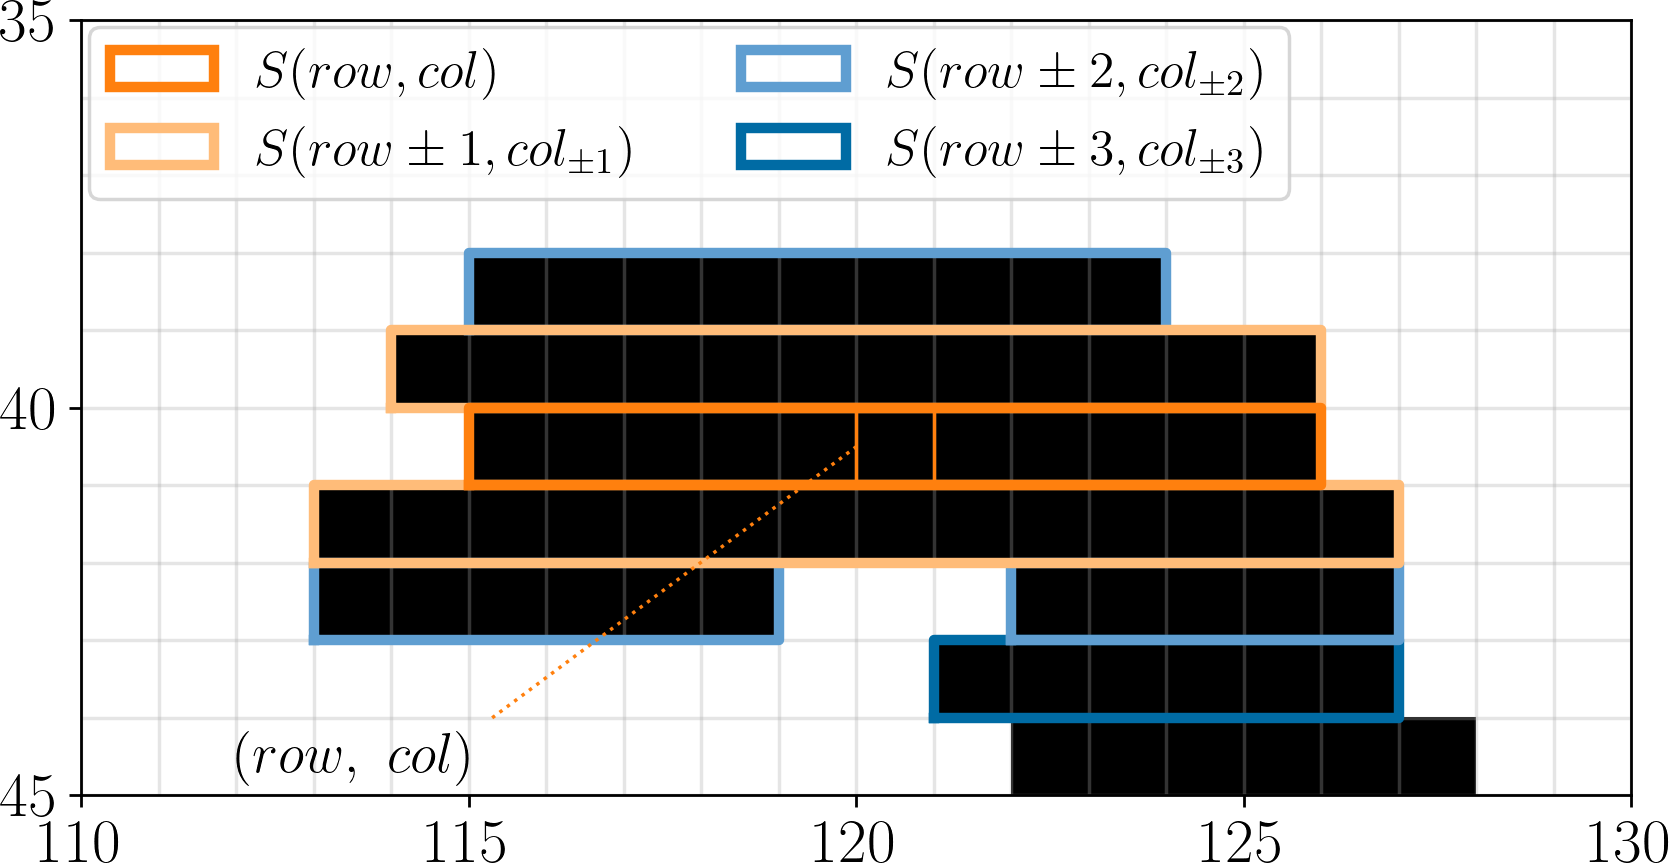
\includegraphics[width=0.7\linewidth]{Images/Chap_5/low_confidence_segments.png}
    \caption{Segment $S(row, ~ col)$ and its adjacent segments over $3$ rows above and below. The image is an extract of the binary mask from \Cref{fig:ambiguity_mask_cones}, where low confidence pixels appear in black and high confidence pixels appear in white.}
    \label{fig:low_confidence_segments}
\end{figure}\todoroman{Split la figure pour que ça corresponde à chaque étape de la description (avec un seul segemnt, puis les lignes +-1 etc}

The value of the regularized interval $I^{reg}_\alpha$ of $(\rowcol)$ is obtained by consensus between the confidence intervals of $\N(\rowcol)$. Its upper and lower bounds are respectively the $q$\ith quantile of upper bounds of $\N(\rowcol)$ and the $(1-q)$\ith quantile of lower bounds of $\N(\rowcol)$:
\begin{align}
    I^{reg}_\alpha=[\mathcal{Q}_\N(1-q), ~\mathcal{Q}_\N(q)]
\end{align}
where $\mathcal{Q}_\N(q)$ refers to the $q$\ith quantile of $\N(\rowcol)$. In practice, we use $q=90\%$. This way, the lower bound of $I^{reg}_\alpha$ is lower than that of $90\%$ of intervals in $\N(\rowcol)$, and its upper bound is larger than that of $90\%$ of intervals in $\N(\rowcol)$. 

\begin{remark}
    It does not necessarily mean that $I^{reg}_\alpha$ includes $90\%$ of intervals of $\N(\rowcol)$. Indeed, there can be intervals whose lower bound is greater than the $(1-q)$\ith lower bounds quantile while also being greater than the $q$\ith upper bounds quantile. The intervals will then overlap while not being included in one another.
\end{remark}

We can notice that it is possible, although unlikely, that the $q$\ith quantile of the upper bounds of $\N(\rowcol)$ is lesser than the predicted disparity $\tilde{d}(\rowcol)$ (or similarly, the $(1-q)$\ith quantile of lower bounds can be greater than $\tilde{d}(\rowcol)$). In that case, in order to insure the coherence of the predicted disparity with the confidence intervals, the bounds of the intervals are extended until they include $\tilde{d}$.

With the way $\N(\rowcol)$ is defined, every pixel of $S(\rowcol)$ will have the same value for their regularized interval $I^{reg}_\alpha$. This can be observed in \Cref{fig:intervals_ambiguous_row_80_2,fig:intervals_ambiguous_row_180_2,fig:intervals_ambiguous_row_240_2,fig:intervals_ambiguous_row_290_2}\commanue{je suis pas fan d'avoir les figures 4 pages avant}, where positions of low confidence pixels that are regularized are indicated with gray areas. As we regularize every intervals in low confidence areas, we will refer to them simply as $I_\alpha$ in the following.

In theory, it is possible to perform the regularization of intervals before the filtering and refinement steps, but we chose to always regularize the intervals after those steps\commanue{ok ça explique l'ordre des paragraphe}. This prevent outliers removed by the filtering step to influence values of regularized intervals. \Cref{fig:intervals_ambiguous_row_80,fig:intervals_ambiguous_row_180,fig:intervals_ambiguous_row_240,fig:intervals_ambiguous_row_290} allow to visualize the impact of the regularization of intervals after the filtering and refinement steps. We can see that the regularization allows to create correct confidence intervals in \Cref{fig:intervals_ambiguous_row_80_2} near column $215$. In \Cref{fig:intervals_ambiguous_row_180}, columns $70$ and $175$ also create correct intervals, in regions where the predicted disparity $\tilde{d}$ is far away from the ground truth. Because\commanue{alors je ne suis pas sure de comprendre comment la justification explique le reste de la phrase} intervals are constant in low confidence areas (gray areas in the figure), we can say that the intervals are (almost) as small as possible so as to both contain $\tilde{d}$ and the true disparity $d_{true}$. Column $175$ of \Cref{fig:intervals_ambiguous_row_180} also shows that filtering and regularization methods are able to discard outliers: bounds of non-regularized intervals reach values between $-60$ and $0$ near column $175$, while the bounds of regularized intervals stay between $-42$ and $-15$. However, this method is not perfect, as it sometimes over estimates the size of intervals as in \Cref{fig:intervals_ambiguous_row_290_2} near column $110$, or do not predict correct intervals at all, as observed around column $450$.

\begin{figure}
    \centering
    \begin{subfigure}[t]{0.49\linewidth}
        \centering
        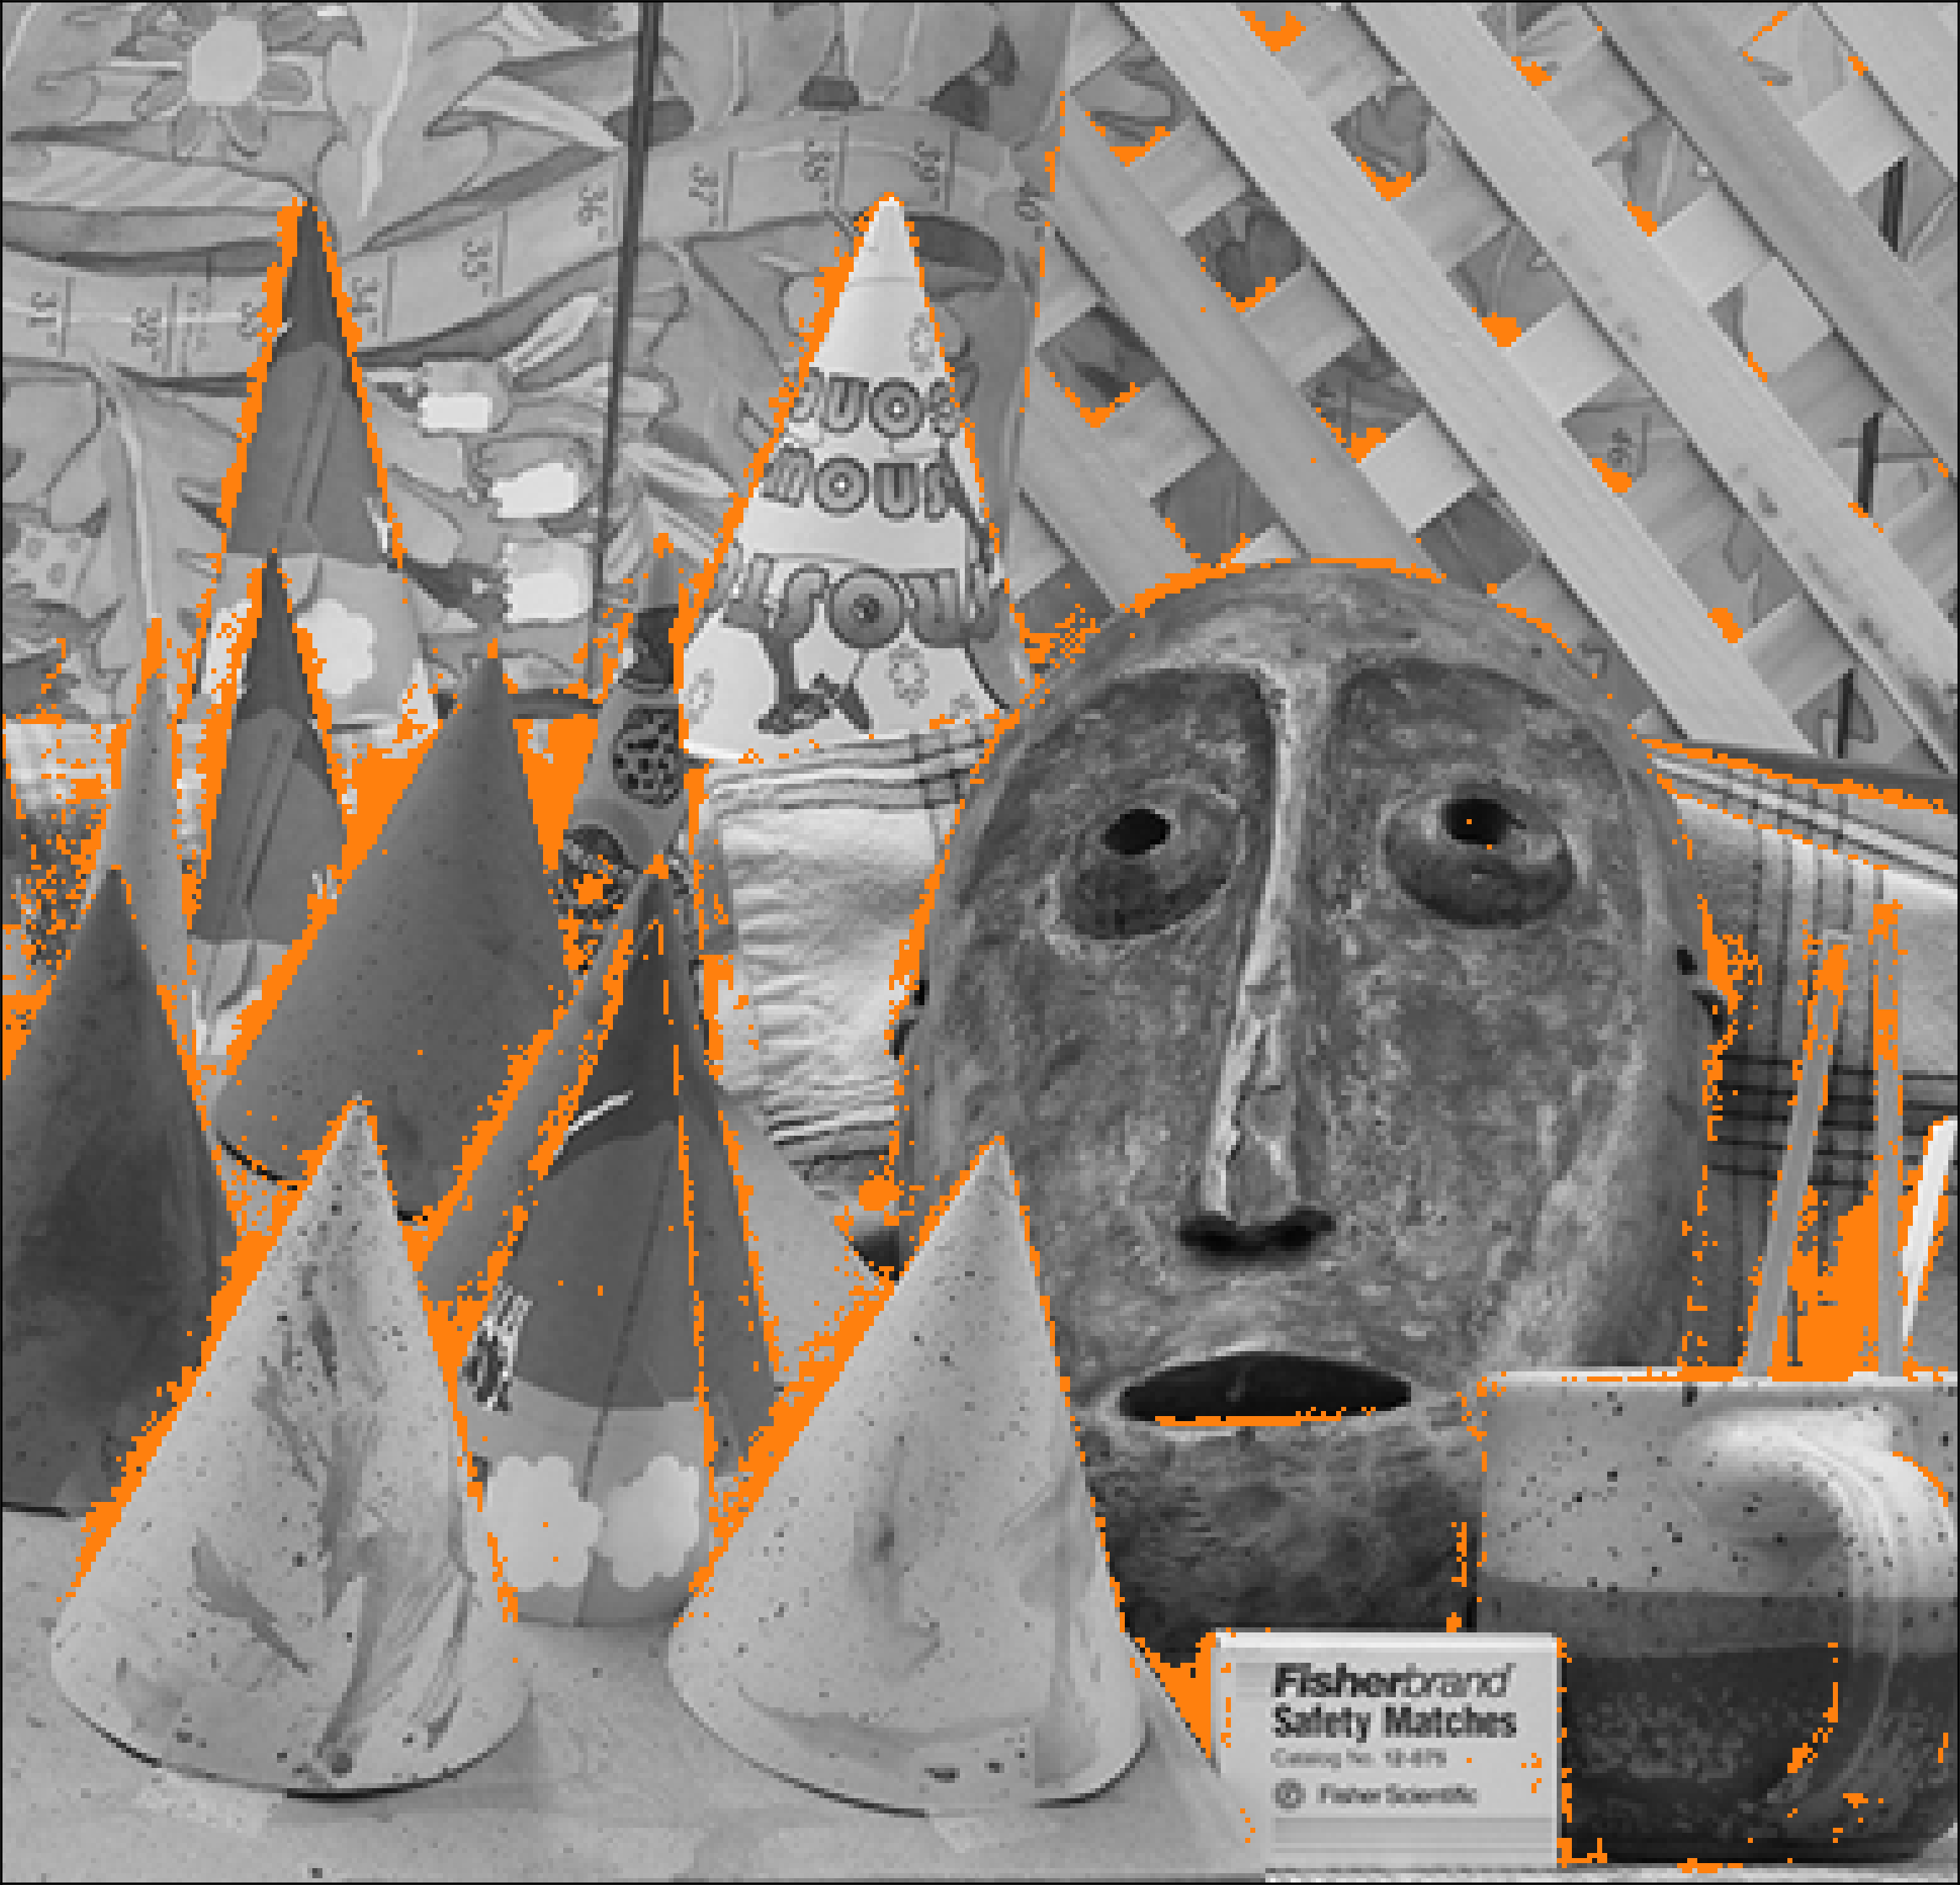
\includegraphics[width=\linewidth]{Images/Chap_5/comparison_wrong_intervals_no_reg.png}
        \caption{Without regularization, filtering and refinement}
        \label{fig:comparison_wrong_intervals_no_reg}
    \end{subfigure}
    \hfill\begin{subfigure}[t]{0.49\linewidth}
        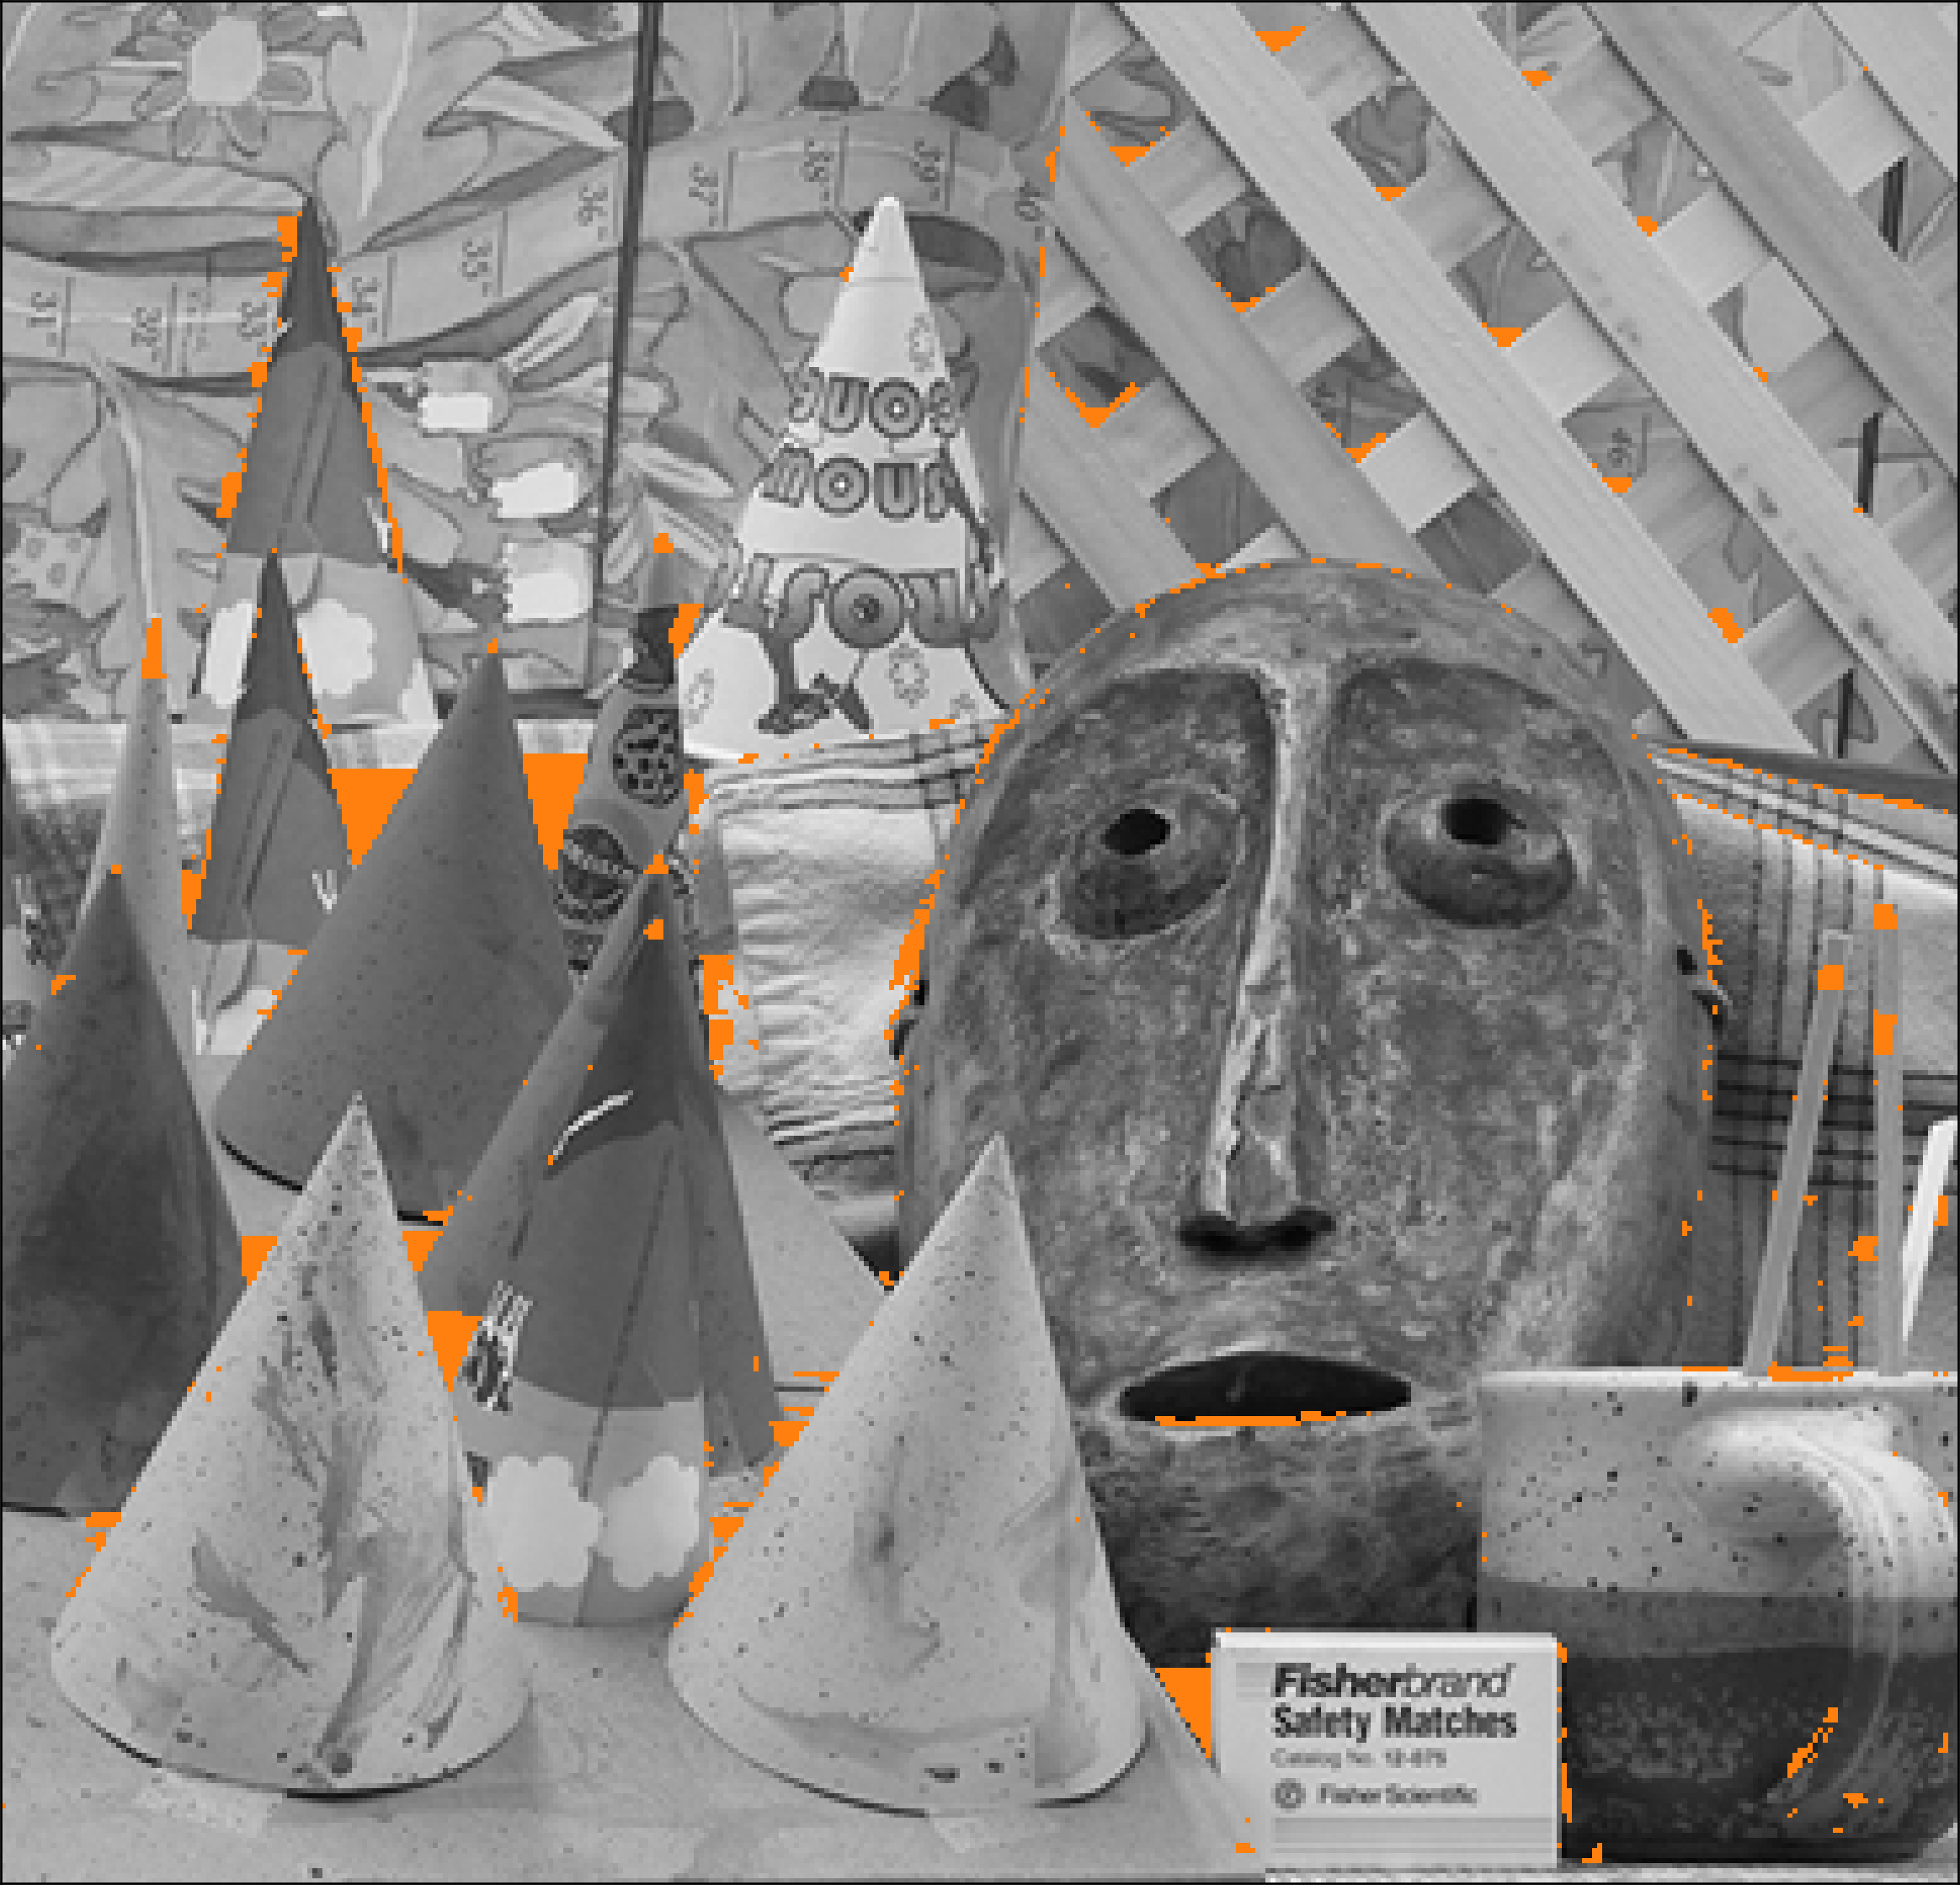
\includegraphics[width=1\linewidth]{Images/Chap_5/comparison_wrong_intervals_reg.png}
        \caption{With regularization, filtering and refinement}
        \label{fig:comparison_wrong_intervals_reg}
    \end{subfigure}
    \caption{Left image from Middlebury cones. Confidence intervals that do not contain the ground truth appear in orange.}
    \label{fig:comparison_wrong_intervals}
\end{figure}

\Cref{fig:comparison_wrong_intervals} allows to visualize the position of wrong intervals in the left stereo image. We can see clear improvements between the method with and without regularization, especially in the bottom right corner of images near the sticks inside the cup, or in general near cones borders. Quantitatively, wrong intervals represent around $5\%$ of pixels without regularization, and $1.6\%$ with regularization. Those numbers are presented for information purposes only, as further scores will be computed on different scenes, allowing for more in-depth analysis\commanue{peut-être que ça vaut le coup de mettre les réultats sur pandora ici. Là tu es parti pour mettre toute la théorie et ensuite les évaluations.}.

This concludes the method for computing confidence disparity intervals in the dense stereo matching part of the photogrammetry pipeline. We will see in the following how those intervals can be propagated into confidence intervals for the \acrshort{dsm}s.


\section{Evaluation of Disparity Intervals}
\subsection{Metrics for Evaluating the Precision and Size}\label{sec:metrics_disparity}
In order to evaluate the performances of the disparity confidence intervals, we will now introduce some metrics. The objective of this section is to propose a range of tools able to quantify the trade-off between accuracy and size of intervals. For all metrics, we do not consider pixels for which the ground truth does not exist, or pixels for which the predicted disparity $\tilde{d}$ has been removed by a cross-checking test (\cref{eq:cross-checking})\commanue{pixels without ground truth or pixels discarded by the cross-checking test, trop de relatives tuent la relative}. Also, many metrics are defined using the $\median$ of a set, instead of the mean, in order to be less sensitive to outliers\commanue{je ne sais pas si je mettrais la remarque là ou si j'attendrais la première définition pour dire que tu as décidé d'utiliser la médiane car blabla}. 

The first\commanue{pour des questions de lisibilité, je mettrai des sous-sous-section histoire d'avoir le titre de la métrique qui apparaît bien.} and most obvious metric is the proportion of correct intervals\commanue{comme je lis au fil de l'eau, je ne suis pas sure de ma remarque donc je ne sais pas si tu as explicitement défini ce qu'était un intervalle correct, genre i.e. intervals containing the true disparity}, which we call accuracy $acc$:
\begin{align}
    acc = \dfrac{\#\{I_\alpha ~|~ \st ~d_{true}\in I_\alpha\}}{\#\{I_\alpha\}}
\end{align}
We want to maximize the accuracy, but fixed ourselves a minimal objective of $90\%$ accuracy for our method.

It is also interesting to measure the magnitude of the error. We thus introduce another metric called residual error $\varepsilon$, computed for intervals that do not contain the ground truth and defined as:
\begin{align}
    \varepsilon=\median \left( \dfrac{\min(|d_{true}-\overline{I}_\alpha|, |d_{true}-\underline{I}_\alpha|)}{d_{max}-d_{min}}\right)\label{eq:residual_error}
\end{align}
where $[d_{min}, ~d_{max}]$ is the considered disparity range, which allows to compare the different images\commanue{Pour éviter les poupées russes de relatives, je ferais une phrase séparée: Normalization by the disparuty range gives us a metric that is independent of disparity range, so we can compare this metric between different pairs of images.(ou un truc dans le genre)}. \Cref{fig:residual_error} helps visualizing $\varepsilon$\commanue{je décalerais cette phrase un peu plus loin, d'abord l'explication ensuite le lien avec la figure}. The residual error allows to quantify how ``wrong'' were the intervals. A residual error near $0$ translate the fact that the confidence intervals were really close to capture the ground truth, while a residual error near $1$ indicate that the intervals were far off the ground truth. Note that extending each intervals by $\min(|d_{true}-\overline{I}_\alpha|, |d_{true}-\underline{I}_\alpha|)$ to divide\commanue{divides? j'ai l'impression qu'il manque un verbe conjugué} the global error by two \ie, the accuracy would be $acc'=acc+\dfrac{(1-acc)}{2}$.

We now introduce metrics to measure the size of intervals. The first of those metrics is the relative size of intervals, with regards to the size of the considered disparity range:
\begin{align}\label{eq:relative_size_disparity}
    s_{rel}=\median(\dfrac{\overline{I}_\alpha-\underline{I}_\alpha}{d_{max}-d_{min}})
\end{align}
where $[d_{min}, ~d_{max}]$ is the considered disparity range. Dividing by the range of disparities allows to compare images\commanue{pairs of images} with various range of disparities\commanue{tu as déjà une phrase avec le principe de normalisation par l'intervalle de disparité donc peut-être regroupe tout avant et ici rappelle juste: Recall that disparity range normalization allows us to abstract from the disparity range variation (simple proposition)}. For instance in the 2003 Middlebury ``Cones'' dataset, the disparity range is $[-60, ~0]$, while in the 2014 Middlebury ``Shopvac-perfect'' dataset, the disparity range is $[-1100, ~0]$. We want to minimize $s_{rel}$ to insure our intervals are not too large. During the regularization of confidence intervals, we purposefully extended the bounds of the intervals in low confidence areas. The relative size of intervals $s_{rel}$ in those areas will, by design, be very large. We therefore propose to evaluate the relative size on\commanue{only on?} high confidence areas, and to introduce a specific measure for low confidence areas, called relative overestimation. Defined when intervals correctly contain the true disparity, it is computed as follows:
\begin{align}
    o_{rel}=1-\median(\dfrac{\sup\Delta|d_{true}-\tilde{d}|}{\overline{I}-\underline{I}})\label{eq:relative_overestimation_disparity}
\end{align}
where $\Delta|d_{true}-\tilde{d}|$ is the maximal difference between the true disparity and the predicted disparity over the whole low confidence area. $\Delta|d_{true}-\tilde{d}|$ is therefore the size of the optimal interval, \ie the smallest interval containing both $d_{true}$ and $\tilde{d}$ in the low confidence area. $1-\dfrac{\sup\Delta|d_{true}-\tilde{d}|}{\overline{I}-\underline{I}}$ therefore represent the superfluous proportion of intervals, or in other words, the proportion of $\overline{I}-\underline{I}$ that is overestimating the error $\Delta|d_{true}-\tilde{d}|$. Because we aim for small intervals that are correct\commanue{Because we want to obtain the smallest possible correct intervals?}, it only makes sense to compute $o_{rel}$ for confidence intervals that correctly\commanue{properly? j'essaie d'éviter d'avoir trop de correct dans les paragraphes} contain the true disparity. Indeed, considering wrong intervals could reduce the overestimation and induce bias in our conclusions. \Cref{fig:relative_overestimation} illustrates the meaning of $\Delta|d_{true}-\tilde{d}|$ and $I_\alpha$ for the computation of the relative overestimation inside a low confidence area. We want the relative overestimation to be as close as $1$ as possible\commanue{Alors j'avoue que c'est pas clair pour moi. On veut que la proportion d'intervals qui surestiment l'erreur soit faible}, as $o_{rel}=0$ means that $I_\alpha$ is the optimal interval in half of the low confidence pixels. $o_{rel}=0.5$ means that half of low confidence pixels were twice as big as the needed to be, $o_{rel}=0.1$ means that the superfluous part of the intervals represent a tenth of its total length \etc\commanue{je ne suis pas fan du etc. Mais sinon c'est pas bien d'avoir 0.1? ça semble mieux que 0.5}. Reaching a relative over-estimation is not realistic, as it would be equivalent to say that we exactly know the position of the true disparity for each pixel. This is irrational, as it would mean we have the perfect algorithm (but somehow still predicted a wrong disparity?) and there would be no low confidence area in the first place. A more realistic objective is to be around $50\%$, even though less is better\commanue{alors c'est pas super clair pour moi tout ce paragraphe. Les autres métriques sont claires. Mais celle-ci à chaque fois que je crois comprendre une phrase. La phrase d'après me fait douter.}.

\begin{figure}
    \centering
    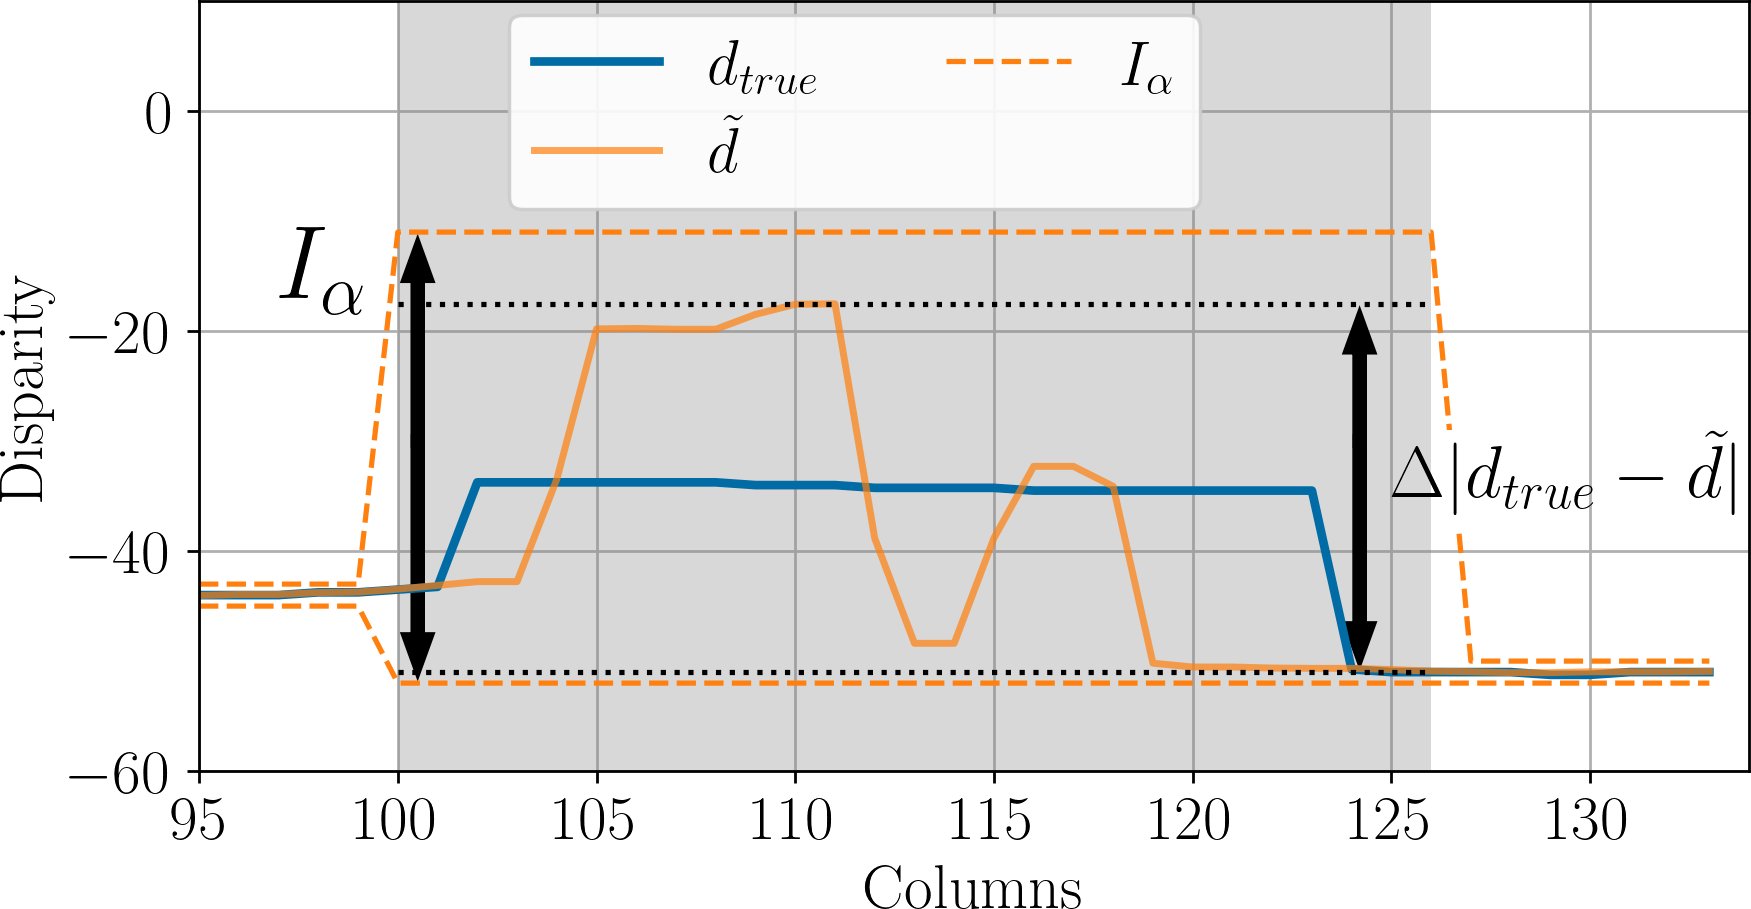
\includegraphics[width=0.8\linewidth]{Images/Chap_5/relative_overestimation_row_230.png}
    \caption{$\Delta|d_{true}-\tilde{d}|$ and $I_\alpha$ for computing the relative estimation (\cref{eq:relative_overestimation_disparity}) over a low confidence area in gray.}
    \label{fig:relative_overestimation}
\end{figure}

\begin{figure}
    \centering
    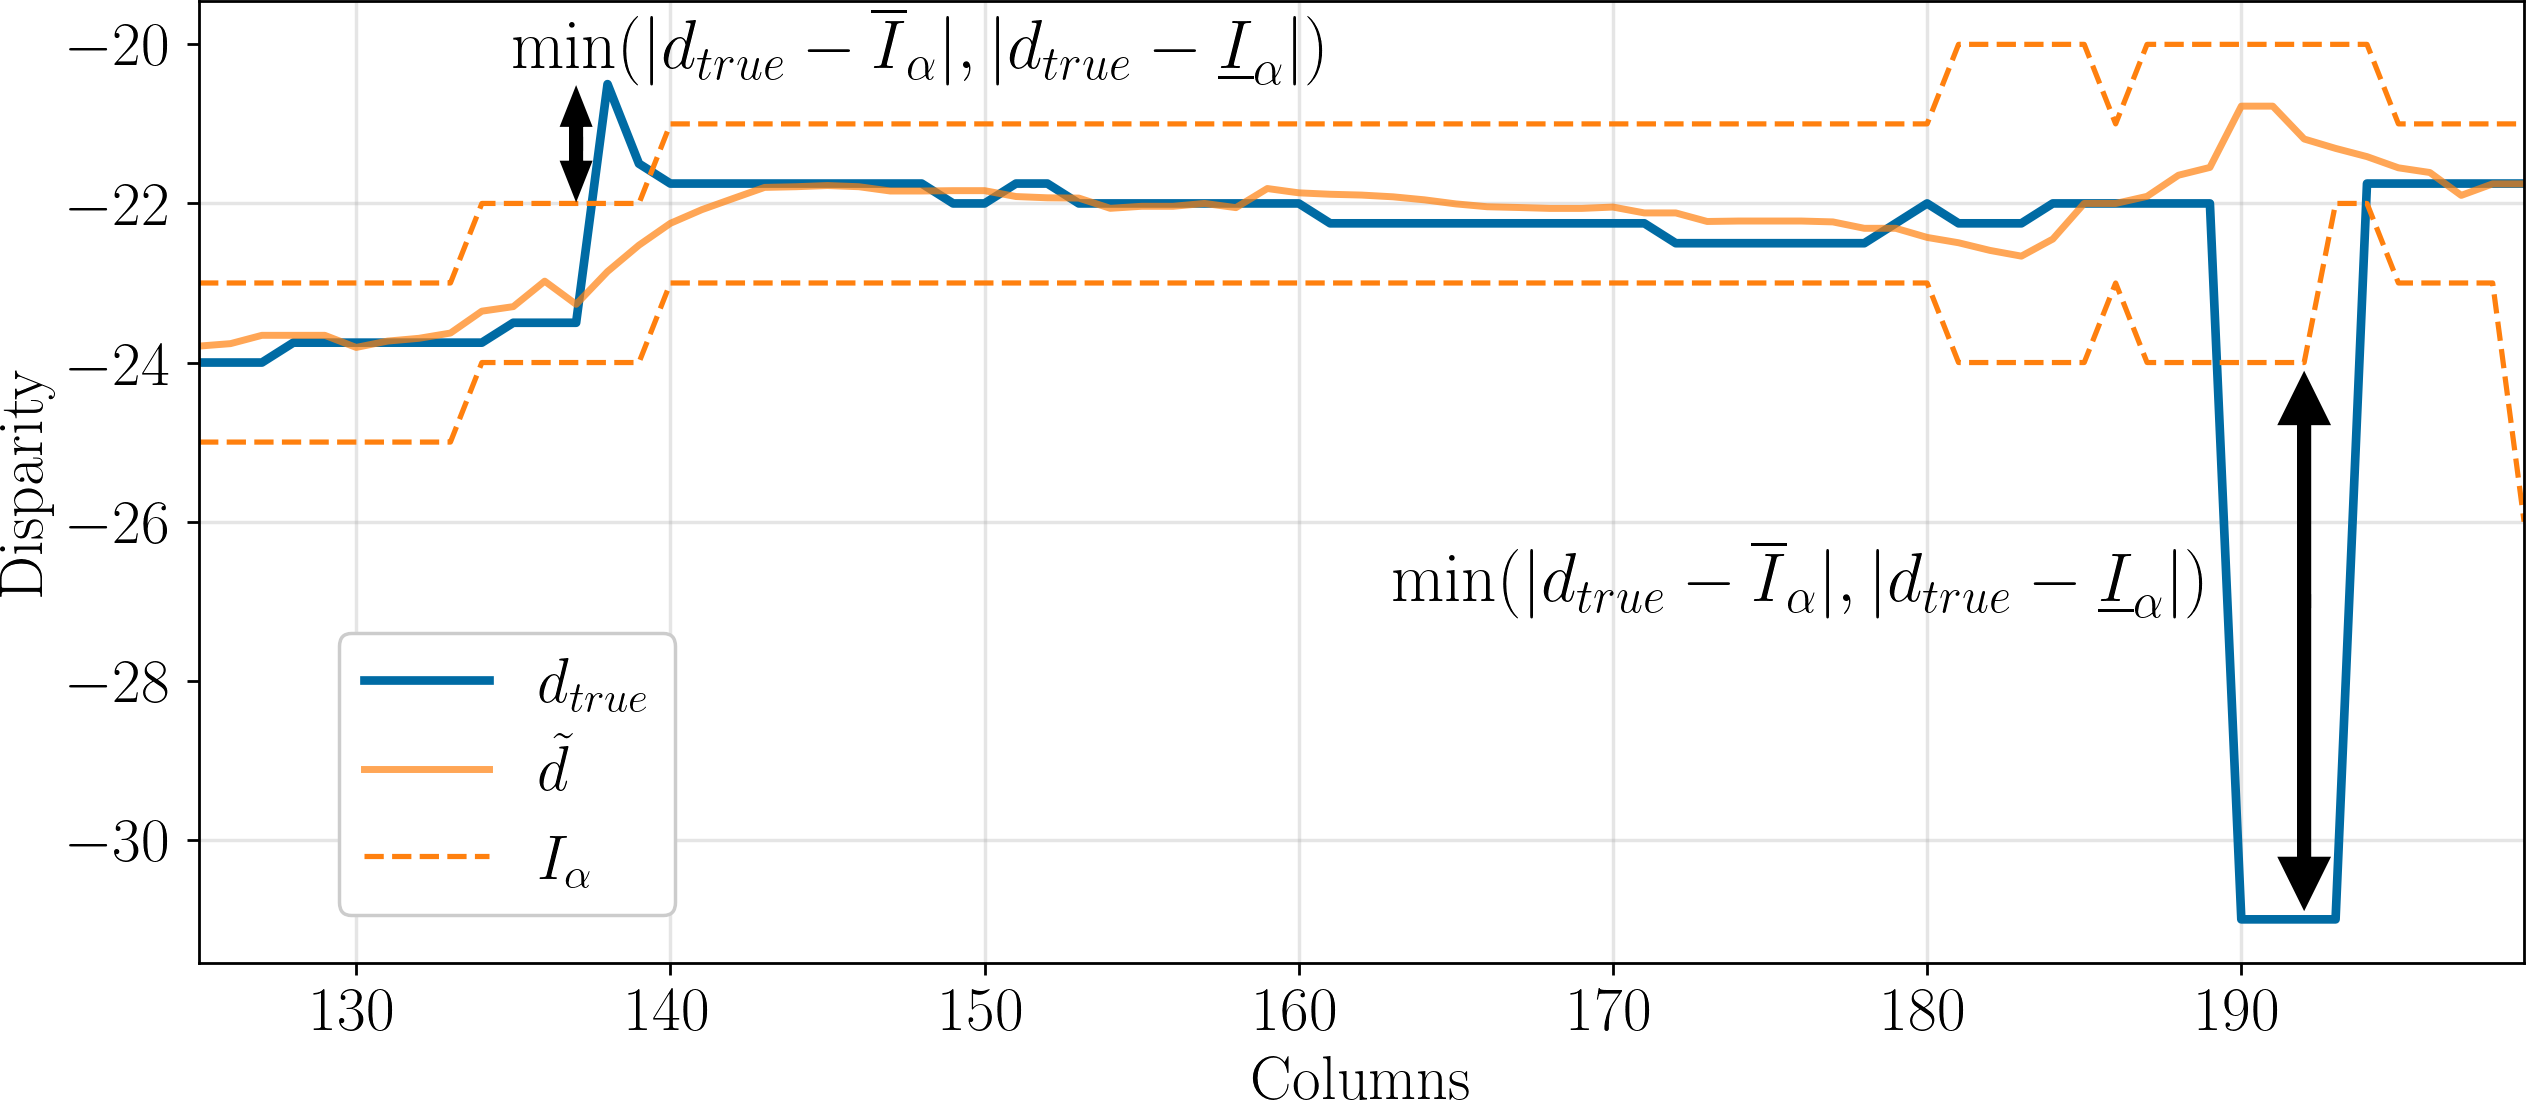
\includegraphics[width=0.8\linewidth]{Images/Chap_5/residual_error_row_108.png}
    \caption{Different values of $\min(|d_{true}-\overline{I}_\alpha|, |d_{true}-\underline{I}_\alpha|)$ for computing the residual error of \cref{eq:residual_error}}
    \label{fig:residual_error}
\end{figure}

Because we evaluate the size of intervals using two different metrics depending if intervals are in low confidence areas or not, it is interesting to measure the proportion of low confidence areas in the scene $p_{amb}$:
\begin{align}
    p_{amb} = \dfrac{\#\{I_\alpha ~|~I_\alpha\in\mathrm{low~confidence~area}\}}{\#\{I_\alpha\}}
\end{align}
A proportion $p_{amb}$ of intervals size will be evaluated using $o_{rel}$, and a proportion $1-p_{amb}$ using $s_{rel}$. A high $p_{amb}$ thus indicates many regularization and consequently larger intervals in general.

Before measuring the precision of intervals using $acc$, to quantify their errors using $\varepsilon$ or measuring their relative size with $s_{rel}$ and $o_{rel}$, we will present the different considered datasets used for our evaluation.

\subsection{Stereo Matching Dataset}\label{sec:dataset}
We evaluate the disparity confidence intervals on $76$ scenes from the Middlebury datasets. Those datasets are composed of two stereo images of indoor scenes, for which the true disparity is known with precision. It is separated on different years: 2003, 2005, 2006, 2014 and 2021 \cite{scharstein_high-accuracy_2003, scharstein_learning_2007, hirschmuller_evaluation_2007, scharstein_high-resolution_2014}, each year presenting more complex scenes. \Cref{fig:middlebury_examples} present some scenes from each dataset.  Each dataset is available in different resolutions. We use quarter-size and third-size versions of the data for 2003, 2005 and 2006 datasets and full resolution for 2014 and 2021 datasets in order to include a diversity of resolutions in our experiments. As a result, ranges of consider disparities also vary greatly, for instance the 2014 dataset are very large (more than a thousand disparity wide), which presents a significant challenge for the SGM regularization\commanue{alors disons qu'un intervalle aussi grand c'est un challenge pour l'algorithme tout court. Pour SGM c'est plus la taille des sauts de disparités qui sont des challanges je dirais. Et si tu veux pas t'embêter tu mets de côté ta remarque}. On those scenes our stereo matching algorithm performs far less well than on the 2003 dataset. This will allow to evaluate whether or not the disparity confidence intervals can perform well even when the main disparity prediction does not. Each dataset does not contain the same number of images, and shapes of images can vary across datasets and inside each datasets. For indication purposes, datasets 2003, 2005, 2006, 2014 and 2021 respectfully contain 2, 6, 21, 23 and 25 scenes.

\begin{figure}
    \centering
    \begin{subfigure}[t]{0.33\linewidth}
        \centering
        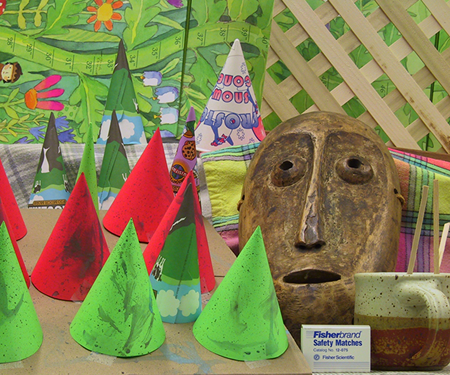
\includegraphics[width=\linewidth]{Images/Chap_5/2003cones.png}
        \caption{2003 Cones}
        \label{fig:2003_cones}
    \end{subfigure}\hfill
    \begin{subfigure}[t]{0.33\linewidth}
        \centering
        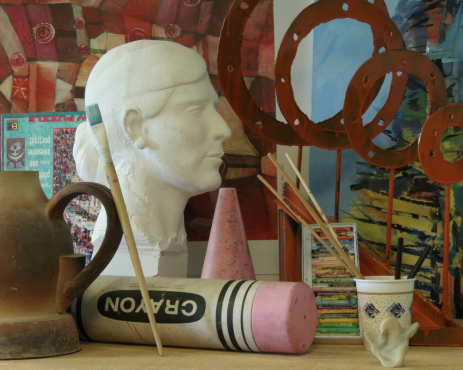
\includegraphics[width=\linewidth]{Images/Chap_5/2005art.png}
        \caption{2005 Art}
        \label{fig:2005_art}
    \end{subfigure}\hfill
    \begin{subfigure}[t]{0.33\linewidth}
        \centering
        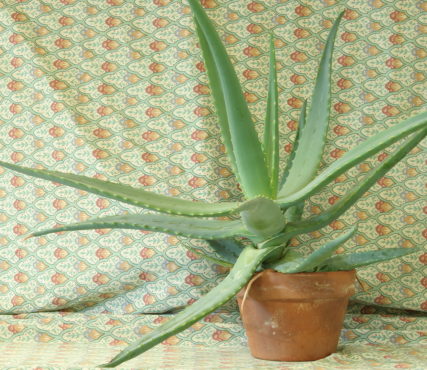
\includegraphics[width=\linewidth]{Images/Chap_5/2006aloe.png}
        \caption{2006 Aloe}
        \label{fig:2006_aloe}
    \end{subfigure}\hfill
    \begin{subfigure}[t]{0.33\linewidth}
        \centering
        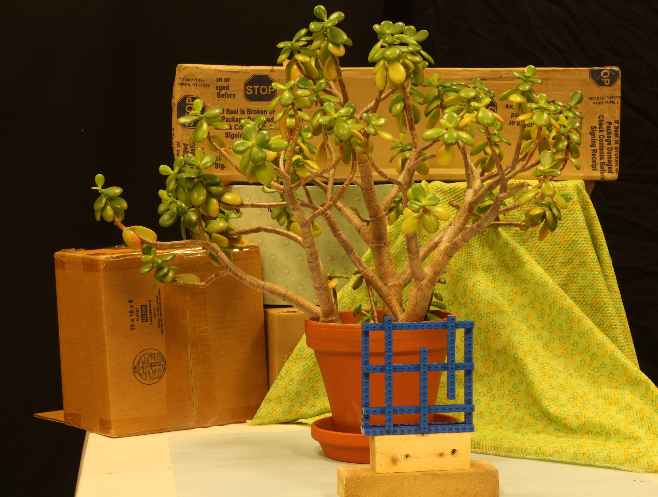
\includegraphics[width=\linewidth]{Images/Chap_5/2014_Jadeplant-perfect.png}
        \caption{2014 Jadeplant Perfect}
        \label{fig:2014_jadeplant}
    \end{subfigure}\hfill
    \begin{subfigure}[t]{0.33\linewidth}
        \centering
        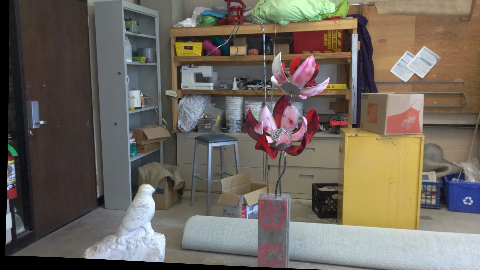
\includegraphics[width=\linewidth]{Images/Chap_5/2021_artroom1.png}
        \caption{2021 Artroom1}
        \label{fig:2021_artroom1}
    \end{subfigure}\hfill
    \begin{subfigure}[t]{0.33\linewidth}
        \centering
        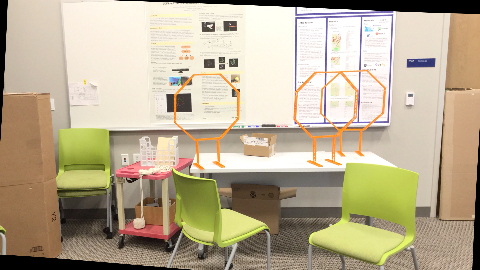
\includegraphics[width=\linewidth]{Images/Chap_5/2021_octogons1.png}
        \caption{2021 Octogons1}
        \label{fig:2021_octogons1}
    \end{subfigure}
    \caption{Example of left images from  different Middlebury datasets}
    \label{fig:middlebury_examples}
\end{figure}

The Middlebury dataset contains generic indoor scene with a high variety of 3D structures which can highlight the potential of our method for any stereo algorithm. Our objective is however to process satellite images, so we also evaluate our method on satellite data, which can greatly differ from indoor scenes. For this purpose, we use 80 pairs of $1845\times1845$ satellite images in epipolar geometry, with a typical disparity range of $[-20, 10]$ (it slightly varies between images). Those image are all part of the same pair of Pléiades images over the city of Montpellier, which is large enough to contain both urban and rural areas as presented in \Cref{fig:mtp_img}. The ground truth of those image was obtained using the method described in \cite{cournet_ground_2020}. In short, this method first process stereo images in order to get the images in epipolar geometry. Then it considers the ground truth \acrshort{dsm} of the scene, for instance some rasterized LiDAR HD data, and project it into the same geometry as one of the sensors. Then, using the disparity to altitude ratio computed alongside epipolar images, it converts the altitude of the re-projected \acrshort{dsm} into disparities. Using the same epipolar grids, this true disparity map can be projected into epipolar geometry. We now have two stereo images and their associated ``ground truth'' disparity map in epipolar geometry, ready to be processed. This method possesses a few known drawbacks: first, the ground truth is resampled in two different geometries, which relies among others on the quality of the epipolar grid. More importantly\commanue{pour moi le plsu import c'est le recalage planimétrique qu'il faut faire avant de remonter l'info LIDAR qui est le plus problématique. Après effectivement le fait que la VT présente des changements par rapport aux images induits nécessaires des erreurs supplémentaires}, the images and ground truth were acquired a few years apart which results in some new buildings being build or destroyed between images and ground truth. The vegetation also changed, so the ground truth is not $100\%$ correct. The dataset contained at first 327 pairs of images, but we detected major differences between the ground truth and the epipolar image, as illustrated in \Cref{fig:mtp_278}, so we restricted our selection to 80 pairs for which no major differences appeared. The evaluation metrics on this dataset must thus be taken with care.

\begin{figure}[ht!]
    \centering
    \begin{subfigure}[t]{0.4\linewidth}
        \centering
        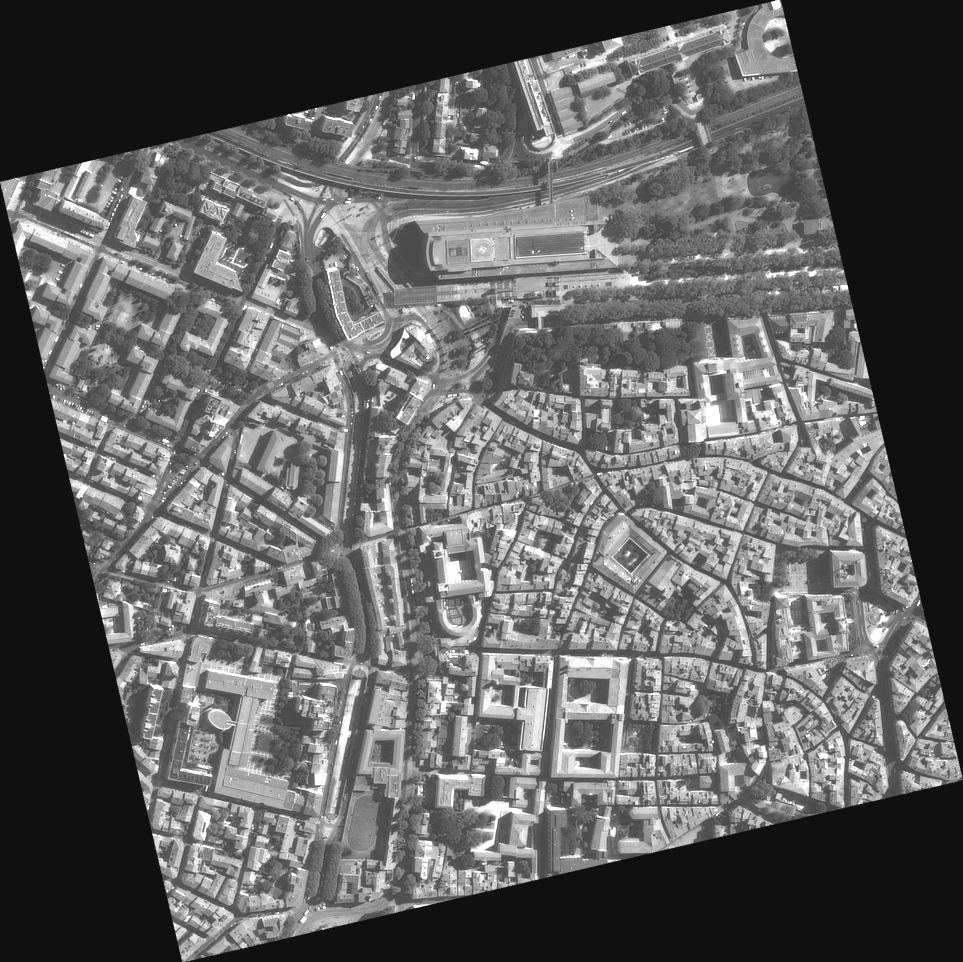
\includegraphics[width=\linewidth]{Images/Chap_5/img_MTP_120.png}
        \caption{Left epipolar image}
        \label{fig:mtp_img_a}
    \end{subfigure}\hfill
    \begin{subfigure}[t]{0.4\linewidth}
        \centering
        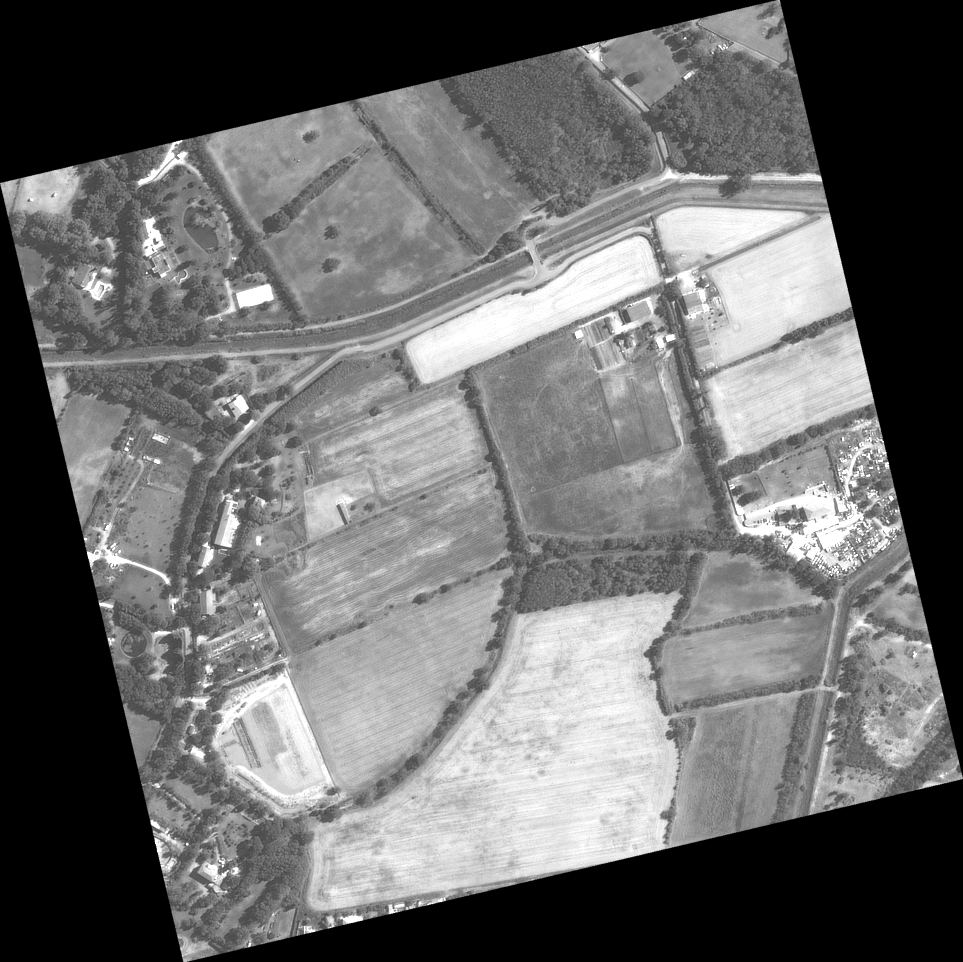
\includegraphics[width=\linewidth]{Images/Chap_5/img_MTP_153.png}
        \caption{Left epipolar image}
        \label{fig:mtp_img_b}
    \end{subfigure}\\
    \begin{subfigure}[t]{0.4\linewidth}
        \centering
        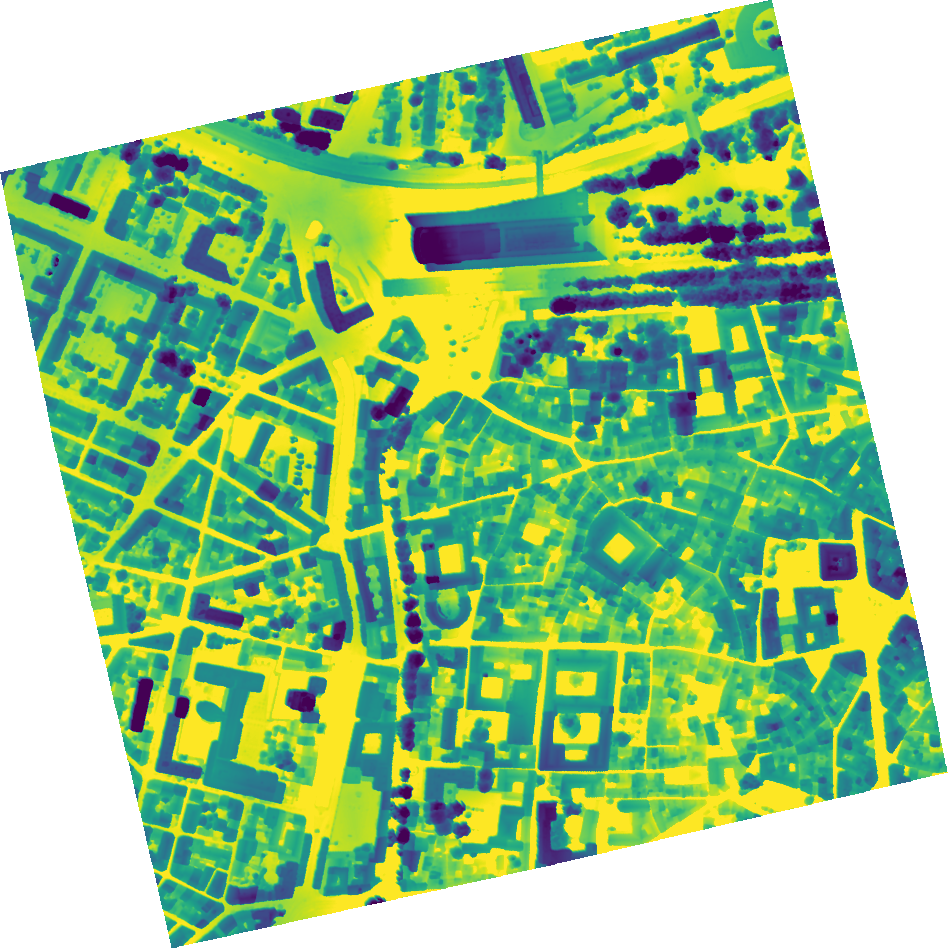
\includegraphics[width=\linewidth]{Images/Chap_5/img_MTP_120_gt.png}
        \caption{Ground truth disparity}
        \label{fig:mtp_img_c}
    \end{subfigure}\hfill
    \begin{subfigure}[t]{0.4\linewidth}
        \centering
        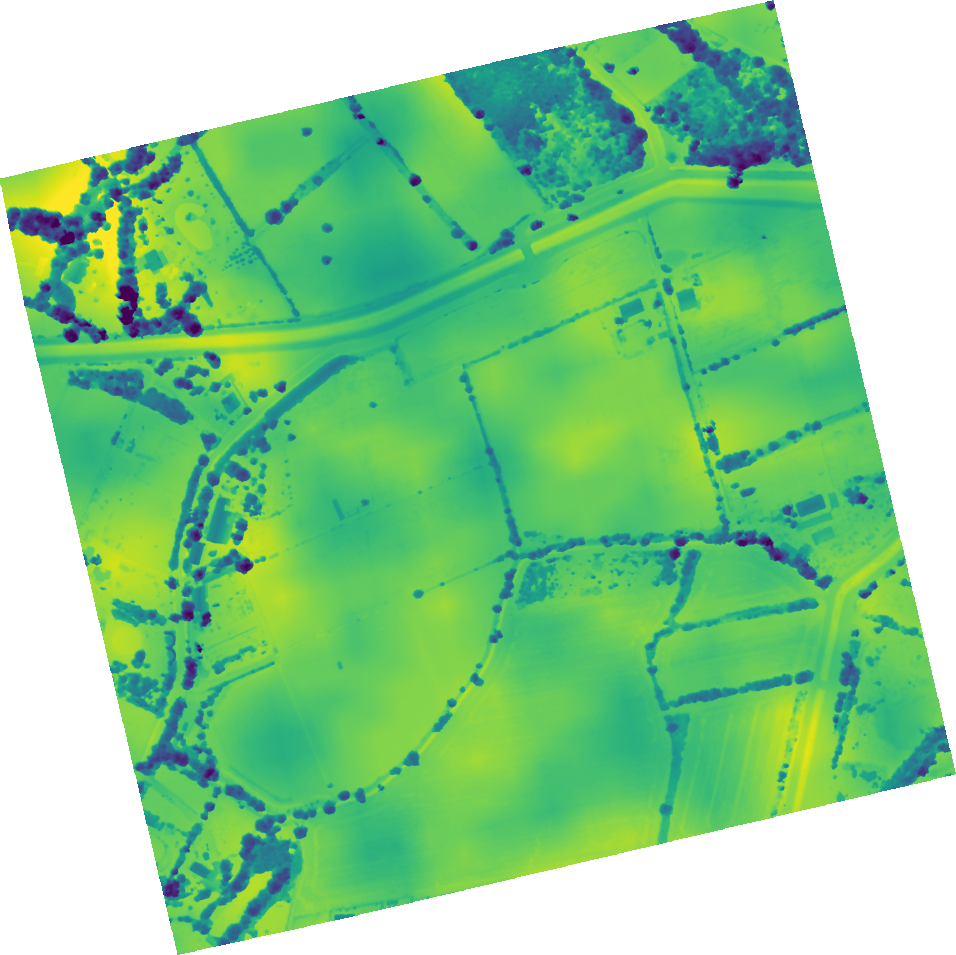
\includegraphics[width=\linewidth]{Images/Chap_5/img_MTP_153_gt.png}
        \caption{Ground truth disparity}
        \label{fig:mtp_img_d}
    \end{subfigure}
    \caption{One rural and one urban scene from the Montpellier dataset.} 
    \label{fig:mtp_img}
\end{figure}


\begin{figure}[ht!]
    \centering
    \begin{subfigure}[t]{0.4\linewidth}
        \centering
        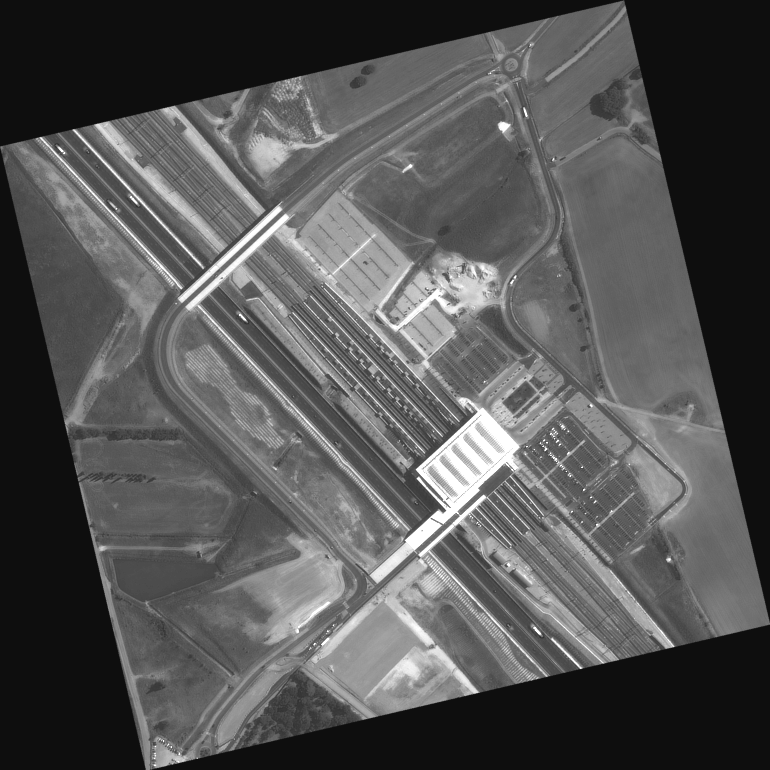
\includegraphics[width=\linewidth]{Images/Chap_5/img_error_MTP_278.png}
        \caption{Left epipolar image}
        \label{fig:mtp_278_a}
    \end{subfigure}\hfill
    \begin{subfigure}[t]{0.4\linewidth}
        \centering
        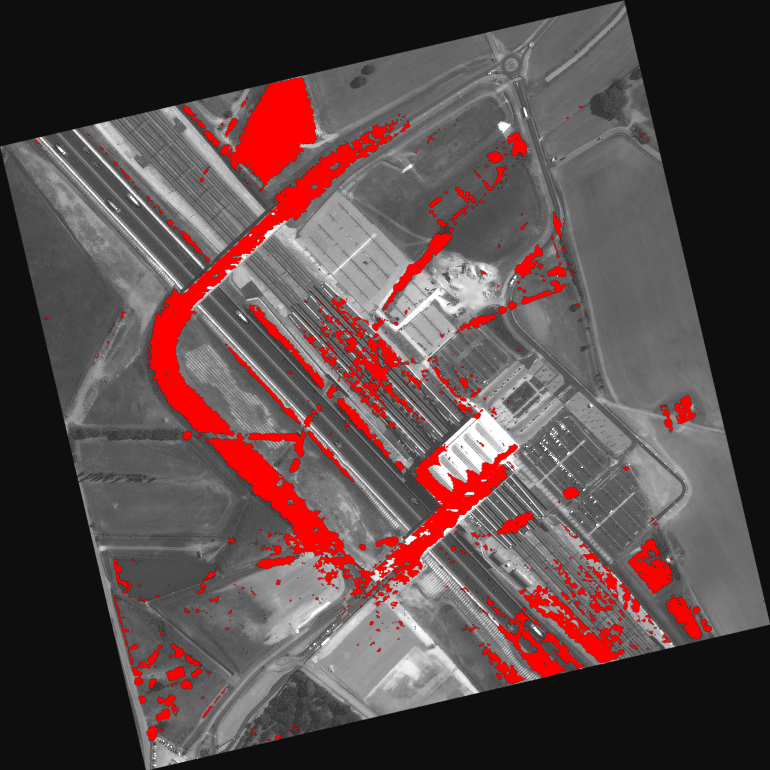
\includegraphics[width=\linewidth]{Images/Chap_5/img_error_MTP_278_err.png}
        \caption{Wrong intervals (red)}
        \label{fig:mtp_278_b}
    \end{subfigure}\\
    \begin{subfigure}[t]{0.4\linewidth}
        \centering
        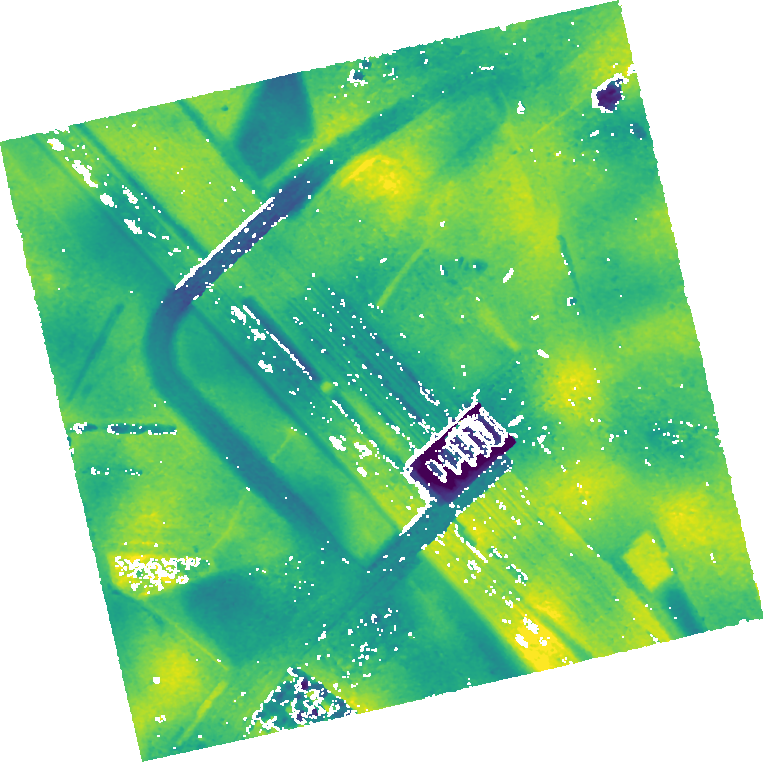
\includegraphics[width=\linewidth]{Images/Chap_5/img_error_MTP_278_disp.png}
        \caption{Predicted disparity}
        \label{fig:mtp_278_c}
    \end{subfigure}\hfill
    \begin{subfigure}[t]{0.4\linewidth}
        \centering
        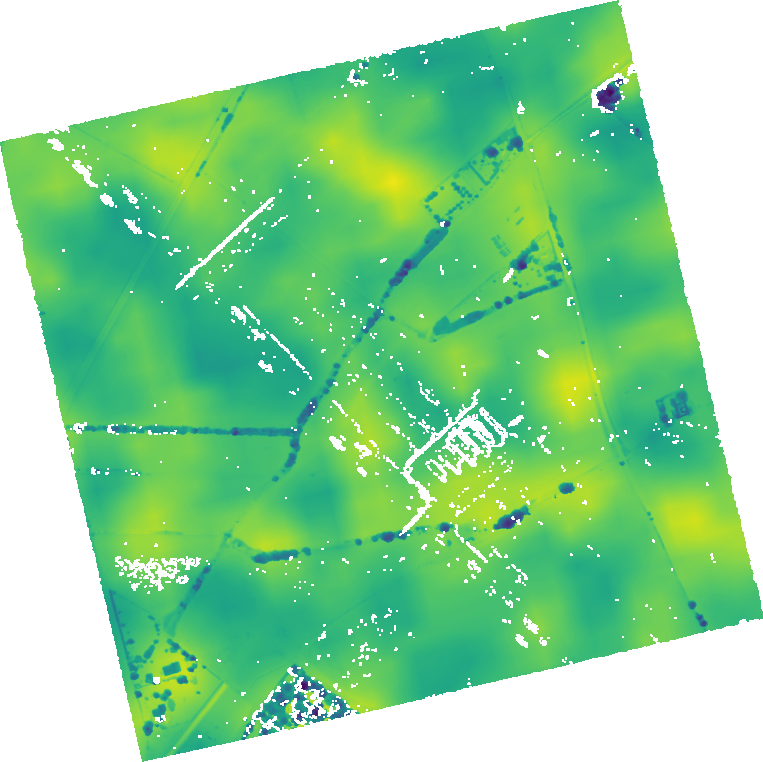
\includegraphics[width=\linewidth]{Images/Chap_5/img_error_MTP_278_gt.png}
        \caption{Ground truth}
        \label{fig:mtp_278_d}
    \end{subfigure}
    \caption{Important differences between the ground truth and the epipolar images. We can see that the road appearing in the left image from \Cref{fig:mtp_278_a} does not appear in the ground truth in \Cref{fig:mtp_278_d}, which results in false negative on the intervals from \Cref{fig:mtp_278_b}. The road must have been constructed in between the ground truth acquisition and image acquisition. Images with such differences were removed from the Montpellier dataset.} 
    \label{fig:mtp_278}
\end{figure}

In the next section, we will use the Middlebury datasets to evaluate our method on general indoor scenes, and images of Montpellier (sometimes abbreviated as $\mathrm{MTP}$) to determine if we can generalize our results to satellite imagery. We will also consider two cost functions: the CENSUS cost function and MC-CNN cost function, both detailed in \Cref{sec:cost_volume_computation} and implemented in the \acrshort{cars} pipeline\commanue{là comme tu es juste dans le corrélateur tu peux te limiter à Pandora}.

\subsection{Results}
This section will evaluate each metric on the different datasets, and for the two considered cost functions CENSUS and MC-CNN. Because there are a few metrics and many different scenes, we first give global results, and gradually go into more details across tables and figures. We first consider global results on Middlebury datasets as they are more general and possess a ground truth of better quality. Each metric is evaluated and averaged over the whole dataset (\ie 2003, 2005, 2006 \etc)\commanue{tu peux enlever l'énumération} in \Cref{tab:metric_average} to get an overall estimation of the performances. To have a better estimation of scores distribution across scenes, we then plot histograms of each metric across all datasets in \Cref{fig:acc_hist,fig:s_rel_hist,fig:o_rel_hist,fig:eps_hist}. Finally, we will also discuss the metrics by looking at some details of particular scenes.

\begin{table}[ht!]
\centering
\renewcommand{\arraystretch}{1.5}
\begin{tabular}{|c|c||c|c|c|c|c|}
\cline{2-7}
\rowcolor{lightgray}
\multicolumn{1}{c|}{\cellcolor{white}}& Year & 2003 & 2005 & 2006 & 2014 & 2021 \\ \hline

\rowcolor{color_census}
\cellcolor{white} & CENSUS & $97.6\%$ & $96.4\%$ & $99.1\%$ & $94.8\%$ & $91.6\%$\\\cline{2-7}

\rowcolor{color_mccnn}
\multirow{-2}{*}{\cellcolor{white} $acc$ $\uparrow$} & MC-CNN & $97.0\%$ & $97.5\%$ & $99.3\%$ & $98.5\%$ & $99.1\%$\\

\rowcolor{color_census}\hline
\cellcolor{white} & CENSUS & $2.5\%$ & $3.1\%$ & $5.3\%$ & $0.2\%$ & $0.9\%$\\\cline{3-7} 

\rowcolor{color_mccnn}
\multirow{-2}{*}{\cellcolor{white} $\varepsilon_{~~~}$ $\downarrow$} & MC-CNN & $4.0\%$ & $5.6\%$ & $10.0\%$ & $3.8\%$ & $8.3\%$\\

\rowcolor{color_census}\hline
\cellcolor{white} & CENSUS & $3.3\%$ & $2.6\%$ & $2.6\%$ & $0.6\%$ & $1.2\%$\\\cline{3-7} 

\rowcolor{color_mccnn}
\multirow{-2}{*}{\cellcolor{white} $s_{rel}$ $\downarrow$} & MC-CNN & $3.3\%$ & $2.6\%$ & $3.0\%$ & $1.5\%$ & $3.3\%$\\

\rowcolor{color_census}\hline
\cellcolor{white} & CENSUS & $55.8\%$ & $66.9\%$ & $73.9\%$ & $70.9\%$ & $67.5\%$\\\cline{3-7} 

\rowcolor{color_mccnn}
\multirow{-2}{*}{\cellcolor{white} $o_{rel}$ $\downarrow$} & MC-CNN & $58.5\%$ & $71.3\%$ & $80.4\%$ & $86.3\%$ & $78.0\%$\\

\rowcolor{color_census}\hline
\cellcolor{white} & CENSUS & $20.8\%$ & $29.1\%$ & $27.1\%$ & $47.1\%$ & $59.2\%$\\\cline{3-7} 

\rowcolor{color_mccnn}
\multirow{-2}{*}{\cellcolor{white} $p_{amb}$} & MC-CNN & $15.3\%$ & $41.1\%$ & $39.9\%$ & $43.2\%$ & $69.1\%$\\\hline


\end{tabular}
\renewcommand{\arraystretch}{1}
\caption{Average metrics over the different Middlebury datasets, depending on the cost function. Up arrows indicate that the optimal score is $100\%$, and $0\%$ for down arrows. $amb$ is the proportion of low confidence area, computed with the ambiguity.}\label{tab:metric_average}
\end{table}

In \Cref{tab:metric_average}, each metric is evaluated and averaged over each Middlebury dataset: 2003 to 2021\commanue{Si jamais tu as la stat ça peut être bien d'avoir le pourcentage de disparté valide (< à seuil de 1)}. The conclusions drawn for this table are quite general as we are looking at averages across multiple datasets. We will dive into more details later in this section. Here are some of the key takeaways from this table:
\begin{itemize}
    \item Accuracy $acc$: the first observation is that the accuracy is greater than the $90\%$ objective on each dataset, and for both considered cost curve\commanue{function?}. In fact, the average is always higher than $91.6\%$, and reaches $99.3\%$ accuracy on some datasets (2006 with MC-CNN). Except for the $2003$ dataset it seems that intervals computed using the MC-CNN cost curves\commanue{just MC-CNN?} are more accurate than those using CENSUS. This high accuracy must however be considered along side the size of the intervals with $s_{rel}$ and $o_{rel}$.
    
    \item Residual error $\varepsilon$: residual errors values are between $0.2\%$ and $10\%$ for all datasets, which is relatively low. The residual error is always lower for CENSUS intervals than for MC-CNN ones. In particular, the residual error using CENSUS is almost ten times smaller than that using MC-CNN for the 2021 dataset. This means that it is easier to improve the accuracy of CENSUS intervals, as they miss the true disparity by a smaller fraction of disparity range, than MC-CNN intervals. With the conclusions drawn from the accuracy results, it seems that the last few missing accuracy percent are the hardest to recover.
    
    \item Relative size $s_{rel}$: The relative size of intervals in high confidence areas is relatively low. Across datasets, it is on average between $0.6\%$ and $3.3\%$. This broadly means that half of intervals sizes (in high confidence areas) are less than $5\%$ of the considered disparity range. This is a very reasonable size for confidence intervals. For datasets 2003 to 2006, both cost functions lead to similar relative sizes. For datasets 2014 and 2021, the MC-CNN cost curves leads to larger intervals around 3 times bigger than the CENSUS intervals. This is coherent with the higher accuracy of MC-CNN intervals on those datasets.
    
    \item Relative over-estimation $o_{rel}$: The range of relative over-estimation of intervals across datasets is more widely spread. It ranges between $46.8\%$ and $72.6\%$. Except for the 2003 dataset, the MC-CNN cost functions clearly leads to intervals with higher over-estimation than those obtained using the CENSUS cost function. CENSUS intervals typically overestimate intervals in low confidence areas by around $50\%$, while it is around $60\%$ or $70\%$ for MC-CNN intervals. This means that half or low confidence pixels have $50\%$ or less of their size that is superfluous when using CENSUS, but for MC-CNN the proportion of superfluous size reaches $60\%$ to $70\%$. For CENSUS, this score is around what we deem\commanue{donc tu as des synonymes à consider en fait ;)} to be a good performing intervals. For MC-CNN, it seems to be a bit large. We must however take into consideration the complexity of datasets 2014 and 2021. Indeed, we will see in some examples that the correlator has a hard time producing a good quality disparity map for some scenes, and that over-estimating the intervals is necessary to produce accurate intervals (for instance in \Cref{fig:sword2}).
    
    \item Proportion of low confidence area $p_{amb}$: \Cref{tab:metric_average} also indicates the proportion of low confidence areas. This provides indicative insights on the proportion of intervals that have been evaluated using $o_{rel}$, the rest being evaluated using $s_{rel}$. It is hard to see whether or not there is a cost function leading to more low confidence areas than the other, and the proportion of low confidence area do not seem to be correlated to the accuracy or to the residual error.
\end{itemize}

\begin{figure}
    \centering
    \begin{subfigure}[t]{0.5\linewidth}
        \centering
        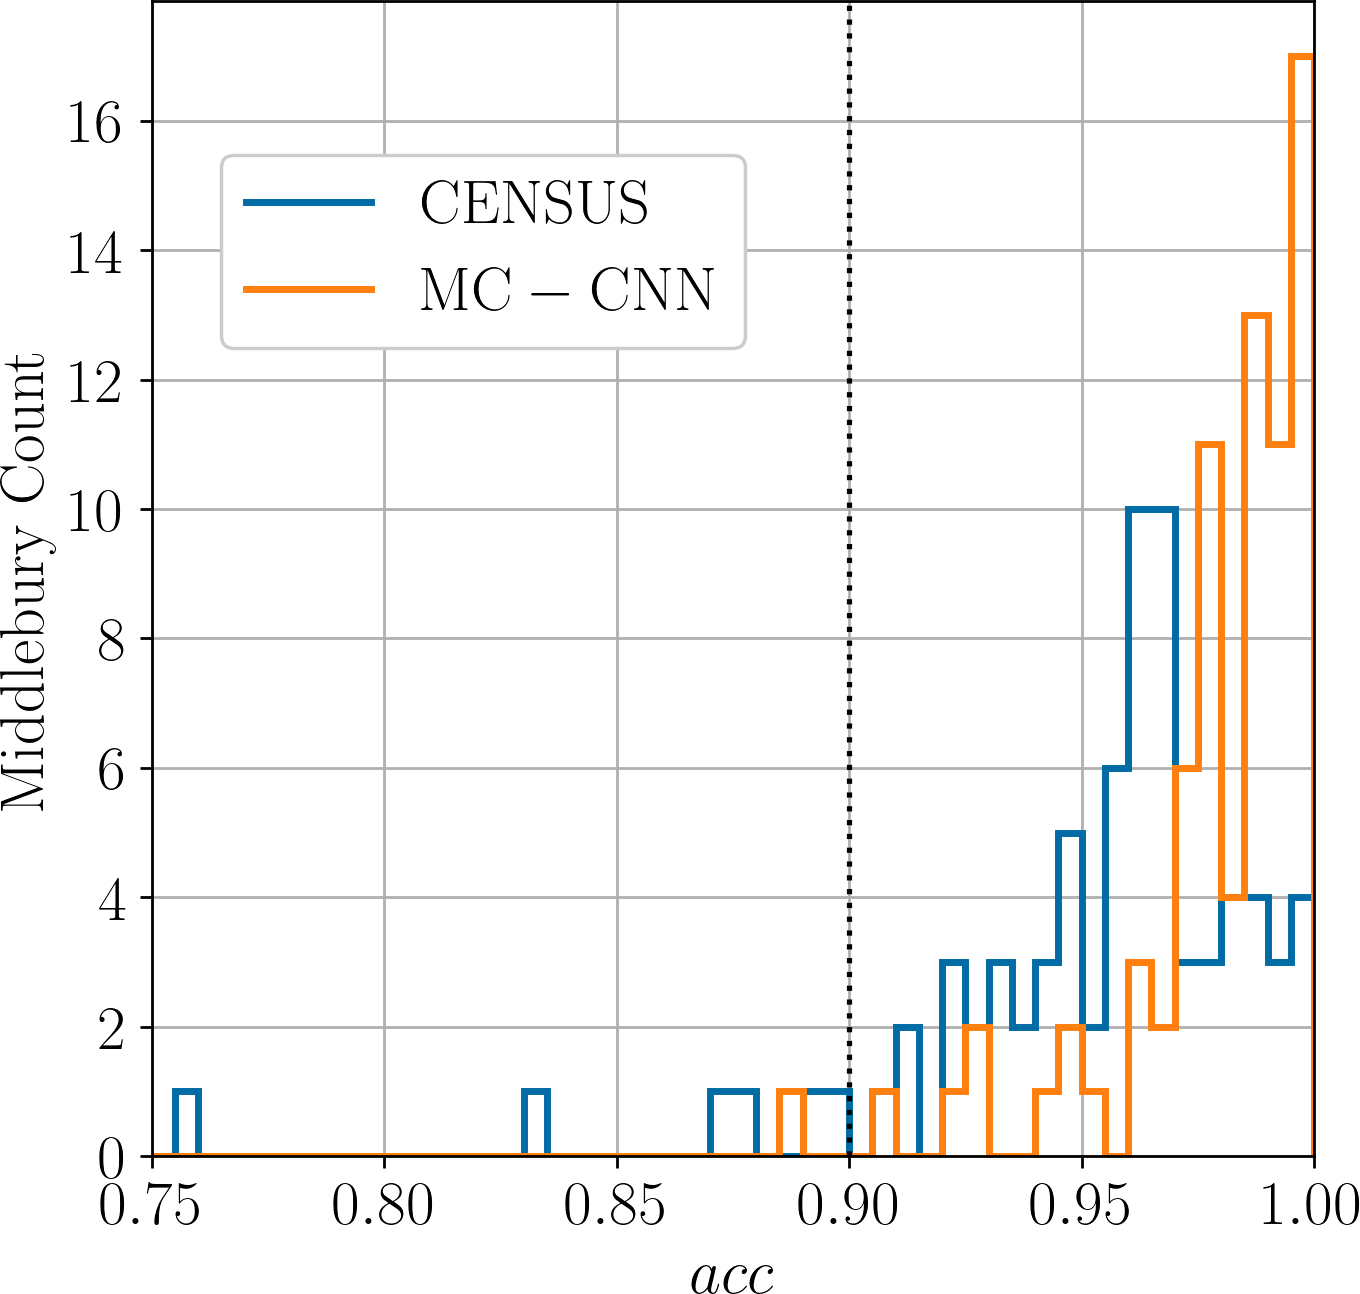
\includegraphics[width=\linewidth]{Images/Chap_5/histogram_acc_middlebury.png}
        \caption{Middlebury}
        \label{fig:acc_middlebury}
    \end{subfigure}\hfill
    \begin{subfigure}[t]{0.5\linewidth}
        \centering
        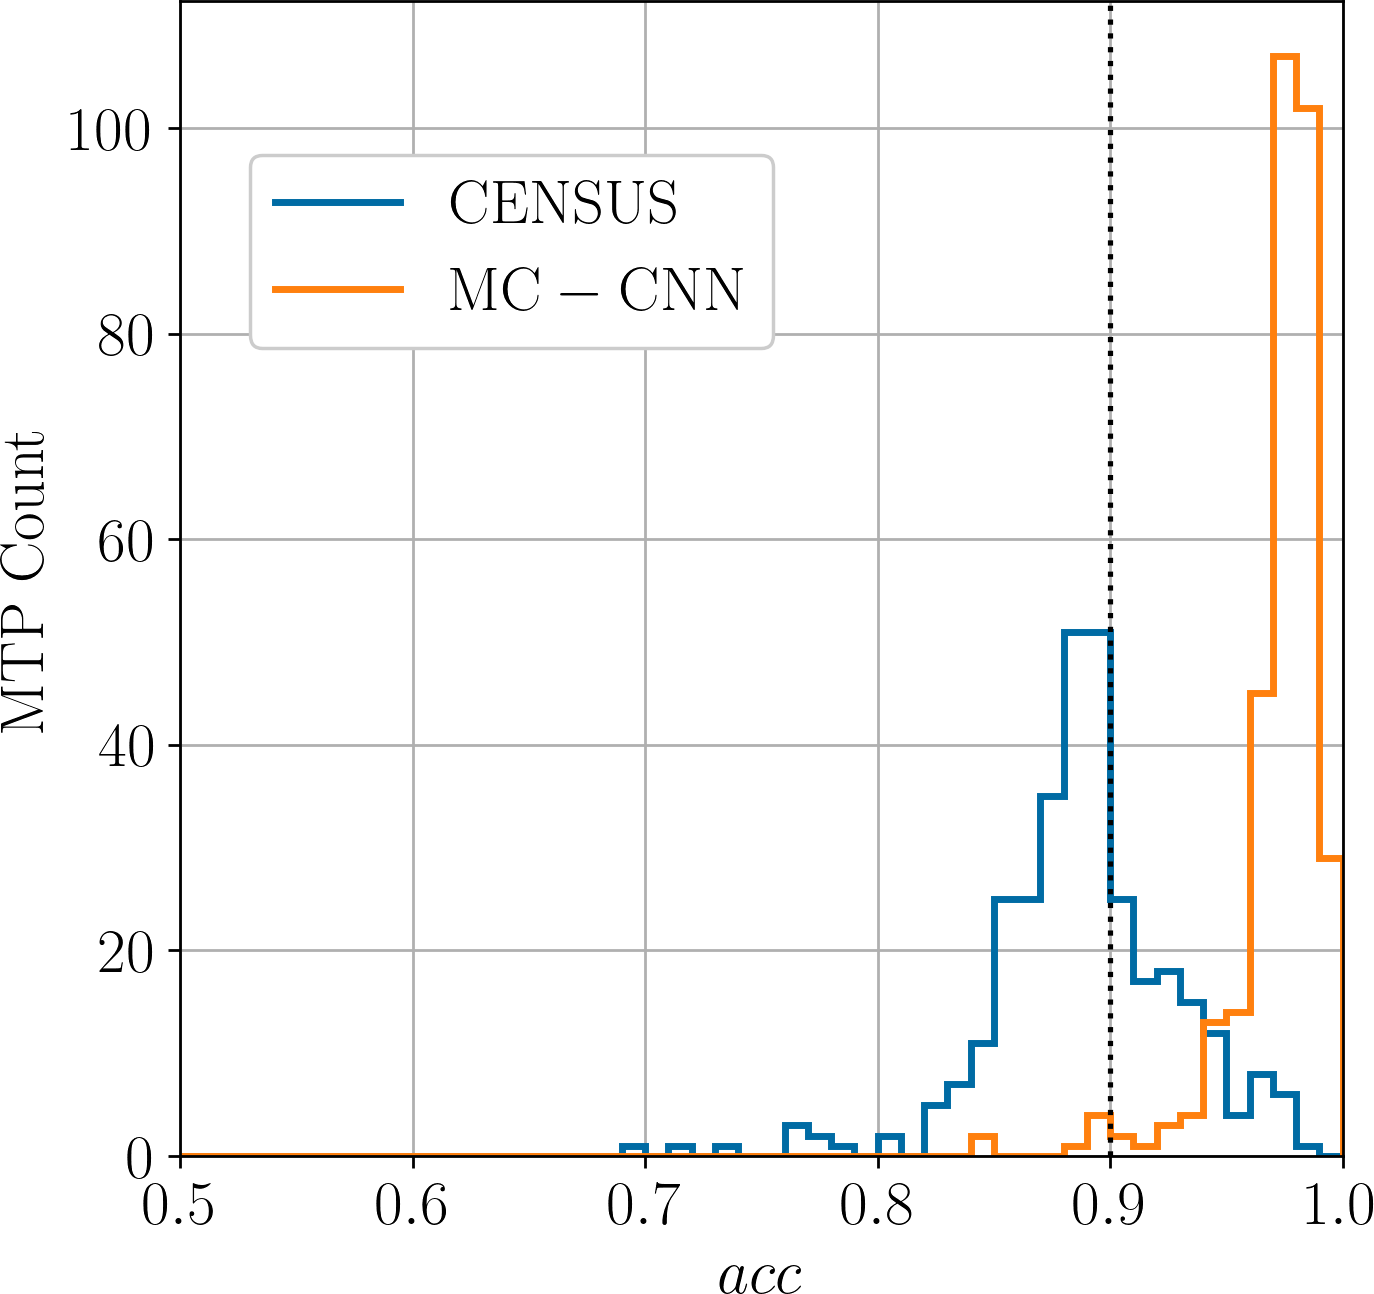
\includegraphics[width=\linewidth]{Images/Chap_5/histogram_acc_mtp.png}
        \caption{Montpellier}
        \label{fig:acc_mtp}
    \end{subfigure}
    \caption{Accuracy $acc$ histograms over the different datasets depending on the cost function. Each histogram counts the number of scenes. The vertical dotted line represent the $90\%$ objective.}
    \label{fig:acc_hist}
\end{figure}

\begin{figure}
    \centering
    \begin{subfigure}[t]{0.5\linewidth}
        \centering
        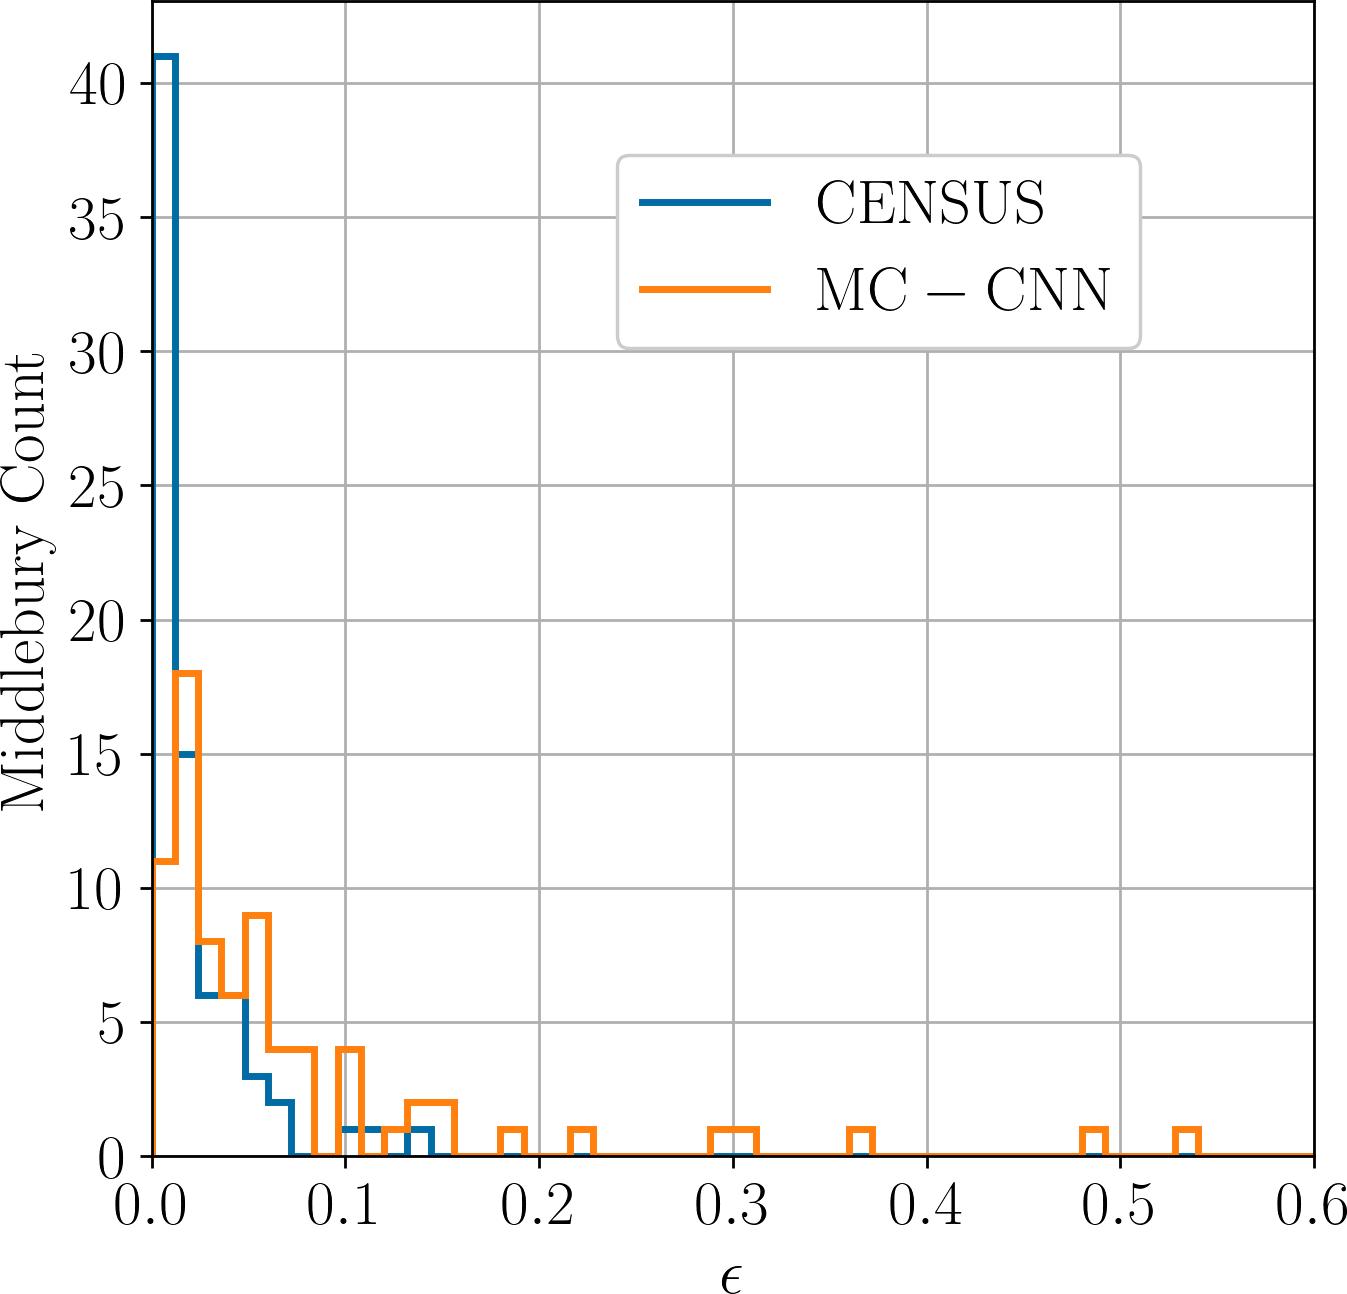
\includegraphics[width=\linewidth]{Images/Chap_5/histogram_eps_middlebury.png}
        \caption{Middlebury}
        \label{fig:eps_middlebury}
    \end{subfigure}\hfill
    \begin{subfigure}[t]{0.5\linewidth}
        \centering
        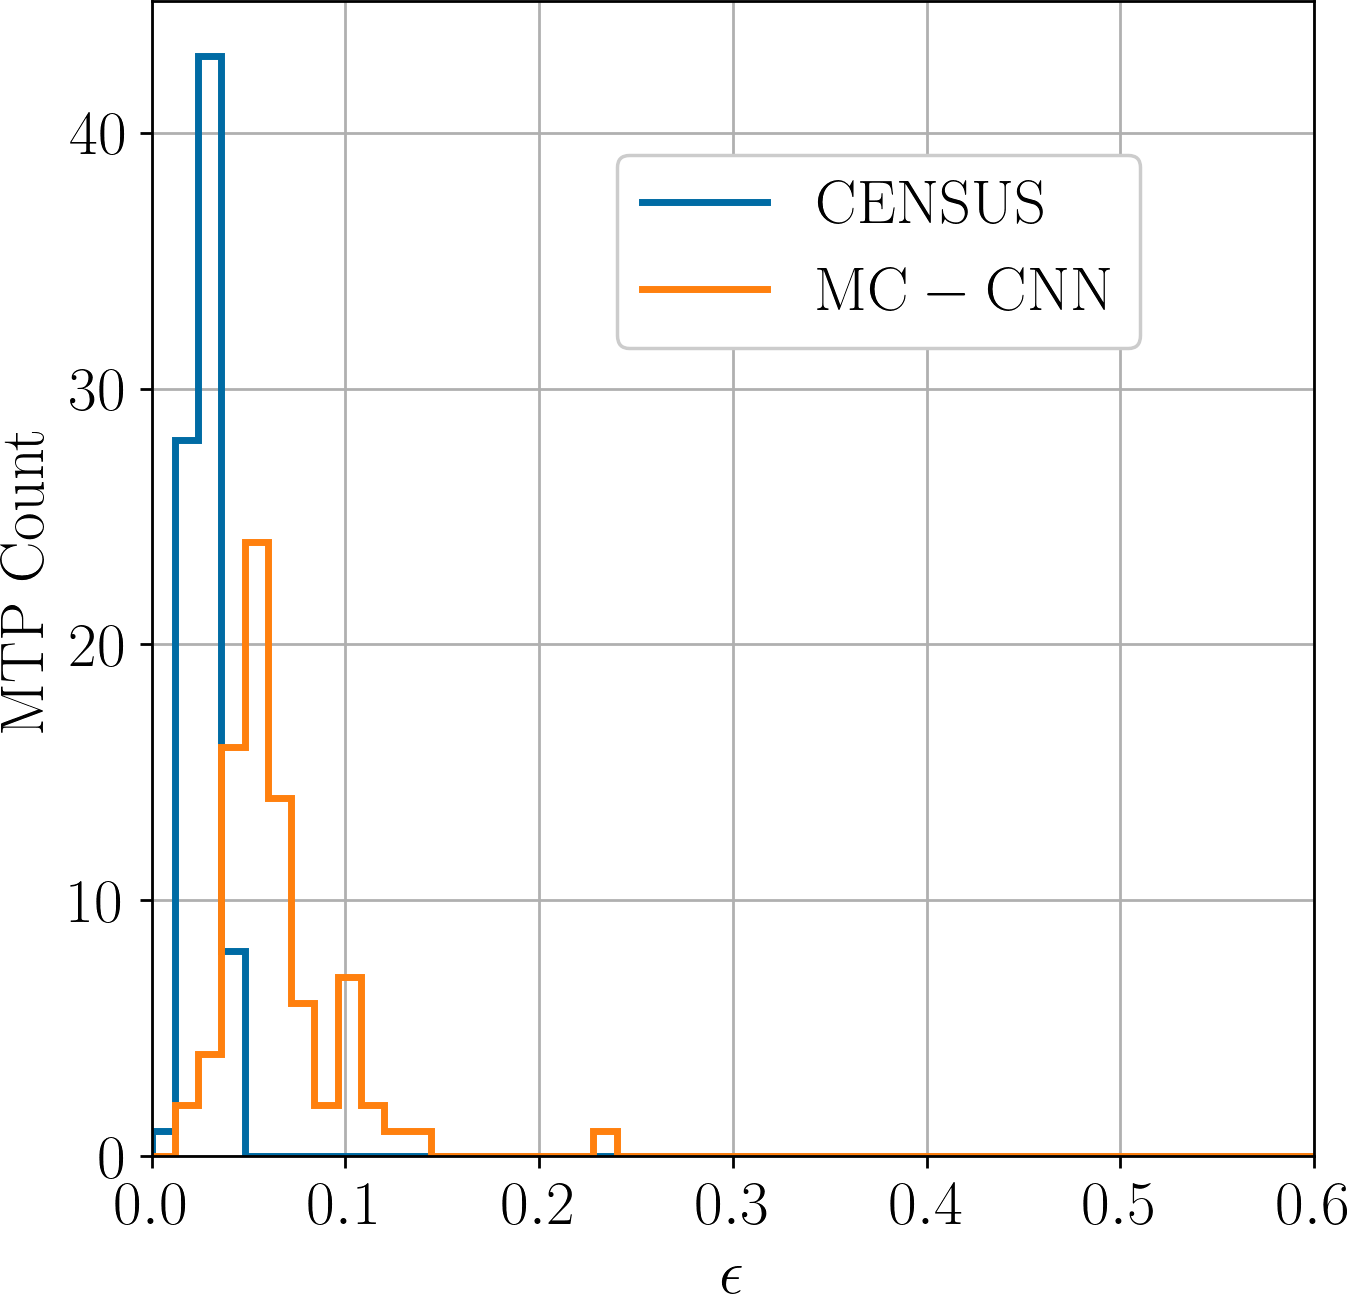
\includegraphics[width=\linewidth]{Images/Chap_5/histogram_eps_mtp.png}
        \caption{Montpellier}
        \label{fig:eps_mtp}
    \end{subfigure}
    \caption{Residual error $\varepsilon$ histograms over the different datasets depending on the cost function. Each histogram counts the number of scenes.}
    \label{fig:eps_hist}
\end{figure}

We have a good first estimation of the performance of the method for creating confidence disparity intervals. We can now dive more into details by looking at the distribution of score across all scenes, for the Middlebury datasets and the Montpellier images separately. The results are presented in \Cref{fig:acc_hist,fig:s_rel_hist,fig:o_rel_hist,fig:eps_hist}. \Cref{fig:acc_middlebury} presents the accuracy distribution across all Middlebury scenes. For the CENSUS cost function, there are in total 9 scenes across the 76 Middlebury images that do not verify the $90\%$ accuracy threshold, 4 of which have an accuracy greater\commanue{less?} than $89\%$. Those scenes are all taken from the 2014 and 2021 datasets, which are complex scenes with very large disparity intervals, typically not found in the stereo satellites image we consider for building the \acrshort{dsm}. Intervals using the MC-CNN cost function all verify the $90\%$ accuracy threshold.


\begin{figure}
    \centering
    \begin{subfigure}[t]{0.5\linewidth}
        \centering
        \includegraphics[width=\linewidth]{Images/Chap_5/histogram_s_rel_middlebury.png}
        \caption{Middlebury}
        \label{fig:s_rel_middlebury}
    \end{subfigure}\hfill
    \begin{subfigure}[t]{0.5\linewidth}
        \centering
        \includegraphics[width=\linewidth]{Images/Chap_5/histogram_s_rel_mtp.png}
        \caption{Montpellier}
        \label{fig:s_rel_mtp}
    \end{subfigure}
    \caption{Relative size $s_{rel}$  histograms over the different datasets depending on the cost function. Each histogram counts the number of scenes.}
    \label{fig:s_rel_hist}
\end{figure}

\Cref{fig:acc_hist,fig:eps_hist,fig:s_rel_hist,fig:o_rel_hist} provides more details on the distribution of each metric across Middlebury scenes and Montpellier scenes\commanue{Alors là il y a des redites entre ce paragraphe et le précédent, donc à fusionner}. Regarding the Middlebury datasets, those figures support observations made in \Cref{tab:metric_average}, as the distribution of most metrics are concentrated around the same values. Regarding the accuracy using the CENSUS cost function, there are in total 9 scenes across the 76 Middlebury images that do not verify the $90\%$ accuracy threshold, 4 of which have however an accuracy greater\commanue{less?} than $89\%$. Those scenes are all from the 2014 and 2021 datasets, which are complex scenes with very large disparity intervals, typically not found in the stereo satellites image we consider for building the \acrshort{dsm}. Intervals using the MC-CNN cost function all verify the $90\%$ accuracy threshold. Another noteworthy remark concerns the relative over-estimation: CENSUS intervals values are concentrated around $50\%$ but spread almost across the entire range, while MC-CNN intervals are more uniformly distributed along values in $[0.4, 0.9]$. This does not change the observation that using the MC-CNN cost function leads to a greater over-estimation of intervals than using the CENSUS cost function\commanue{Pour Middlebury j'ai l'impression que tu ne mentionnes que la métrique $acc$ et $o_{rel}$ donc tu ne commentes pas toutes les courbes}. 

The differences between CENSUS intervals and MC-CNN intervals are also observed on the Montpellier dataset. The $90\%$ accuracy objective is respected, and MC-CNN intervals are more accurate in general. Their residual error, relative size and relative over-estimation are all larger than those of CENSUS intervals. In general, the residual error, relative size and relative over-estimation on the Montpellier dataset are greater than on the Middlebury datasets, while still remaining relatively low. This is due to the smaller disparity range for those images (typically $[-20, 10]$) in compared to Middlebury ranges. 

\begin{remark}\commanue{peut-être éventuellement rappeler au début du chapitre le paramétrage...}
    MC-CNN cost function generates larger intervals than the CENSUS cost function, but they are more accurate in consequence. Tuning different parameters in our method could lead to the same performances of the two cost functions, but this was not explored as our primary objective is to propagate the disparity intervals to the rest of the photogrammetry pipeline.
\end{remark}


\begin{figure}
    \centering
    \begin{subfigure}[t]{0.5\linewidth}
        \centering
        \includegraphics[width=\linewidth]{Images/Chap_5/histogram_o_rel_middlebury.png}
        \caption{Middlebury}
        \label{fig:o_rel_middlebury}
    \end{subfigure}\hfill
    \begin{subfigure}[t]{0.5\linewidth}
        \centering
        \includegraphics[width=\linewidth]{Images/Chap_5/histogram_o_rel_mtp.png}
        \caption{Montpellier}
        \label{fig:o_rel_mtp}
    \end{subfigure}
    \caption{Relative over-estimation $o_{rel}$ histograms over the different datasets depending on the cost function. Each histogram counts the number of scenes.}
    \label{fig:o_rel_hist}
\end{figure}

We evaluated the metrics quantitatively across datasets and scenes in \Cref{tab:metric_average,fig:acc_hist,fig:eps_hist,fig:s_rel_hist,fig:o_rel_hist}\commanue{alors ta macro met pas de F majuscule à Figure}. Those analysis gave us a global overview of the performances\commanue{remarque générale faite au milieu de la section mais vérifie que performance en anglais se met bien au pluriel comme en français.} of the intervals. However, providing a quantitative analysis on \textit{local} performances is more complex and tedious. We instead present a qualitative analysis of the intervals in \Cref{fig:piano,fig:mtp_291}. The accuracy can be observed on \Cref{fig:piano_b,fig:mtp_291_b}, as the proportion of red pixels (indicating wrong intervals) is relatively low. The size of intervals in high confidence areas can be estimated by looking at pixels from columns 900 to 950 of \Cref{fig:piano_c} or columns 700 to 800 of \Cref{fig:mtp_291_b}. They seem to be around 2 disparities wide, which is quite small. In low confidence areas, for instance near column 850 of \Cref{fig:piano_c} and column 830 of \Cref{fig:mtp_291_c}, intervals do not over-estimate to much the maximum potential error between the predicted disparity and the true disparity. \Cref{fig:sword2} illustrates a case where the stereo matching algorithm has very poor performances of when it comes to the disparity prediction. Most areas are low confidence areas, and the predicted disparity is sometimes hundred of pixels apart from the true disparity. However, the intervals are still correct, although they are necessarily very large.  

\begin{figure}
    \centering
    \begin{subfigure}[t]{0.5\linewidth}
        \centering
        \includegraphics[width=\linewidth]{Images/Chap_5/Piano-perfect_2014.png}
        \caption{Left Image}
        \label{fig:piano_a}
    \end{subfigure}\hfill
    \begin{subfigure}[t]{0.5\linewidth}
        \centering
        \includegraphics[width=\linewidth]{Images/Chap_5/Piano-perfect_2014_error.png}
        \caption{Wrong intervals (red)}
        \label{fig:piano_b}
    \end{subfigure}\\
    \begin{subfigure}[t]{1\linewidth}
        \centering
        \includegraphics[width=\linewidth]{Images/Chap_5/Piano-perfect_2014_row_900.png}
        \caption{True disparity, predicted disparity and intervals along the blue line of \Cref{fig:piano_b}. Gray areas represent low confidence areas.}
        \label{fig:piano_c}
    \end{subfigure}
    \caption{``Piano'' scene from Middlebury 2014 dataset.}
    \label{fig:piano}
\end{figure}

\begin{figure}
    \centering
    \begin{subfigure}[t]{0.5\linewidth}
        \centering
        \includegraphics[width=\linewidth]{Images/Chap_5/MTP_291.png}
        \caption{Left Image}
        \label{fig:mtp_291_a}
    \end{subfigure}\hfill
    \begin{subfigure}[t]{0.5\linewidth}
        \centering
        \includegraphics[width=\linewidth]{Images/Chap_5/MTP_291_error.png}
        \caption{Wrong intervals (red)}
        \label{fig:mtp_291_b}
    \end{subfigure}\\
    \begin{subfigure}[t]{1\linewidth}
        \centering
        \includegraphics[width=\linewidth]{Images/Chap_5/MTP_291_error_row_750.png}
        \caption{True disparity, predicted disparity and intervals along the blue line of \Cref{fig:mtp_291_b}. Gray areas represent low confidence areas.}
        \label{fig:mtp_291_c}
    \end{subfigure}
    \caption{Scene from the Montpellier dataset.}
    \label{fig:mtp_291}
\end{figure}

\begin{figure}
    \centering
    \begin{subfigure}[t]{0.5\linewidth}
        \centering
        \includegraphics[width=\linewidth]{Images/Chap_5/Sword2-perfect_2014.png}
        \caption{Left Image}
        \label{fig:sword2_a}
    \end{subfigure}\hfill
    \begin{subfigure}[t]{0.5\linewidth}
        \centering
        \includegraphics[width=\linewidth]{Images/Chap_5/Sword2-perfect_2014_error.png}
        \caption{Wrong intervals (red)}
        \label{fig:sword2_b}
    \end{subfigure}\\
    \begin{subfigure}[t]{1\linewidth}
        \centering
        \includegraphics[width=\linewidth]{Images/Chap_5/Sword2-perfect_2014_row_1500.png}
        \caption{True disparity, predicted disparity and intervals along the blue line of \Cref{fig:sword2_b}. Gray areas represent low confidence areas.}
        \label{fig:sword2_c}
    \end{subfigure}
    \caption{``Sword2'' scene from Middlebury 2014 dataset. This scene is an example of bad disparity prediction but correct (although large) confidence intervals.}
    \label{fig:sword2}
\end{figure}

The evaluation of those different metrics indicate that our method seems to perform well for estimating confidence disparity intervals. Intervals seem to be correct even when the predicted disparity is far from the ground truth. This method could be applied to any cost-volume based stereo algorithm, although it produces different intervals depending on the cost function used. However, our main objective is to produce height confidence intervals on \acrshort{dsm}s. The next section will therefore be dedicated to the propagation of disparity intervals into height confidence intervals. \todoroman{A changer si on coupe le chapitre en deux.}
\todoroman{Parler des ablations study}

\section{Propagation in the CARS Pipeline} 
\subsection{From Disparity Intervals to Elevation Intervals}\label{sec:elevation_intervals}
We computed confidence disparity intervals alongside each predicted disparity $\tilde{d}$. It is this disparity which is triangulated and filtered (\Cref{sec:triangulation}) and then rasterized (\Cref{sec:rasterization}) to obtain the final \acrshort{dsm}. We will see in this section how we can propagate the disparity confidence intervals into height confidence intervals associated with the \acrshort{dsm} values.

As indicated by their name, disparity confidence intervals are expressed in disparities. Disparities are use to create pairs of line of sight from different sensors, which are then triangulated to obtain a 3D point. With confidence intervals, we now have 3 pairs of line of sight for each pixel instead of just one:
\begin{itemize}
    \item The pair composed using the predicted disparity $\tilde{d}$
    \item The two pairs composed using the upper and lower disparities from $I_\alpha=[\underline{I}_\alpha, ~\overline{I}_\alpha]$.
\end{itemize}
Intersecting each pair of line of sight yields $3$ 3D points, as presented in \Cref{fig:pairs_of_line_of_sight}. We deduce the first point $(x, ~y, ~z)$ from predicted disparity $\tilde{d}$, and the two other points $(\underline{x}, ~\underline{y}, ~\underline{z})$, $(\overline{x}, ~\overline{y}, ~\overline{z})$ deduced from $\underline{I}_\alpha$ and $\overline{I}_\alpha$ respectively.
\begin{figure}
    \centering
    \includegraphics[width=\linewidth]{Images/Chap_5/Pairs_of_line_of_sight.png}
    \caption{Triangulation of the three pairs of line of sight. The angle between lines of sight is exaggerated for the purpose of this illustration.}
    \label{fig:pairs_of_line_of_sight}
\end{figure}

Depending on the disposition of satellites, as well as which image is selected as the reference image, it is both possible that $\overline{z}\leqslant z \leqslant \underline{z}$ or $\underline{z}\leqslant z \leqslant \overline{z}$. In the following, and for simplicity, we will consider that $\underline{z}\leqslant z \leqslant \overline{z}$. This is not constraining, as we can just change the notations to unsure this inequality holds. We therefore have a 3D confidence ``interval'', defined as every point from the reference line of sight between $(\underline{x}, ~\underline{y}, ~\underline{z})$ and $(\overline{x}, ~\overline{y}, ~\overline{z})$. For instance in \Cref{fig:pairs_of_line_of_sight}, the reference line of sight is the one originating from the left satellite, and the confidence ``interval'' is the portion of this line of sight between the two orange crosses. It is not an interval \textit{per se}, as \acrshort{rpc} are polynomials and not straight line, but they are approximated by straight line in the computations so the distinction is superfluous. 

The point cloud obtained from the triangulation of the disparity map is then filtered, as detailed in \Cref{sec:rasterization}. If a 3D point is filtered, then we naturally also filter its interval with it. 

The final step of the pipeline is the rasterization, as our objective is to produce height confidence intervals associated with every value contained in the \acrshort{dsm}. However, rasterizing intervals along lines of sight as it stands raises an issue: we are not guaranteed that the rasterized intervals will remain coherent with the final \acrshort{dsm} when projected on the regular grid. A solution to circumvent this issue is to consider that the planimetric shift $\Delta XY=\sqrt{(x-\underline{x})^2+(y-\underline{y})^2}$ is small in comparison to the altimetric shift $\Delta Z=\sqrt{(z-\underline{z})^2}$, and that we can therefore neglect it. The lower and upper bounds can thus be aligned directly above and below the predicted 3D point $(x, ~y, ~z)$, and they thus become:
\begin{align}
    (\overline{x}, ~\overline{y}, ~\overline{z}) ~\rightarrow~ (x, ~y, ~\overline{z})\\
    (\underline{x}, ~\underline{y}, ~\underline{z}) ~\rightarrow~ (x, ~y, ~\underline{z})
\end{align}
\Cref{fig:planimetric_shift} illustrates this modification, where the orange points along the line of sight are shifted in the $(X,~Y)$ plane to be vertically aligned with $(x, ~y, ~z)$. 

$\Delta Z$ is proportional to the disparity to elevation ratio $r_{alt}$, \ie the elevation shift resulting from a shift of one disparity. This ratio is also a good indicator of the magnitude of errors on the final \acrshort{dsm}. This ratio will be used in \Cref{sec:metrics_elevation} to normalize the errors for different scenes.
\begin{remark}
    \todoroman{A mettre en annexe plutôt ?}\commanue{Moi je pense que tu peux le laisse et pas forcément le mettre dans une remarque. Ton hypsothèse est valide en fonction de l'angle d'acquisition. Tu peux dire que de toute façon on évite de trop dépointer car cela a un impact sur la résolution. Donc à part cas exceptionnel à vérifier quand on fait un vidéo mais pas plus à plus de 30°} The hypothesis that $\Delta XY$ is small compared to $\Delta Z$ depends only on the incidence angle $\beta$ of the reference image. Indeed, it holds that $\dfrac{\Delta Z}{\Delta XY}=\dfrac{1}{\tan(\beta)}$, where $\beta$ is the incidence angle as depicted in \Cref{fig:incidence_angle}. Ideally, if the reference image has no incidence angle, then the $\Delta XY$ shift is null. \Cref{tab:angle_coupling_pleiades} details the different incidence angles encountered in our experiments. The incidence angles are typically around $10\degree$, \ie $\Delta Z$ is around $5.6$ times bigger than $\Delta XY$. For the scene in Paris where the incidence reaches $6.1\degree$, the ratio is around $10$, while the only scene with $21.3\degree$, near Peyto Lake, Canada, has a ratio around $2.6$. For this last acquisition, the hypothesis that $\Delta XY$ is small compared to $\Delta Z$ is debatable, but we will still neglect $\Delta XY$ in the rasterization in order to stay consistent across our experiments. This will also allow to verify if this hypothesis can impact the performances of our method.
\end{remark}

\begin{figure}
    \centering
    \includegraphics[width=0.8\linewidth]{Images/Chap_5/Incidence_angle.png}
    \caption{Acquisition angles of satellites}
    \label{fig:incidence_angle}
\end{figure}

\begin{figure}
    \centering
    \includegraphics[width=0.6\linewidth]{Images/Chap_5/Planimetric_shift.png}
    \caption{Aligning the confidence interval bounds along a line of sight}
    \label{fig:planimetric_shift}
\end{figure}

We remind here the general formulation of the rasterization step\commanue{peut-être que je mettrais des sous-sous-sections histoire de faire apparaître les différentes étapes de CARS que tu considères}, where each cell $(x,~y)$ of the \acrshort{dsm} is computed using a weighted mean on its neighboring $\N(x,y)$ :
\begin{align}
    \DSM(x,y) &= \dfrac{\sum\limits_{(x_i, y_i, z_i)\in\N(x,y)}z_i\cdot w(x_i, y_i)}{\sum\limits_{(x_i,y_i,z_i)\in\N(x,y)} w(x_i, y_i)}
\end{align}
where weights $w(x_i,y_i)$ are positive scalars. In CARS, they are computed using a Gaussian distribution, but other pipelines also use Inverse Distance Weightings which works similarly. Because it holds that for any point, $\underline{z}\leqslant z\leqslant\overline{z}$, then computing the \acrshort{dsm}s independently using $(x, ~y, ~z)$, $(x, ~y, ~\overline{z})$ and $(x, ~y, ~\underline{z})$ will ensure the consistency of resulting \acrshort{dsm}s:
\begin{eqnarray}
    \dfrac{\sum\limits_{(x_i, y_i, \underline{z}_i)\in\N(x,y)}\underline{z}_i\cdot w(x_i, y_i)}{\sum\limits_{(x_i,y_i, \underline{z}_i)\in\N(x,y)} w(x_i, y_i)}
    \leqslant&
    \dfrac{\sum\limits_{(x_i, y_i, z_i)\in\N(x,y)}z_i\cdot w(x_i, y_i)}{\sum\limits_{(x_i,y_i,z_i)\in\N(x,y)} w(x_i, y_i)}
    &\leqslant
    \dfrac{\sum\limits_{(x_i, y_i, \overline{z}_i)\in\N(x,y)}\overline{z}_i\cdot w(x_i, y_i)}{\sum\limits_{(x_i,y_i,\overline{z}_i)\in\N(x,y)} w(x_i, y_i)}\nonumber\\
    &&\nonumber\\
    \underline{\DSM}(x,y) \leqslant& \DSM(x,y) &\leqslant\overline{DSM}(x,y)
\end{eqnarray}
where $\underline{\DSM}(x,y)$ is the \acrshort{dsm} computed using points $(x, ~y, ~\underline{z})$, and $\overline{\DSM}(x,y)$ is the \acrshort{dsm} computed using points $(x, ~y, ~\overline{z})$. For each value of the \acrshort{DSM} $\DSM(x,y)$ we have now computed a height interval $[\underline{\DSM}(x,y),~\overline{\DSM}(x,y)]$. We will make no distinction between height intervals and elevation intervals in the following. 

As rasterization is the final step of the stereo pipeline, we now have propagated the confidence intervals all the way to the end of the pipeline while insuring their coherency with the predicted \acrshort{dsm} and without influencing the values of the final \acrshort{dsm}. The next step is therefore to evaluate the confidence height intervals on real data to verify if the potential errors occurring during the transformation of disparity intervals into elevation intervals do not question their accuracy.

\marquepage

\subsection{Satellite and DSM datasets}
This section will present the different images and ground truth \acrshort{dsm}s used to evaluate elevation intervals. There are two sources for ground truth \acrshort{dsm}s. The first source are \acrshort{dsm}s over mountainous regions containing glaciers. They have been kindly provided by Etienne Berthier from LEGOS, Liss Marie Andreassen from the Norwegian Water Resources and Energy Directorate (NVE) and Brian Menounos from the Natural Sciences and Engineering Research Council of Canada and the Tula Foundation (Hakai Institute). The data were acquired in the following regions:
\begin{itemize}
    \item Mountains near Peyto lake, in the Alberta province of Canada. (\Cref{fig:miniature_Peyto})
    \item Two different \acrshort{dsm}s in the mountainous region of Jotunheinem, Norway. We will refer to each \acrshort{dsm} as Hellmem (\Cref{fig:miniature_Hellmem}) and Graasubreen (\Cref{fig:miniature_Graasubreen}).
    \item Langfjordjøkelen glacier, Norway (\Cref{fig:miniature_Langfjordjokelen}).
\end{itemize}
The ground truth were acquired by LiDAR data, rasterized at 50cm resolution. We did not applied the rasterization ourselves and only had access to the rasterized \acrshort{dsm}. The second source of ground truth data comes from the LiDAR HD program (\cite{monnet_lidarhd_2023} \url{https://geoservices.ign.fr/lidarhd}) which intends to cover the whole french territory (except French Guiana) by the end of 2026. It is a very rich source of information, with around $10$ measured points per m$^2$ and a planimetric precision of 50cm. As of the time we write this thesis, not all regions of France are publicly available. From the data available at the time, we selected different regions of interest in order to have a variety of landscapes (rural, urban, seaside \etc). Those landscapes all presented strong elevation variations in order to present a challenge for the stereo pipeline. We also want to determine if our method behaves differently depending on the nature of the scene. Here is the list of the considered regions:
\begin{itemize}
    \item The city of Bordeaux (\Cref{fig:miniature_Bordeaux})
    \item The city of Paris (\Cref{fig:miniature_Paris})
    \item The city of Montpellier (\Cref{fig:miniature_Montpellier})
    \item The city of Toulouse (\Cref{fig:miniature_Toulouse})
    \item Mediterranean coastline with the city of Monaco (\Cref{fig:miniature_Monaco})
    \item Valleys and mountains near Grenoble, in the french Alps (\Cref{fig:miniature_Grenoble})
    \item Valleys and mountains at Pic du Midi, french Pyrenees (\Cref{fig:miniature_pic_du_midi})
\end{itemize}
The LiDAR point clouds were then rasterized at 50cm resolution with the same Gaussian rasterization method as in the stereo pipeline. \Cref{tab:dates_pleiades_lidar_hd} presents the different acquisition dates and shape of the ground truth \acrshort{dsm}.

We used Pléiades images for producing both \acrshort{dsm}s and intervals that will be compared to the ground truth. We did not directly ordered the Pléiades acquisitions, as it is costly and hard to synchronise with the acquisition date of the ground truth. From the available catalogue, we selected stereo pairs that were acquired as close as possible from the acquisition date of the ground truth, or if multiple months separated the two acquisitions, we rather selected a similar period of previous/next year to minimize seasonal changes. \Cref{tab:dates_pleiades_lidar_hd} allows to compare dates of acquisition of the LiDAR and Pléiades images.

We saw in \Cref{sec:elevation_intervals} that the planimetric and altimetric resolution (and errors) were defined by the incidence and convergence angles of the lines of sights of the satellites\commanue{the planimetric and altimetric accuracy depend on the incidence and convergence angles of the lines of sights of the satellites?}. \Cref{tab:angle_coupling_pleiades} presents those angles for the different Pléiades images.

\begin{table}[ht]
    \centering
    \begin{tabular}{|c||c|c|c|}
    \hline
        Area & Date for LiDAR & Date of Pléiades &  GT Size (0.5m)\\
        \hline\hline
        Bordeaux & 2023-09-15 & 2022-08-04 & $6001\times 6001$\\\hline
        Grenoble & 2021-09-05 & 2020-09-17 & $10 001\times 10 001$ \\\hline
        Hellmem 1 & 2019-08-27 & 2019-08-27 & $7127\times 7298$ \\\hline
        Graasubreen 2 & 2019-08-27 & 2019-08-27 & $3912\times2880$ \\\hline
        Langfjordjøkelen & 2018-09-01 & 2018-09-01 & $5841\times 3689$\\\hline
        Monaco & 2021-05-13 & 2020-08-30 & $10 001\times 10 001$\\\hline
        Montpellier & 2021-05-28 & 2021-10-17 & $8001\times 8001$\\\hline
        Paris & 2023-03-03 & 2023-05-31 & $10 001\times 10 001$\\\hline
        Peyto & 2016-09-13 & 2016-09-13 & $13240\times 17874$\\\hline
        Pic du Midi & 2021-10-02 & 2021-10-16 & $10001 \times 12001$ \\\hline
        Toulouse & 2022-05-29 & 2022-06-28 & $12001\times 8001$\\\hline
    \end{tabular}
    \caption{Acquisition date of Pléiade stereo or tri-stereo images, and the LiDAR ground truth}
    \label{tab:dates_pleiades_lidar_hd}
\end{table}

\begin{table}[ht]
    \centering
    \begin{tabular}{|c||c|c|c|c|}
        \hline
        Area & Convergence & Incidence left & Incidence right \\
        \hline\hline
        Bordeaux & 23.1\degree & 9.7\degree & 14.2\degree \\\hline
        Grenoble & 28.3\degree & 12.4\degree & 16.1\degree \\\hline
        Jotunheinem & 22.5\degree & 10.6\degree & 14.5\degree \\\hline
        Langfjordjøkelen & 21.4\degree & 10.2\degree & 13.8\degree \\\hline
        Monaco & 29.2\degree & 12.8\degree & 18.1\degree \\\hline
        Montpellier & 7.7\degree & 11.5\degree & 15\degree\\\hline
        Paris & 4.9\degree& 6.1\degree & 7.9\degree\\\hline
        Peyto & 17.2\degree & 21.3\degree & 21.6\degree \\\hline
        Pic du Midi & 29.0\degree & 13.7\degree & 15.3\degree \\\hline
        Toulouse & 11.4\degree & 12.5\degree & 18.7\degree\\\hline
    \end{tabular}
    \caption{Relevant angles of stereo pairs of Pléiades images. See \Cref{fig:incidence_angle} for a schematic representation of those angles.}
    \label{tab:angle_coupling_pleiades}
\end{table}
\commanue{vu que tu as de la place je mettrais convergence angle, left incidence angle, right incidence angle}

\begin{figure}
    \centering
    \begin{subfigure}[t]{0.48\linewidth}
        \flushleft
        \includegraphics[width=\linewidth]{Images/Chap_5/miniature_Bordeaux.png}
        \caption{RGB image of Bordeaux}
        \label{fig:miniature_Bordeaux_rgb}
    \end{subfigure}\hfill
    \begin{subfigure}[t]{0.48\linewidth}
        \flushright
        \includegraphics[width=\linewidth]{Images/Chap_5/miniature_Bordeaux_gt.png}
        \caption{LiDAR HD \acrshort{dsm}}
        \label{fig:miniature_Bordeaux_gt}
    \end{subfigure}
    \caption{RGB image of Bordeaux and its associated ground truth \acrshort{dsm}.}
    \label{fig:miniature_Bordeaux}
\end{figure}

\begin{figure}
    \centering
    \begin{subfigure}[t]{0.48\linewidth}
        \flushleft
        \includegraphics[width=\linewidth]{Images/Chap_5/miniature_Grenoble.png}
        \caption{RGB image of a region near Grenoble}
        \label{fig:miniature_Grenoble_rgb}
    \end{subfigure}\hfill
    \begin{subfigure}[t]{0.48\linewidth}
        \flushright
        \includegraphics[width=\linewidth]{Images/Chap_5/miniature_Grenoble_gt.png}
        \caption{LiDAR HD \acrshort{dsm}}
        \label{fig:miniature_Grenoble_gt}
    \end{subfigure}
    \caption{RGB image of Grenoble and its associated ground truth \acrshort{dsm}.}
    \label{fig:miniature_Grenoble}
\end{figure}

\begin{figure}
    \centering
    \begin{subfigure}[t]{0.48\linewidth}
        \flushleft
        \includegraphics[width=\linewidth]{Images/Chap_5/miniature_Graasubreen.png}
        \caption{RGB image of Graasubreen}
        \label{fig:miniature_Graasubreen_rgb}
    \end{subfigure}\hfill
    \begin{subfigure}[t]{0.48\linewidth}
        \flushright
        \includegraphics[width=\linewidth]{Images/Chap_5/miniature_Graasubreen_gt.png}
        \caption{LiDAR \acrshort{dsm}}
        \label{fig:miniature_Graasubreen_gt}
    \end{subfigure}
    \caption{RGB image of Graasubreen and its associated ground truth \acrshort{dsm}.}
    \label{fig:miniature_Graasubreen}
\end{figure}

\begin{figure}
    \centering
    \begin{subfigure}[t]{0.48\linewidth}
        \flushleft
        \includegraphics[width=\linewidth]{Images/Chap_5/miniature_Hellmem.png}
        \caption{RGB image of Hellmem}
        \label{fig:miniature_Hellmem_rgb}
    \end{subfigure}\hfill
    \begin{subfigure}[t]{0.48\linewidth}
        \flushright
        \includegraphics[width=\linewidth]{Images/Chap_5/miniature_Hellmem_gt.png}
        \caption{LiDAR \acrshort{dsm}}
        \label{fig:miniature_Hellmem_gt}
    \end{subfigure}
    \caption{RGB image of Hellmem and its associated ground truth \acrshort{dsm}.}
    \label{fig:miniature_Hellmem}
\end{figure}

\begin{figure}
    \centering
    \begin{subfigure}[t]{0.48\linewidth}
        \flushleft
        \includegraphics[width=\linewidth]{Images/Chap_5/miniature_Langfjordjokelen.png}
        \caption{RGB image of Langfjordjøkelen}
        \label{fig:miniature_Langfjordjokelen_rgb}
    \end{subfigure}\hfill
    \begin{subfigure}[t]{0.48\linewidth}
        \flushright
        \includegraphics[width=\linewidth]{Images/Chap_5/miniature_Langfjordjokelen_gt.png}
        \caption{LiDAR \acrshort{dsm}}
        \label{fig:miniature_Langfjordjokelen_gt}
    \end{subfigure}
    \caption{RGB image of Langfjordjøkelen and its associated ground truth \acrshort{dsm}.}
    \label{fig:miniature_Langfjordjokelen}
\end{figure}

\begin{figure}
    \centering
    \begin{subfigure}[t]{0.48\linewidth}
        \flushleft
        \includegraphics[width=\linewidth]{Images/Chap_5/miniature_Monaco.png}
        \caption{RGB image of Monaco}
        \label{fig:miniature_Monaco_rgb}
    \end{subfigure}\hfill
    \begin{subfigure}[t]{0.48\linewidth}
        \flushright
        \includegraphics[width=\linewidth]{Images/Chap_5/miniature_Monaco_gt.png}
        \caption{LiDAR HD \acrshort{dsm}}
        \label{fig:miniature_Monaco_gt}
    \end{subfigure}
    \caption{RGB image of Monaco and its associated ground truth \acrshort{dsm}.}
    \label{fig:miniature_Monaco}
\end{figure}

\begin{figure}
    \centering
    \begin{subfigure}[t]{0.48\linewidth}
        \flushleft
        \includegraphics[width=\linewidth]{Images/Chap_5/miniature_Montpellier.png}
        \caption{RGB image of Montpellier}
        \label{fig:miniature_Montpellier_rgb}
    \end{subfigure}\hfill
    \begin{subfigure}[t]{0.48\linewidth}
        \flushright
        \includegraphics[width=\linewidth]{Images/Chap_5/miniature_Montpellier_gt.png}
        \caption{LiDAR HD \acrshort{dsm}}
        \label{fig:miniature_Montpellier_gt}
    \end{subfigure}
    \caption{RGB image of Montpellier and its associated ground truth \acrshort{dsm}.}
    \label{fig:miniature_Montpellier}
\end{figure}

\begin{figure}
    \centering
    \begin{subfigure}[t]{0.48\linewidth}
        \flushleft
        \includegraphics[width=\linewidth]{Images/Chap_5/miniature_Paris.png}
        \caption{RGB image of Paris}
        \label{fig:miniature_Paris_rgb}
    \end{subfigure}\hfill
    \begin{subfigure}[t]{0.48\linewidth}
        \flushright
        \includegraphics[width=\linewidth]{Images/Chap_5/miniature_Paris_gt.png}
        \caption{LiDAR HD \acrshort{dsm}}
        \label{fig:miniature_Paris_gt}
    \end{subfigure}
    \caption{RGB image of  and its associated ground truth \acrshort{dsm}.}
    \label{fig:miniature_Paris}
\end{figure}

\begin{figure}
    \centering
    \begin{subfigure}[t]{0.48\linewidth}
        \flushleft
        \includegraphics[width=\linewidth]{Images/Chap_5/miniature_Peyto.png}
        \caption{RGB image of Peyto}
        \label{fig:miniature_Peyto_rgb}
    \end{subfigure}\hfill
    \begin{subfigure}[t]{0.48\linewidth}
        \flushright
        \includegraphics[width=\linewidth]{Images/Chap_5/miniature_Peyto_gt.png}
        \caption{LiDAR HD \acrshort{dsm}}
        \label{fig:miniature_Peyto_gt}
    \end{subfigure}
    \caption{RGB image of Peyto and its associated ground truth \acrshort{dsm}.}
    \label{fig:miniature_Peyto}
\end{figure}

\begin{figure}
    \centering
    \begin{subfigure}[t]{0.48\linewidth}
        \flushleft
        \includegraphics[width=\linewidth]{Images/Chap_5/miniature_Pic_du_midi.png}
        \caption{RGB image of Pic du Midi}
        \label{fig:miniature_pic_du_midi_rgb}
    \end{subfigure}\hfill
    \begin{subfigure}[t]{0.48\linewidth}
        \flushright
        \includegraphics[width=\linewidth]{Images/Chap_5/miniature_Pic_du_midi_gt.png}
        \caption{LiDAR HD \acrshort{dsm}}
        \label{fig:miniature_pic_du_midi_gt}
    \end{subfigure}
    \caption{RGB image of Pic du Midi and its associated ground truth \acrshort{dsm}.}
    \label{fig:miniature_pic_du_midi}
\end{figure}

\begin{figure}
    \centering
    \begin{subfigure}[t]{0.48\linewidth}
        \flushleft
        \includegraphics[width=\linewidth]{Images/Chap_5/miniature_Toulouse.png}
        \caption{RGB image of Toulouse}
        \label{fig:miniature_Toulouse_rgb}
    \end{subfigure}\hfill
    \begin{subfigure}[t]{0.48\linewidth}
        \flushright
        \includegraphics[width=\linewidth]{Images/Chap_5/miniature_Toulouse_gt.png}
        \caption{LiDAR HD \acrshort{dsm}}
        \label{fig:miniature_Toulouse_gt}
    \end{subfigure}
    \caption{RGB image of Toulouse and its associated ground truth \acrshort{dsm}.}
    \label{fig:miniature_Toulouse}
\end{figure}


\begin{remark}\commanue{alors moi je mettrais pas çà en remarque c'est un élément que tu considères dans tes données de test au même titre que tu as choisi certaines dates.}
    Both LiDAR data and stereo correlation present poor results on water surfaces. For the LiDAR data, wavelengths are often absorbed by still water and do not provide the sensor with any feedback (although turbid water can usually send back some signal). For moving waters, the provided signal is often noisy and needs post processing to remove artifacts. Stereo photogrammetry has usual even poorer results, because open waters are texture-less or uniform surfaces on which the correlation does not perform well. Furthermore, for Pléiades acquisitions, the water has moved\commanue{may have moved?} between images which prevents water pixels to be correctly triangulated. For those reasons, we chose to add a water mask on images of cities crossed by a river (Bordeaux, Monaco, Montpellier, Paris and Toulouse) or near the seaside (Monaco). The water mask was obtained using an algorithm developed by CNES, which uses a random forest trained on existing high resolution mapping of surface waters \cite{pekel_high-resolution_2016} and the Normalized Difference Water Index \cite{gao_ndwinormalized_1996}. \Cref{fig:paris_watermask_2} presents a water mask produced on the image of Paris.
\end{remark}

\begin{figure}
    \centering
    \begin{subfigure}[t]{0.48\linewidth}
        \flushleft
        \includegraphics[width=\linewidth]{Images/Chap_5/miniature_Paris.png}
        \caption{RGB image of Paris}
        \label{fig:paris_watermask_1}
    \end{subfigure}\hfill
    \begin{subfigure}[t]{0.48\linewidth}
        \flushright
        \includegraphics[width=\linewidth]{Images/Chap_5/watermask_Paris.png}
        \caption{Water mask}
        \label{fig:paris_watermask_2}
    \end{subfigure}
    \caption{RGB image of Paris and its associated water mask. Water is indicated by blue pixels}
    \label{fig:paris_watermask}
\end{figure}

\subsection{Co-registration}
The \acrshort{dsm}s obtained from LiDAR data and from stereo photogrammetry are not necessarily in the same projection reference system, and do not use the same altitude reference. Moreover, due to the limited precision of the \acrshort{rpc} models and GPS measures of the the LiDAR, some planimetric and elevation bias may exist between the two \acrshort{dsm}s which do not allow their comparison as such. We therefore reproject the ground truth data in the same reference system as their corresponding \acrshort{dsm} produced by the CARS pipeline. We then rectify the planimetric and altimetric biases by employing the method presented in \cite{nuth_co-registration_2011}. This process is called co-registration. We quickly present the method for estimating the altimetric and planimetric biases, and refer to the original publication for additional details.

It is possible to observe that the measured differences between two shifted \acrshort{dsm}s vary with the slope angle and the orientation of the slope. The different parameters influencing the measured variations of elevation, presented in \Cref{fig:coregistration}, are the following:
\begin{itemize}
    \item We note $\sigma$ the angle of a slope. $\sigma=0\degree$ corresponds to a flat slope and $\sigma=90\degree$ to a vertical slope.
    \item We note $\psi$ the azimuth of the slope. If the slope faces north, then $\psi=0\degree$. If it faces west, $\psi=90\degree$ \etc
    \item The direction of the planimetric shift between \acrshort{dsm}s is given by an angle $\beta$, with the same conventions as the azimuth. The magnitude of the shift is $B$.
    \item $dh$ refers to measured local variations of elevation, and $\tilde{dh}$ is the global elevation shift between \acrshort{dsm}s.
\end{itemize}
The relation linking all those parameters is the following \cite{nuth_co-registration_2011}:
\begin{align}
    dh = B\cos(\psi-\beta)\tan(\sigma)+\tilde{dh}
\end{align}

\begin{figure}[ht!]
    \centering
    \includegraphics[width=\linewidth]{Images/Chap_5/Coregistration.png}
    \caption{Planimetric shift of magnitude $B$ and altimetric shift $\tilde{dh}$ between two \acrshort{dsm}s. We can see that local variations $\tilde{dh}$ vary depending on the slope $\sigma$. This diagram is in 2D, the angle of the planimetric shift and the azimut of the slope are therefore not represented.}
    \label{fig:coregistration}
\end{figure}

The three unknowns are $B$, $\beta$ and $\tilde{dh}$, as the slope parameters can be computed by any \acrshort{gis} software from the \acrshort{dsm}s. For instance, the slope of $\DSM_{true}$ is computed as:
\begin{align}\label{eq:slope}
    \sigma(x,y) = \dfrac{1}{8}\sqrt{\left(\dfrac{\DSM_{true}\ast k_x(x,y)}{r_x}\right)^2 + \left(\dfrac{\DSM_{true}\ast k_y(x,y)}{r_y}\right)^2}
\end{align}
where $\ast$ denotes a convolution with two kernels $k_x=\begin{bmatrix}
-1 & 0 & 1\\
-2 & 0 & 2 \\
-1 & 0 & 1
\end{bmatrix}$, $k_y=\begin{bmatrix}
-1 & -2 & -1\\
0 & 0 & 0 \\
1 & 2 & 1
\end{bmatrix}$, and $r_x$, $r_y$ are the resolution in $x$ and $y$. We will use the slope in the evaluation of the different metrics.

The unknowns $B$, $\beta$ and $\tilde{dh}$ are determined by a least square optimization problem. Because the \acrshort{dsm} is not expressed analytically, the optimisation is not guaranteed to be exact. Multiple iterations of the planimetric and altimetric shift estimation lead to a better final result. An illustration of the co-registration process is presented in \Cref{fig:coregistration_image}.

The problem we encounter is that the \acrshort{dsm} obtained from photogrammetry already possess some errors. In the least squared minimization problem, the residuals computed from the difference between the ground truth \acrshort{dsm} and the photogrammetry \acrshort{dsm} therefore also contain those errors. This deteriorates the quality of the co-registration. However, it remains the best solution for co-registering \acrshort{dsm}s. We apply this co-registration to our data, before computing any metric. The different metrics we consider will be presented in the following section. 

\begin{figure}
    \centering
    \begin{subfigure}[t]{0.48\linewidth}
        \centering
        \includegraphics[width=\linewidth]{Images/Chap_5/coregisration_planimetric_shift_gt_toulouse.png}
        \caption{Ground Truth \acrshort{dsm}}
        \label{fig:coregistration_planimetric_gt}
    \end{subfigure}\hfill
    \begin{subfigure}[t]{0.48\linewidth}
        \flushright
        \includegraphics[width=\linewidth]{Images/Chap_5/coregisration_planimetric_shift_cars_toulouse.png}
        \caption{CARS \acrshort{dsm}}
        \label{fig:coregistration_planimetric_cars}
    \end{subfigure}\\
    \begin{subfigure}[t]{\linewidth}
        \centering
        \includegraphics[width=\linewidth]{Images/Chap_5/coregisration_altimetric_shift_toulouse.png}
        \caption{Elevation along a row of the \acrshort{dsm}}
        \label{fig:coregistration_altimetric}
    \end{subfigure}
    \caption{Planimetric shift and altimetric shift from the co-registration step over the city of Toulouse. In \Cref{fig:coregistration_planimetric_gt,fig:coregistration_planimetric_cars}, reference points in orange are located at the same row and columns in the two \acrshort{dsm}s. The planimetric shift is indicated with blue arrows. \Cref{fig:coregistration_altimetric} presents the altimetric shift between the two \acrshort{dsm}s.}
    \label{fig:coregistration_image}
\end{figure}

\subsection{Metrics for Evaluating Elevation Intervals}\label{sec:metrics_elevation}
\todoroman{Je vais lire les commentaires de la section sur les métriques des intervalles de disparité et les appliquer ici aussi.}\commanue{A voir si tu peux pas mettre un schéma comme Gabriela dans sa présentation pour illustrer}
We introduce here the metrics used to evaluate the performances of elevation intervals. The metrics are not exactly the same as in \Cref{sec:metrics_disparity}, as we now reason with elevations instead of disparities. In order to stay consistent, we consider the metrics introduced for disparity intervals and adapt them to elevation intervals\commanue{les deux phrases précédentes sont un peu redondantes entre elles, je garderais que la deuxième}. 

We will refer to the true elevation as $\DSM_{true}$, the predicted elevation as $\DSM$ and the elevation intervals as $\underline{\DSM},~\overline{\DSM}$\commanue{vu que c'est un interval tu mets pas entre crochets ?}.

Similarly\commanue{Donc même remarque que pour les disparités, je mettrais des sous-sous-sections pour que l'on voit bien apparaître les différentes métrqiues} to \Cref{sec:metrics_disparity}, the first metric is the proportion of correct intervals, \ie the proportion of intervals containing the ground truth. We call this metric the accuracy $Z_{acc}$:
\begin{align}\label{eq:relative_accuracy_elevation}
    Z_{acc} = \dfrac{\#\{\DSM_{true} ~|~ \st ~\DSM_{true}\in [\underline{\DSM},~\overline{\DSM}]\}}{\#\{\DSM_{true}\}}
\end{align}
We want to maximize the accuracy. We also keep the objective of $90\%$ accuracy for our method, which was verified for the disparity intervals.

We are also interested in the evaluating the magnitude of the error. We thus define the residual elevation error $Z_{\varepsilon}$ for all intervals that do not contain the ground truth as:
\begin{align}
    Z_\varepsilon=\dfrac{1}{r_{alt}} \cdot\median \left( \min(|\DSM_{true}-\overline{DSM}, ~ |\DSM_{true}-\underline{DSM}|)\right)\label{eq:residual_error_elevation}
\end{align}
where $r_{alt}$ is the disparity to altitude ratio (or altimetric ratio), \ie the elevation difference resulting from a shift of one disparity. We want $Z_\varepsilon$ error to be as close to 0 as possible. $r_{alt}$ has been computed alongside the epipolar grids (\Cref{sec:epipolar_geometry}). Dividing by the ratio $r_{alt}$ effectively converts $\min(|\DSM_{true}-\overline{DSM}, |\DSM_{true}-\underline{DSM}|)$ from meters to pixels. If we do not make this conversion, an error of one disparity pixel in the dense matching step might result in an elevation error of 1m in a scene, and 2m in another. With this conversion, we can compare $Z_\varepsilon$ for stereo pairs with different convergence angles. For our data\commanue{As regards the data we consider?}, \Cref{tab:angle_coupling_pleiades} indicates that the convergence angles vary between $5\degree$ and $30\degree$. 

Those two previous metrics allow to measure the accuracy and errors of elevation intervals. To evaluate the size of intervals, we use the relative elevation size $Z_{size}$ defined as :
\begin{align}\label{eq:relative_size_elevation}
    Z_{size} = \dfrac{1}{r_{alt}}\median(\overline{DSM}-\underline{DSM})
\end{align}
We divide by the altimetric ratio for the same reasons as in $Z_\varepsilon$, \ie to compare stereo pairs with different convergence angles. We want the relative elevation size to be as close to zero as possible. $Z_{size}$ is similar to $s_{rel}$ defined in \cref{eq:relative_size_disparity} from \Cref{sec:metrics_disparity}.

\begin{comment}
    The final metric to evaluate the size of the intervals is the relative elevation overestimation $Z_{o}$, defined as:
    \begin{align}\label{eq:relative_overestimation_elevation}
        Z_{o} = 1-\median(\dfrac{\max(|\DSM_{true}-\DSM|,~\cdot r_{alt})}{\overline{DSM}-\underline{DSM}})
    \end{align}
    \todoroman{La definir en deux fois. Une fois comme orel avec un schéma, et ensuite on ajoute le ralt}
    This metric is similar to the relative overestimation $o_{rel}$ from \cref{eq:relative_overestimation_disparity}, as it aims to measure the proportion of the size of intervals that is superfluous. We use this metric because we accept to have very large intervals if the error $|\DSM_{true}-\DSM|$ is also very large, \ie if $Z_{o}$ is low. The main difference with $o_{rel}$ is that we do not simply consider the \acrshort{dsm} error $|\DSM_{true}-\DSM|$, as it can get very low, or can even be null. When $|\DSM_{true}-\DSM|$ reaches values close to 0, $ Z_{o}$ could reach high values near 1 (\ie, $100\%$ of the interval is superfluous) even if the interval size is not that large. For instance, if $|\DSM_{true}-\DSM|$ is about 1cm, and the interval is just 1m large, then $99\%$ of the size of the interval would be considered superfluous, although 1m is usually considered to be a small interval. To avoid those extreme values, we consider the maximum $\max(|\DSM_{true}-\DSM|, \cdot r_{alt})$ in the expression of $Z_{o}$, so that if $|\DSM_{true}-\DSM|$ gets too low, then we replace it by $\cdot r_{alt}$. Otherwise we keep $|\DSM_{true}-\DSM|$.
\end{comment}


\begin{remark}
    \begin{comment}
        We did not have the problem of $|d_{true}- \tilde{d}|$ being too small in $o_{rel}$ as we instead used the maximal error over a low confidence area (\ie the area considered for the regularization). 
    \end{comment}
    In the rasterization process, 3D points from low confidence area are mixed with points from high confidence areas. We therefore cannot define regularization areas\commanue{en lisant ça fait bizarre le terme de regularisation. Pour éviter s'embrouiller avec SGM ou d'autres filtrage, je mettrais bien interval regularization, histoire d'éviter toute ambiguïté ;)} in the final \acrshort{dsm}. The relative over-estimation $o_{rel}$ has therefore no equivalent for elevation intervals.  
\end{remark}

\subsection{Elevation Confidence Intervals}\commanue{un petit results dans le titre en plus ?}

\begin{table}[ht]
    \centering
    \begin{tabular}{|c||c|c|c|c|c|c|}
        \hline
        Scene & $Z_{acc}$ & $Z_\varepsilon$ (pix) & $Z_{size}$ (pix) & $r_{alt}$ (m/pix) & invalid
        \\\hline\hline
        Bordeaux & 88.7$\%$ & 0.56 & 4.18 & 1.24  & 21.5$\%$\\\hline
        Graasubreen & 99.7$\%$ & 0.12 & 1.96 & 1.32  & 27.5$\%$\\\hline
        Hellmem & 98.8$\%$ & 2.76 & 2.02 & 1.32  & 34.7$\%$\\\hline
        Grenoble & 93.1$\%$ & 0.87 & 3.99 & 1.06  & 6.4$\%$\\\hline
        Langfjordjøkelen & 99.4$\%$ & 0.30 & 2.16 & 1.35  & 13.9$\%$\\\hline
        Monaco & 90.3$\%$ & 0.57 & 3.76 & 0.99  & 41.9$\%$\\\hline
        Montpellier & 89.1$\%$ & 0.28 & 2.05 & 3.64  & 1.9$\%$\\\hline
        Paris & 84.6$\%$ & 0.46 & 2.01 & 5.78  & 3.0$\%$\\\hline
        Peyto & 98.9$\%$ & 0.18 & 2.08 & 1.66  & 18.3$\%$\\\hline
        Pic du midi & 98.1$\%$ & 0.20 & 2.41 & 1.01  & 7.5$\%$\\\hline
        Toulouse & 92.0$\%$ & 0.38 & 2.04 & 2.43  & 6.9$\%$\\\hline
    \end{tabular}
    \caption{Elevation metrics for the different stereo pairs. The last column indicates the proportion of invalid pixels in the considered \acrshort{dsm}s.}
    \label{tab:elevation_metrics_global}
\end{table}

The different metrics have been evaluated between the photogrammetry \acrshort{dsm} and the ground truth \acrshort{dsm}\commanue{the associated ground truth ?}. Results are presented in \Cref{tab:elevation_metrics_global}. Let us comment those results:

\subsubsection{Elevation accuracy $Z_{acc}$}
The elevation accuracy $Z_{acc}$, defined in \cref{eq:relative_accuracy_elevation}, measures the proportions of intervals which contains the ground truth elevation, which we want to be as high as possible. The first observation is that the $90\%$ accuracy objective is validated on $8$ of the $11$ scenes we considered. In particular, the different glaciers as well as the Pic du Midi elevation intervals present a great accuracy between $98.1\%$ and $99.7\%$. The scenes that do not verify the objective are the urban stereo pairs over Bordeaux, Montpellier and Paris. In general, it seems that urban \acrshort{dsm}s have a lower accuracy than rural ones, which was to be expected as there are more steep variations of elevation in cities due to the presence of buildings. The Montpellier \acrshort{dsm} and Bordeaux \acrshort{dsm} are close to the $90\%$ objective, but intervals over Paris are accurate only $84.6\%$ of the time\commanue{alors là je trouve que la formulation fait très française "du temps" mais je ne sais pas si les anglais nous ont piqué la réplique}. We will see later in this section that some other sources of errors can explain why $Z_{acc}<90\%$ on those scenes, such as vibration of the satellite during images acquisition or ground truth non-synchronicity issues. Provided that those errors are not present, we can claim that elevation intervals are accurate enough. They correctly estimate the error committed during the dense-matching step, and the propagation of disparity intervals to elevation intervals is properly carried out.

\subsubsection{Residual elevation error $Z_\varepsilon$}
The residual elevation error $Z_\varepsilon$, defined in \cref{eq:residual_error_elevation}, estimates the gap between the intervals and the ground truth, when intervals do not contain the ground truth. We want it to be as small as possible. $Z_\varepsilon$ is less than, or almost equal to, half a pixel for the majority of scenes. This is really low. It also means that the required extension of elevation intervals to have a $95\%$ accuracy is very low\commanue{pourquoi 95 ?}. Indeed, because half of wrong intervals are $Z_\varepsilon$ away from the true elevation, extending the elevation intervals from $Z_\varepsilon\cdot r_{alt}$ in both directions would recover at least half of true elevations that we previously missed. For instance on the Monaco scene, $Z_\varepsilon=0.57$pix, $r_{alt}=0.99$m/pix and $Z_{acc}=90.3\%$. Defining the extended intervals as:
\begin{align*}
    [\underline{\DSM}-Z_\varepsilon\cdot r_{alt}, \overline{\DSM}+Z_\varepsilon\cdot r_{alt}] \approx [\underline{\DSM}-0.56, \overline{\DSM}+0.56]
\end{align*}
would lead to a new accuracy of $90.3+\dfrac{9.7}{2}=95.15\%$. 

There is one $Z_\varepsilon$ value that stands out, for the Hellmem scene where it equals $2.76$. We have to keep in mind that the accuracy for this scene is $98.8\%$, so that $Z_\varepsilon$ is only computed on $1.2\%$ of valid intervals, so that $Z_\varepsilon=2.76$ is therefore not necessarily a concerning observation as it concerns very few pixels. It is more surprising that it equals $0.12$ for the Graasubreen \acrshort{dsm} which already has the best accuracy $99.7\%$ out of all scenes. This translates the great performances of the elevation intervals estimation on this area.

\subsubsection{Relative elevation size $Z_{size}$}
The relative elevation size $Z_{size}$, defined in \cref{eq:relative_size_elevation}, estimates the size of intervals, both correct and incorrect. $Z_{size}$ is usually around 2 pixels wide. The Bordeaux, Grenoble and Monaco datasets are the only exceptions, were $Z_{size}$ is closer to 4 pixels in size. It does not seem to be correlated neither to the accuracy, nor to the altimetric ratio or acquisition angles of the satellites. In any case, 4 pixels is not ideal, but it is not excessively large either. We can deduce from those values of $Z_{size}$ that the predicted \acrshort{dsm} is close to the true elevation. 

\Cref{fig:histogram_elevation_toulouse} presents the distributions of relative errors and relative sizes over the scene in Toulouse. It provides a more complete overview of the distribution of errors and sizes than simply the indicators $Z_\varepsilon$ and $Z_{size}$ which are defined as the median of those distributions. The distributions on other scenes have a similar shape. 
\begin{figure}
    \centering
    \begin{subfigure}[t]{0.5\linewidth}
        \flushright
        \includegraphics[width=\linewidth]{Images/Chap_5/histogram_elevation_eps_Toulouse.png}
        \caption{Relative errors histogram}
        \label{fig:error_hist}
    \end{subfigure}\centering
    \begin{subfigure}[t]{0.5\linewidth}
        \flushright
        \includegraphics[width=\linewidth]{Images/Chap_5/histogram_elevation_s_rel_Toulouse.png}
        \caption{Relative size histogram}
        \label{fig:size_hist}
    \end{subfigure}
    \caption{Histograms of the relative error and relative over the Toulouse scene. $Z_{\varepsilon}$ and $Z_{size}$ are defined as the median of those distributions.}
    \label{fig:histogram_elevation_toulouse}
\end{figure}


\begin{comment}
    subsubsection{Relative elevation over-estimation $Z_o$}
    The relative elevation over-estimation $Z_o$, defined in, estimates the proportion of intervals that is superfluous. It seems to be always near $50\%$, which is an acceptable proportion
\end{comment}

\subsubsection{Altimetric ratio and invalid pixels.}
Looking at \Cref{tab:elevation_metrics_global}, it seems that high values of the altimetric ratio $r_{alt}$ are correlated to low values of accuracy. This is because the convergence angle of satellite is reduced for the acquisition of urban scenes, in order to reduce the proportion of occluded pixels. A low convergence angle results in a high altimetric ratio, as seen in \Cref{fig:incidence_angle}. But it is also harder to correctly reconstruct urban scenes using photogrammetry. The accuracy of intervals is therefore lower in those areas. In short, high values of the altimetric ratio and low accuracy are both linked to urban \acrshort{dsm}, but one does not imply the other and conversely.

The proportion of invalid pixels that are not considered in the metrics can sometimes be quite high, as it is the case for Monaco (41$\%$) or Hellmem (34.7$\%$). This is due to the presence of water in large part of the image (\Cref{fig:miniature_Monaco_rgb}) or simply the absence of data form the provided ground truth (\Cref{fig:miniature_Hellmem_gt}).

\youshallnotpass

\subsubsection{Comparison with ``naive'' intervals}
The fact that most intervals have a relative size $Z_{size}$ of around 2 pixels may raise the following question: would ``naive'' intervals be accurate ? We define naive intervals $[\underline{\DSM}_{naive}, ~\overline{\DSM}_{naive}]$, as intervals centered on the predicted \acrshort{dsm} with a size of 2 times the altimetric ratio $r_{alt}$:
\begin{align}
    [\underline{\DSM}_{naive}, ~\overline{\DSM}_{naive}] = [\DSM-r_{alt}, \DSM+r_{alt}]
\end{align}
\Cref{tab:naive_accuracy} presents allows to compare the accuracy of the naive intervals with that of our interval method. The table also contains the mean and median error of the \acrshort{dsm} defined as:
\begin{align}
    \varepsilon_{\mean} = \mean|\DSM - \DSM_{true}|\qquad \varepsilon_{\median} = \median|\DSM - \DSM_{true}|
\end{align}

\begin{table}[ht]
    \centering
    \begin{tabular}{|c||c|c|c|c|}
        \hline
        Scene & $Z_{acc}$ (pix) & ``Naive'' $Z_{acc}$ (pix) & $\varepsilon_{\median}$ (m) & $\varepsilon_{\mean}$ (m)
        \\\hline\hline
        Bordeaux & 88.7$\%$ & 62.9$\%$ & 0.86 & 1.93\\\hline
        Graasubreen & 99.7$\%$ & 98.8$\%$ & 0.19 & 0.28\\\hline
        Hellmem & 98.8$\%$ & 96.4$\%$ & 0.22 & 0.75\\\hline
        Grenoble & 93.1$\%$ & 65.7$\%$ & 0.61 & 2.08\\\hline
        Langfjordjøkelen & 99.4$\%$ & 88.1$\%$ & 0.26 & 1.31\\\hline
        Monaco & 90.3$\%$ & 61.2$\%$ & 0.69 & 1.75\\\hline
        Montpellier & 89.1$\%$ & 79.4$\%$ & 1.81 & 2.52\\\hline
        Paris & 84.6$\%$ & 82.4$\%$ & 2.35 & 3.59\\\hline
        Peyto & 98.9$\%$ & 95.6$\%$ & 0.32 & 0.56\\\hline
        Pic du midi & 98.1$\%$ & 86.1$\%$ & 0.31 & 1.08\\\hline
        Toulouse & 92.0$\%$ & 83.2$\%$ & 0.92 & 1.79\\\hline
    \end{tabular}
    \caption{Comparison of ``naive'' intervals accuracy with our method for elevation intervals. The median and mean error of the predicted $\DSM$ are also indicated for reference.}
    \label{tab:naive_accuracy}
\end{table}
\Cref{tab:naive_accuracy} indicates that all ``naive'' intervals have a lower accuracy than intervals defined using our method. The difference is sometimes quite substantial, as for the Bordeaux, Grenoble or Monaco scenes where the accuracy drops from around $30\%$ between the two methods. It also corresponds to scenes with a relative elevation size $Z_{size}$ which is higher than on the others scenes. This confirms that our method correctly adapts the size of elevation intervals to each scene individually. It also proves that our method can provide good performances even when the predicted $\DSM$ is far from the ground truth (indicated by high values of $\varepsilon_{\median}$ and $\varepsilon_{\mean}$). 

\subsubsection{Slope classification}
Using \cref{eq:slope}, it is possible to compute the slope of the scene from the ground truth \acrshort{dsm}. It would be interesting to take a deeper look at the behaviour of elevation metrics depending on the slope. To do so, we compute the slope $\sigma$ for each pixel and divided the ranges of slopes in different sections. Those sections are delimited by the following values, from \cite{hugonnet_uncertainty_2022}:
$$
[0\degree, 2.5\degree, 5\degree, 10\degree, 15\degree, 20\degree, 30\degree, 40\degree, 50\degree, 70\degree, 90\degree]
$$
We then evaluated metrics on each slope section separately. 

\begin{figure}
    \centering
    \begin{subfigure}[t]{0.5\linewidth}
        \flushleft
        \includegraphics[width=\linewidth]{Images/Chap_5/slope_acc.png}
        \caption{Accuracy $Z_{acc}$}
        \label{fig:slope_acc}
    \end{subfigure}\centering
    \begin{subfigure}[t]{0.5\linewidth}
        \flushright
        \includegraphics[width=\linewidth]{Images/Chap_5/slope_s_rel.png}
        \caption{Relative size $Z_{size}$}
        \label{fig:slope_size}
    \end{subfigure}
    \caption{Accuracy $Z_{acc}$ and relative size $Z_{size}$ values depending on the slope (in degree). Each curve corresponds to a different scene.}
    \label{fig:slope_acc_size}
\end{figure}

\begin{figure}
    \centering
    \begin{subfigure}[t]{0.5\linewidth}
        \flushleft
        \includegraphics[width=\linewidth]{Images/Chap_5/slope_eps.png}
        \caption{Relative error $Z_\varepsilon$}
        \label{fig:slope_eps_all}
    \end{subfigure}\centering
    \begin{subfigure}[t]{0.5\linewidth}
        \flushright
        \includegraphics[width=\linewidth]{Images/Chap_5/slope_eps_no_Hellmem.png}
        \caption{Relative error $Z_\varepsilon$ without Hellmem}
        \label{fig:slope_eps_no_hellmem}
    \end{subfigure}
    \caption{Relative error $Z_{\varepsilon}$ values depending on the slope (in degree). Each curve corresponds to a different scene. In \Cref{fig:slope_eps_no_hellmem}, we removed the Hellmem curve from \Cref{fig:slope_eps_all} for more visibility.}
    \label{fig:slope_eps}
\end{figure}


\todoroman{Montrer le GT - DSM pour voir s'il ya des vibrations ou alors si ça dépend de la slope. Montpellier et Paris vibration, Bordeaux à voir}
\todoroman{NDVI pour les arbres à Paris}
\todoroman{Carrière Monaco}
\todoroman{Justifier le fait qu'on a fait la Même avec MCCNN, les intervalles sont correct mais grand}
\begin{figure}
    \centering
    \begin{subfigure}[t]{\linewidth}
        \flushright
        \includegraphics[width=0.95\linewidth]{Images/Chap_5/paris_error_tree_clr.png}
        \caption{RGB image}
        \label{fig:paris_error_tree_clr}
    \end{subfigure}\\
    \begin{subfigure}[t]{\linewidth}
        \flushright
        \includegraphics[width=0.95\linewidth]{Images/Chap_5/paris_error_tree_gt.png}
        \caption{Ground truth \acrshort{dsm}}
        \label{fig:paris_error_tree_gt}
    \end{subfigure}\\
    \begin{subfigure}[t]{\linewidth}
        \centering
        \includegraphics[width=\linewidth]{Images/Chap_5/paris_error_tree.png}
        \caption{Elevation intervals, CARS and ground truth \acrshort{dsm}}
        \label{fig:paris_error_tree_line}
    \end{subfigure}
    \caption{Behaviour of \acrshort{DSM} near vegetation. \Cref{fig:paris_error_tree} details the different elevation values along the orange line from \Cref{fig:paris_error_tree_clr,fig:paris_error_tree_gt}. Building and roads are relatively well estimated, but an elevation bias can be observed near trees.}
    \label{fig:paris_error_tree}
\end{figure}

\subsection{Ablation Studies}
\todoroman{Montrer differentes zones d'aggrégation avec différents paramètres.}
\todoroman{A mettre en annexe ?}

\subsection{Unexplored leads}
Patatoides sur les lignes de visées. Un pixel est représenté par des coordonées précises mais est en fait l'aggrégation d'information radiométriques issues d'une surface au sol. On pourrait donc imaginer que les lignes de visées ne sont pas une ligne mais plus un cône/cylindre (approx), et donc qu'on pourrait donc représenter la position d'un point 3D comme l'intersection de deux volumes (cône + intervalles de disparité).   

Filtrer les points si la distance planimétrique en x et en y est trop grande. 
Filtrage non gaussien 


\todoroman{Rasterizer le min max du lidar HD pour avoir une idée des intervalles.}
\pagebreak
\blankpage